\documentclass{article}

\usepackage{../hottmacros}

%% load fonts before fontspec
\usepackage{MnSymbol}
\usepackage{dsfont}
\usepackage{stmaryrd}
\usepackage{unicode-math}
\usepackage{cmll}

%% \usepackage{xltxtra,xunicode}
\usepackage{fontspec}
\defaultfontfeatures{Scale=MatchLowercase}

\setmainfont[Ligatures=TeX]{Times New Roman}
%% \setromanfont[Mapping=tex-text]{Times New Roman}
%% \setsansfont[Mapping=tex-text]{Arial}

%% \setmainfont[Ligatures=TeX]{Palatino}
%% \setmainfont[Ligatures=TeX]{TeX Gyre Pagella}
%% \setmainfont[Mapping=tex-text]{TeX Gyre Pagella}
%% \setromanfont[Mapping=tex-text]{TeX Gyre Pagella}
%% \setsansfont[Mapping=tex-text]{TeX Gyre Heros}

%% \setoperatorfont{rmfamily}

\newfontfamily\greekfont[Scale=MatchLowercase]{Lucida Grande}

\usepackage{polyglossia}
\setmainlanguage{english}
\setotherlanguage{greek}

\usepackage[
bibstyle=authoryear,
citestyle=authoryear,
%% style=alphabetic,
natbib=true,
hyperref,bibencoding=utf8,backref=true,backend=biber]{biblatex}
\addbibresource{pragmatictt.bib}

%% \usepackage[nottoc,notlot,notlof]{tocbibind}

\usepackage{hyperref}
\hypersetup{
    bookmarks=true,         % show bookmarks bar?
    unicode=true,          % non-Latin characters in Acrobat’s bookmarks
    pdftoolbar=true,        % show Acrobat’s toolbar?
    pdfmenubar=true,        % show Acrobat’s menu?
    pdffitwindow=false,     % window fit to page when opened
    pdfstartview={FitH},    % fits the width of the page to the window
    pdftitle={My title},    % title
    pdfauthor={Author},     % author
    pdfsubject={Subject},   % subject of the document
    pdfcreator={Creator},   % creator of the document
    pdfproducer={Producer}, % producer of the document
    pdfkeywords={keyword1} {key2} {key3}, % list of keywords
    pdfnewwindow=true,      % links in new window
    colorlinks=true,       % false: boxed links; true: colored links
    linkcolor=blue,          % color of internal links
    citecolor=green,        % color of links to bibliography
    filecolor=magenta,      % color of file links
    urlcolor=cyan           % color of external links
}
\usepackage{bookmark}
\bookmarksetup{numbered}

\usepackage{pgfplots,tikz}
\usetikzlibrary{decorations.markings,arrows.meta,backgrounds}
\usetikzlibrary{math}
\usepackage{../pragmasyms}

\usepackage{circuitikz}

\pgfplotsset{compat=newest}
\usepackage{amsmath}

%% \usepackage{pgffor}

\usepackage{epigraph}
\setlength\epigraphwidth{.5\textwidth}

\usepackage{csquotes}
\renewcommand{\mkcitation}[1]{\footnote{#1}}
\newenvironment*{smallquote}
  {\quote\sffamily\slshape}
  {\endquote}
\SetBlockEnvironment{smallquote}

%% \setquotestyle
\usepackage{titlesec}
\usepackage{bussproofs}
%% \usepackage[]{prftree}
\usepackage{turnstile}
\usepackage{changepage}
\usepackage{caption}
\usepackage{subcaption}
\usepackage{float}
\usepackage{cancel}

\usepackage[xindy]{glossaries}
\makeglossaries
%% \makenoidxglossaries % use TeX to sort

\longnewglossaryentry{continuation}{
        name={Continuation},
        text={continuation}
        }{%
                The rest of the computation/inference...
        }

\newglossaryentry{coimplication}
{
  name={Coimplication},
  text={coimplication},
  description={Dual of implication, written \(\leftarrow\)},
  %% see={continuation,environment}
}

\newglossaryentry{context}
{
  name={Context},
  text={context},
  description={antecedent of a sequent},
  see={continuation,environment}
}

\newglossaryentry{environment}
{
  name={Environment},
  text={environment},
  description={where we keep stuff},
  see={context,continuation}
}


%% \floatstyle{boxed}
%% \restylefloat{figure}

\renewcommand{\mktextquote}[6]{#1\sffamily\slshape #2#4#3#6#5}

%% \usepackage[only]{excludeonly} %% does not work
%% \excludeonly{
%%   equality,
%%   helix
%% }

\includeonly{
  %% logical_expressivism,
  case_studies,
  coinduction,
  definition,
  %% fixpoints,
  notation,
  glossary
}

%%%%%%%%%%%%%%%%%%%%%%%%%%%%%%%%%%%%%%%%%%%%%%%%%%%%%%%%%%%%%%%%
\begin{document}
\title{Pragmatic Type Theory}
\maketitle
\tableofcontents

\vfill
\large

\epigraph{Speculative informal interpretations of various logics can be very entertaining\ldots}
         {Katalin Bimbó, \textit{Proof Theory} (\parencite{bimbo2014proof})}

test:  \(\drawbaseline{2 + \rdotarrow 3}\)


%%%%%%%%%%%%%%%%%%%%%%%%%%%%%%%%
\chapter{The Pragmatist Enlightenment}
\label{sect:enlightenment}

%%%%%%%%
\section{Liberation}
\label{subs:liberation}



%%%%%%%%
\section{Pluralism}
\label{subs:pluralism}

\begin{ednote}
  Not just propositions-as-types, but types-as-propositions.  Example:
  the type \N can be viewed as a proposition ``there exists a natural
  number''.  This means that there is no authoritative definition of
  what a type is, which means that pluralism is an essential aspect of
  type theory.  Is this a sharp contrast with traditional mathematics?
  For pre-modern mathematics, number was unequivocally quantity or
  magnitude - no pluralism there.  Modern mathematics discarded
  quantitative interpretations of number in favor of structural
  notions.  The issue of pluralism is not so clearly decided there.
  Once you have isomorphisms, you can't really say that one structure
  is \emph{the} structure for a given class.  Groups, for example.  So
  isn't modern math essentially pluralistic?  Well let's look at
  foundations - set theory doesn't seem to be very pluralistic; a set
  is a set is a set, and not something else.  You can come up with
  distinct set \emph{theories}, but they all depend on the primitive
  notion of set, or maybe set membership.  Type theory, by contrast,
  seems to be different.  It doesn't have this kind of unity.  In fact
  there are many distinct type theories, so we should probably always
  use the plural.  The primitive seems to be ``type''; but the concept
  of type is not primitive in all type theories---\HoTT{} being a case
  in point.  ``In fact, no type former is 'primitive' to the game of
  type theory in this sense: you can very well have a type theory with
  no type formers! But it won't be very interesting...'' (M. Shulman,
  \href{https://groups.google.com/d/msg/hott-amateurs/U1X0m4r6G-A/K5eeMSPXE5YJ})
\end{ednote}

``Type theory, formal or informal, is a collection of rules for
manipulating types and their elements.  But when writing mathematics
informally in natural language, we generally use familiar words,
particularly logical connectives such as “and” and “or”, and logical
quantifiers such as “for all” and “there exists”. In contrast to set
theory, type theory offers us more than one way to regard these
English phrases as operations on types. This potential ambiguity needs
to be resolved, by setting out local or global conventions, by
introducing new annotations to informal mathematics, or both.''\HoTTB, p. 101

%%%%%%%%
\section{Normative Pragmatics}
\label{subs:normprag}

  Chapter 1 of \cite{brandom_mie}

%%%%%%%%
\section{Inferential Semantics}
\label{subs:inferentialism}

  Chapter 2 of \cite{brandom_mie}


%%%%%%%%
\section{Expressivism}
\label{subs:expressivism}

See \cite{price_expressivism_2013}


%%%%%%%%%%%%%%%%%%%%%%%%%%%%%%%%%%%%%%%%%%%%%%%%%%%%%%%%%%%%%%%%
\chapter{Inferential Semantics}

asf sdf

%% \section{\textit{INTRODUCTION (3)}}
%% \subsection{\textit{Saying `We'} (3)}



%%%%%%%%%%%%%%%%%%%%%%%%%%%%%%%%%%%%%%%%%%%%%%%%%%%%%%%%%%%%%%%%
\chapter{Logical Expressivism}

asf sdf

%% \section{\textit{INTRODUCTION (3)}}
%% \subsection{\textit{Saying `We'} (3)}



\section{Formal Calculi}\label{sec:formal_calculi}

\begin{itemize}
\item Logical calculi: natural deduction, sequent calculus, tableaux, fitch trees, lemmon
\item Modal calculi: \(\mu\)-calculus
\item Function calculi: lambda calculus, combinatory logic (misnamed, its
about functions, combinatory function calculus). Differs from logical
calculi by having a definite intended interpretation, the world of
functions.
\item Process calculi: \(\pi\) calculus, CCS, etc.
\item Refinement calculus
\item Protocol/security calculi: Spi calculus
\item Other kinds?  See \href{https://en.wikipedia.org/wiki/List_of_formal_systems}{List of Formal Systems}.
\end{itemize}

What do they all have in common? Only syntax, probably. Plus an
intended domain of interpretation.

\citetitle{spi_calculus} \cite{spi_calculus}


\subsection{Logical Calculi}

\begin{itemize}
\item \citetitle{bimbo2014proof} \cite{bimbo2014proof}
\item \citetitle{troelstra2000basic} \cite{troelstra2000basic}
\item \citetitle{negri2008structural} \cite{negri2008structural}
\item \citetitle{Restall2000-RESAIT-4} \cite{Restall2000-RESAIT-4}
\item \citetitle{takeuti2013proof} \cite{takeuti2013proof}
\item \citetitle{kleene2009introduction} \cite{kleene2009introduction}
\item \citetitle{Kleene1967-KLEML} \cite{Kleene1967-KLEML}
\item \citetitle{Fitch1952-FITSL} \cite{Fitch1952-FITSL}
\item \citetitle{Lemmon1965-LEMBL} \cite{Lemmon1965-LEMBL}
\item \citetitle{Quine1940-QUIML} \cite{Quine1940-QUIML}
\item \citetitle{Quine1950-QUIMOL} \cite{Quine1950-QUIMOL}
\item \citetitle{Church1944-CHUITM} \cite{Church1944-CHUITM}
\item \citetitle{Gentzen1964-nat-deduc} \cite{Gentzen1964-nat-deduc}
\item \citetitle{Gentzen1969-GENTCP} \cite{Gentzen1969-GENTCP}
\end{itemize}

\subsubsection{Natural Deduction}


\begin{itemize}
\item \citetitle{Prawitz1965-PRANDA}, \cite{Prawitz1965-PRANDA}
\item \citetitle{Gentzen1964-nat-deduc} \cite{Gentzen1964-nat-deduc}
\end{itemize}

%% \begin{prooftree}
%% \AxiomC{$A$}
%% \AxiomC{$;$}
%% \AxiomC{$B$}
%% \TrinaryInfC{$A\land B$}
%% \end{prooftree}

\subsubsection{Sequent Calculus}

Instead of antecedent/succedent, why not use protasis and apodosis? It
is grammar, after all.

if <protasis> then <apodosis>

Protasis: the ``if'' part of a conditional. From Late Latin protasis,
from Ancient Greek πρότασις (prótasis), from προτείνω (proteínō, “put
forward, tender, propose”), from πρό (pró) + τείνω (teínō, “stretch”).
\href{https://en.wiktionary.org/wiki/protasis}{protasis}

Apodosis: the consequence part of a conditional. From Late Latin
apodosis, from Ancient Greek ἀπόδοσις (apódosis), from ἀπό (apó, “back
again”) and δόσις (dósis, “gift”).

Good overview:
https://users.cecs.anu.edu.au/~jks/LogicNotes/sequent-calculus.html


The tool of choice for substructural logic is the \textit{sequent
  calculus}. The sequent calculus is much more refined and expressive
than natural deduction, although they are logically equivalent.

In the sequent calculus, sequents express (goodness of) prelogical
inferences. They move from a prelogical conjunction on the left to a
prelogical disjunction on the right. The symbol \(\linfer\) expresses
validity; since validity only applies to inference, validity
automatically means ``validity of inference''. It is the composition
that is prelogical; the components of the pre-conjunction and
pre-disjunction are logical propositions.

The RHS of a sequent is always (by rule) a pre-logical disjunction of
propositions, some of which may be logical composites. So the
conclusion is always one or more propositional conjunctions.
Particular logical calculi may place restrictions on either the
antecedent or the succedent or both. For example, the logic LJ for
intuitionisic logic stipulates that the conclusion of an inference may
be only one proposition. This is easily reconciled with the sequence
calculus rules, by simply declaring (conceptually at least) that all
but one of the propositions in the succedent disjunction are false.

Sequents express; do they also denote? Consider \(\ulcorner
A;B\urcorner\). I would argue that in this expression \(A\) and \(B\)
denote, but that the expression itself does not. It's a prelogical
expression, whose sense is something like ``A and separately B,
unconjoined''; that is, it does not (or is not intended to) express a
synthesis of A and B. So it does not express one composite thing.
Since sequents are themselves composed of such expressions, it follows
that sequences do not denote.

Does \(\linfer\) denote? It may, but it does not seem useful to think
so. It's hard to see how ``validity of inference'' could be something
that could be denoted.

In any case, under an inferential, expressivist perspective,
denotation is simply irrelevant. Whether our expressions denote things
makes no difference. That is not to deny that they denote; it's just a
matter of indifference.

Sequents do not express inference rules.

The premises of an inference rule are also conjoined, prelogically.
The conclusion is always a single sequent.

The antecedent of a sequent is a pre-conjunction of propositions - a
list of propositions joined by the semicolon operator. The premise of
an inference (the upper part) is a conjunction of sequents. Is that
the same kind of conjunction?

This suggests we need a new kind of conjunction operator. The
traditional \(\ulcorner\land\urcorner\) logically conjoins propositions; the
(sub)structural \(\ulcorner ;\urcorner\) prelogically conjoins propositions; we need a
``sequent conjoiner'' to form premises from sequents.

We have corresponding disjunction ops \(\ulcorner\lor\urcorner\) and
\(\ulcorner\structor\urcorner\). We could also use an operator to
express disjunctions of premises. Premise disjunction happens when we
have two rules with the same conclusion, and each with a single
sequent premise. Traditionally this is expressed by writing two rules, as in the \(\land\text{-exit}\) rules above.
But that just leaves the disjunction implicit.

What about composition multi-sequent premises?

Notation: pairs or rules can be merged using \(\seqor\), which is
exclusive or. For example, elimination may be split into two left
rules. Since premises can only be used once, we have to pick one of
the two rules to use.

FIXME: we need another OR operator for or-ing rules. Implicitly all
the rules are or-ed, we pick which ones to use. This gives us a
structural or (used in consequents), rule or, and the logical ors.


\begin{prooftree}
\AxiomC{$X\linfer A$}
\AxiomC{$;$}
\AxiomC{$X\linfer B$}
\TrinaryInfC{$X\linfer A\land B$}
\end{prooftree}

\begin{prooftree}
\AxiomC{$\Gamma,A\land B \linfer \Delta$}
\UnaryInfC{$\Gamma,A,B\linfer \Delta$}
\end{prooftree}

\begin{prooftree}
\AxiomC{$\Gamma\linfer A,\Delta$}
\AxiomC{$\Sigma\linfer B,\Pi$}
\RightLabel{R$\land$}
\BinaryInfC{$\Gamma,\Sigma\linfer A\land B, \Delta,\Pi$}
\end{prooftree}

Same thing, merging the two premise sequents into one sequent:

\begin{prooftree}
\AxiomC{$\Gamma,\Sigma\linfer A,B,\Delta,\Pi$}
\RightLabel{$\linfer\land$}
\UnaryInfC{$\Gamma,\Sigma\linfer A\land B, \Delta,\Pi$}
\end{prooftree}

Oops, that won't work, since the RHS comma means ``or''. The calculus
does not allow us to infer ``and also, independently'' as a conclusion.
Which makes sense, because that would make it a whole (i.e. both and).
So we must have two premises, to express two inferences (not
propositions), independently. Which means we need the $;$ structure
operator, to express a conjunction of premise sequents.

So we have two structure ops, one for the antecedents of sequents
(context A and also context B), and one for whole sequents (sequent A
and also sequent B, independently). That's because we have two kinds of
inference, one for propositions and one for sequents.

On the other hand, we can have ``and also'' premises, from which we
can infer a ``both and'' premise.

\begin{prooftree}
\AxiomC{$\Gamma,A,B\linfer\Delta$}
\RightLabel{$\land\linfer$}
\UnaryInfC{$\Gamma,A\land B\linfer\Delta$}
\end{prooftree}

And we can express this using separate sequents instead of separate
propositions:

\begin{prooftree}
\AxiomC{$\Gamma,A\linfer\Delta$}
\AxiomC{$;$}
\AxiomC{$\Sigma,B\linfer\Delta$}
\RightLabel{$\land\linfer$}
\TrinaryInfC{$\Gamma,\Sigma,A\land B\linfer\Delta$}
\end{prooftree}

Left-intro rules hold the RHS fixed and vary the LHS. Well not quite. RHS has no logical constants.  Right-intro rules omit logical constants from LHS.

Linear logic can be mystifying to the newcomer, but it turns out it is
quite easy to grasp. The trick is to know how the read the rules.

Normally one reads the premises and then the conclusion of an
inference rule, and tries to figure out how the former lead to the
latter. But for LL it can be more enlightening to read the premises of
the intro rule and then the premises of the elimination rule, before
reading the conclusion of the intro-rule followed by the conclusion of
the elimination rule. If you do it this way, a clear pattern of
transitivity emerges: build something, then use what you have built to
build something else. This is different than the picture you get from
natural deduction, in which involves putting something together and
then taking it apart. With the sequent calculus, we do not take things
apart. Instead we use things to build yet more things. Doing this
depends implicitly suggests that we have to dismantle things in order
to do this, but that's not an explicit part of the logic.

Warning: Wadler's vignettes don't really work, since they do not make
the difference between intro and elim rules clear. It's the elim rules
that express resource constraints. Or: affordances. \(A\&B\) affords
use of A or B but not both; \(A\circ B\) affords use of both together
but not singly; \(\multimap\) affords a single application per input.

We could also use ``affords'' instead of ``suffices for''.

\subsubsection{Tableau}

\begin{itemize}

\item \citetitle{Smullyan1968-SMUFL} \cite{Smullyan1968-SMUFL}

\end{itemize}

\subsubsection{Fitch Diagrams}

\citetitle{Fitch1952-FITSL} \cite{Fitch1952-FITSL}

\subsubsection{Lemmon}

\citetitle{Lemmon1965-LEMBL} \cite{Lemmon1965-LEMBL}

%%%%%%%%%%%%%%%%
\subsection{Functional Calculi}

%%%%%%%%%%%%%%%%
\subsubsection{Combinatory Logic}

\begin{itemize}
\item \citetitle{bimbo2011combinatory} \cite{bimbo2011combinatory}
\item \citetitle{Smullyan1985-SMUTMA-2} \cite{Smullyan1985-SMUTMA-2}
\end{itemize}

%%%%%%%%%%%%%%%%
\subsubsection{Lambda Calculus}

%%%%%%%%%%%%%%%%
\subsection{Process Calculi}

\begin{itemize}
\item \citetitle{sangiorgi2003pi} \cite{sangiorgi2003pi}
\item \citetitle{milner1999communicating} \cite{milner1999communicating}
\item \citetitle{Honda00secureinformation} \cite{Honda00secureinformation}
\end{itemize}

%%%%%%%%%%%%%%%%
\subsection{Refinement Calculus}

\begin{itemize}
  \item \citetitle{irefinement_calc} \cite{irefinement_calc}
  \item \citetitle{back2012refinement} \cite{back2012refinement}
  \item \citetitle{refinement_types_ml} \cite{refinement_types_ml}
  \item \citetitle{morgan1990programming} \cite{morgan1990programming}
\end{itemize}


%%%%%%%%%%%%%%%%%%%%%%%%%%%%%%%%%%%%%%%%%%%%%%%%%%%%%%%%%%%%%%%%
\section{Inferential Modalities}\label{sec:modalities}

The logical constants do not in themselves determine how to produce
and use the propositions containing them. It's the other way around:
the rules governing production and use determine the constants. In a
sense, the constant symbols are just abbreviations, concise
representations of the rules. Using them saves us a lot of words.
Consider how we could say that \(P\) is true because \(P\land Q\)
implies \(P\).. We would have to state the construction rule, saying
something like ``If \(P\) is true and \(Q\) is true, then \(P\) is
true; but \(P\) is in fact true, and so is \(Q\), so \(P\) is true.''
We wouldn't get much logic done that way.

Inference rules essentially involve the modalities of possibiility and
necessity. These modalities are almost never explicitly addressed in
accounts of inference.

Inference preserves modality? \(P\rightarrow Q\) means Q necessarily
follows from P. Which means that it is possible to get Q by
providing P.

The inference rule for products may be glossed: ``if
context \ContextG\ suffices for a:A and also b:B, then it also suffices for \( (a,b):A\times B\)''.

``Suffices for'' expresses \textit{possibility}; ``then'' expresses
\textit{necessity}. So the rule may be expressed more explicitly as
``if it is \textit{possible} to produce A and also B from \Gamma\,
then \textit{necessarily} it follows that it is (also)
\textit{possible} to produce \( (a,b):A\times B \) from \Gamma.''

This is hard to express symbolically, since possiblity and necessity
are already implied by the symbols we use.

Glosses for \(\Gamma\linfer B\):

\begin{itemize}
\item \Gamma\ suffices for B
\item Inference from \Gamma\ to B is licensed/valid
\item \Gamma\ entails B
\item B is a consequence of \Gamma
\end{itemize}

They key idea is that using this (or any sentence) as premise of an
inference rule automatically endows it with the modality of
\textit{possibility}.

Put differently: in \(A\rightarrow B\) (and \(A\linfer B\) the
component propositions A and B are not \textit{asserted}. To
\textit{assert that} A we just write \(A\) as a standalone sentence.
To assert that something follows from A, we embed it in a composite
proposition like \(A\rightarrow B\). Then the composite depends on the
\textit{propositional content} of A, but it does not \textit{assert}
A.

Incidentally, this is where Martin-Lof's account of ``judgment'' goes
off the rails. His judgment is assertion, and he puts judgments in
both the premises and conclusion of inference rules. But inference
rules do not assert their premises or conclusions, so they cannot be
``judgments'' in Martin-Lof's sense. At best they can be possible
judgments.

Symbolically, using \( \Diamond \) for \textit{possibly}, \(\Box\)
for \textit{necessarily}, and \(\models\) for ``actually produces'':

%% \begin{prooftree}
%% \AxiomC{$\Diamond\Gamma\models a:A$}
%% \AxiomC{$;$}
%% \AxiomC{$\Diamond\Gamma\models b:B$}
%% \LeftLabel{$\Box$}
%% \TrinaryInfC{$\Diamond\Gamma\models (a,b): A\times B$}
%% \end{prooftree}

(Here the necessity symbol is just a reminder that consequences are
always necessary.)

Important: the inference symbol \(\linfer\) does \textit{not} mean that
the context \textit{does in fact} produce something; it expresses
validity of inference, so it just means that it is \textit{sufficient}
to do so, that it is \textit{possible} to do so (because the inference
is valid). In other words, the modality is built-in; adding the modal
symbol \(\Diamond\) is intended to make this (redundantly) explicit.
Under a strictly reading, \(\Diamond\Gamma\linfer B\) would mean ``it
is possible that (it is possible that \Gamma\ produces B)'', which is
not the intended reading. To make the modality explicit, we need
another symbol \(\models\) to complement \(\linfer\); we gloss
\(\models\) as ``actually produces'' rather than ``suffices for''
(thus it is not an inference symbol).

Note the difference between rules with and without contexts:

%% \begin{prooftree}
%% \AxiomC{$a:A$}
%% \AxiomC{$;$}
%% \AxiomC{$b:B$}
%% \TrinaryInfC{$(a,b): A\times B$}
%% \end{prooftree}

%% \begin{prooftree}
%% \AxiomC{$\Gamma\linfer a:A$}
%% \AxiomC{$;$}
%% \AxiomC{$\Gamma\linfer b:B$}
%% \TrinaryInfC{$\Gamma\linfer (a,b): A\times B$}
%% \end{prooftree}

The former involves ``if \textit{something} then ..''; it expresses
inference from ``judgment'' to ``judgment''. The latter involves ``if
something \textit{suffices for} something else, then ...''; it
expresses an inference whose premises and conclusion are also
inferences (sequents).



\section{Compositionality}\label{sec:composition}

Virtually all treatments of logical and functional calculi take a
function-oriented approach. They treat \modus as a rule of (function)
application.

We can also take a composition-oriented perspective. Then \modus
becomes a rule of composition. This requires that we treat arguments
as arrows. Under this perspective ctors and co-ctors are also treated
as arrows that compose rather than functions that apply.

The composition-oriented approach is basically a category-theoretic
interpretion. So we can use the diagrammatic methods of CT. This gives
a nice picture of lists, for example: for \(x\) we have
\(rightarrow\), for \(\tj{seq{x}}{\List{X}}\) we have \(

\subsection{Semantic Compositionality}
We are not obligated to asssume semantic compositionality.

Notation:  [X] refers to whatever ``X'' denotes.

From A and also B we get A\&B. The latter is syntactically composite;
it does not follow that [A\&B] is semantically composite.

This matters because in the sequent calculus the key idea is inference
from context, not from consequents (conclusions of a sequent). We get
A\&B not from A and B, but from the context that suffices for them:


%% \begin{prooftree}
%% \AxiomC{$\Gamma\linfer a:A$}
%% \AxiomC{$\medtriangleup$}
%% \AxiomC{$\Gamma\linfer b:B$}
%% \TrinaryInfC{$\Gamma\linfer (a,b): A\times B$}
%% \end{prooftree}

If we write this as a natural deduction, without sequents and thus
without context \ContextG , we get
%% \AxiomC{$a:A$} \AxiomC{$\medtriangleup$}
%% \AxiomC{$b:B$} \TrinaryInfC{$(a,b): A\times B$} \DisplayProof ,
which
makes it look like the conclusion is constructed directly from the
pieces of the premises. But with sequents and antecedents it becomes
clear that it is built from the context, so long as the context is
sufficient for A and also B. It does not follow that building
\(\llbracket (a,b):A\times B\rrbracket\) from \ContextG\ involves
building either \semantic{A} or \semantic{B} (e.g. as intermediate
results). The conclusion only says that the context
\ContextG\ \textit{alone} is sufficent for \((a,b):A\times B\). It
does not say or imply that ``getting'' the conclusion from
\ContextG\ involves first getting a:A and also b:A, that is, that
\(\llbracket (a,b):A\times B\rrbracket\) must be a composite.

In other words, nothing says or implies a principle of semantic
compositionality.

On the other hand, the conclusion does use the symbols a,b,A,B, and
they must come from somewhere. And they cannot be merely syntactic,
since we want the conclusion to mean something.

To resolve this apparent paradox we can appeal to the notion of
equality. We can say that the context is sufficient for producing
\textit{some} \(p:A\times B\), such that \(\llbracket p\rrbracket\) =
\(\llbracket(a,b)\rrbracket\). I.e. instead of depending on a
Principle of Semantic Compositionality we use a notion of equality. We
can make this explicit:

%% \begin{prooftree}
%% \AxiomC{$\Gamma\linfer a:A$}
%% \AxiomC{\(\medtriangledown\)}
%% \AxiomC{$\Gamma\linfer b:B$}
%% \TrinaryInfC{$\Gamma\linfer p=(a,b): A\times B$}
%% \end{prooftree}

Intuition pump: colors. Set the context to the primary colors \(\Gamma
= R,G,B\), and make A and B mixed colors. Then A\&B is a mix of mixes,
which can be produced directly from R,G,B without first producing A and
B.

Also, without context Truth becomes the central notion. ``Assume A''
can only mean assume A is true, not ``assume there exists a p that
proves A''.

ML's concept of judgment as involving both truth and proof is not
essential; he needs it though, because he wants to treat Logic as
essentially epistemic. So his judgments and assumptions always involve
some kind of (implicit) proof. This is not necessary if we start with
inference as the central notion and make the context explicit using
the sequent calculus. This does involve inference (obviously) but not
proof.



\section{Inferential Pluralism}\label{sec:pluralism}

We can classify inferences in at least the following ways:
\begin{itemize}
\item Qualitative kind (direct, inductive, and coinductive inference)
\item Form (type, sequent, and proof inferences)
\item Orientation (apomorphic, promorphic, endomorphic, etc)
\end{itemize}

\subsection{Varieties of Inference}

Direct, inductive, and coinductive inference are species of a single
genus.

Examples:

\begin{description}
\item[Direct inference:]  \(\tj{\seq{x}}{\List{X}}\linfer \tj{\head(n)}{X}\)
\item[Inductive inference:] x
\item[Coinductive inference:] x
\end{description}

\subsection{Formal inference types}

Reasoning with types in a formal calculus involves three distinct
forms of inference:

\begin{enumerate}
\item type inferences (\(\tinfer\)) go from tokens to types; e.g. \(a\tinfer
  A (= \mbox{\tj{a}{A}})\). The proposition ``a has type A'' is underwritten by the
  (material) inference from particular a to general A.
\item sequent inferences (\(\sso\)) go from type inference to type inference.  E.g. \(a:A\sso b:B\)
\item proof inferences (\(\pso\) or \(\Vdash\) or  \(\Vert\)) go
  from sequent inferences to sequent inferences. The horizontal line
  in proofs.
\end{enumerate}

To these we might add a four kind, for dealing with equality:

\begin{itemize}
\item equality inferences ...??? what kind of inference is \(a=b:B\)?
  Note this is token equality. In a sense all tokens of a type are
  equal, for example tokens of the word type ``the'' on this page are
  equally tokens of the type, even if they are distinct individuals.
  In HoTT different paths can be equal. Different proofs of the same
  proposition serve equally \textit{as} proofs. So evidently equals
  need not mean ``same particular''.
\end{itemize}

Whether or not these are all species of the same genus is a
philosophical question. Here it suffices to observe that in the
sequent calculus inferences adhere to a type discipline that
constrains what can serve as premises and conclusion for each type of
inference. This is compatible with the notion that the same kind of
inference is used in every case, but used in three different ways.

A more substantial argument in favor of inferential pluralism would
start by arguing that each type of inference presupposes a different
set of practical skills. Type inference presupposes the ability to
subsume particulars under general concepts. The ability to go from
``Rover'' to ``Rover is a dog'', for example.

\subsubsection{Type Inference}

The standard symbol for type inference is the colon \(\ulcorner :\urcorner\).

Alternatively, we can use a turnstile to emphasize commonality across inference types: \(\linfer_{\tau}\).

To emphasize another kind of equivalence (power?) we can use a horizontal line, possibly annotated to indicate inference type:
%% \AxiomC{$a$}
%% \RightLabel{$\scriptstyle\linfer_{\tau}$}
%% \UnaryInfC{$A$}
%% \DisplayProof

Instead of a turnstile annotation, we could use a box:
%% \fbox{
%% \AxiomC{$a$}
%% \UnaryInfC{$A$}
%% \DisplayProof
%% }

Example: \(\land\text{-intro}\):

%% \begin{displaymath}
%%   \prftree[r]{$\scriptstyle\supset\mathrm{I}$}
%%           {\prftree[r]{$\scriptstyle\supset\mathrm{I}$}
%%             {\prftree[r]{$\scriptstyle\supset\mathrm{E}$}
%%               {\prfboundedassumption{A}}
%%               {\prfboundedassumption{\neg A}}
%%               {\bot}}
%%             {\neg\neg A}}
%%           {A \supset \neg\neg A}
%% \end{displaymath}


%% \begin{prfenv}
  %% \prftree[r]{$\supset\mathrm{I}_{\prfref<assum:A>}$}
  %%         {\prftree[r]{$\supset\mathrm{I}_{\prfref<assum:not_A>}$}
  %%           {\prftree[r]{$\supset$E}
  %%             {\prfboundedassumption<assum:A>{A}}
  %%             {\prfboundedassumption<assum:not_A>{\neg A}}
  %%             {\bot}}
  %%           {\neg\neg A}}
  %%         {A \supset \neg\neg A}
%% \end{prfenv}

\subsubsection{Sequent Inference}
Sequent inference presupposes the ability to combine such
generalizations to form new generalizations, e.g. that ``Rover is a
dog \textit{and} Mittens is a cat''. That is, the ability to master
the practices involving the introduction and elimination of the
``logical'' constants.

\subsubsection{Proof Inference}
Finally, proof inference presupposes the ability to operate at a higher
level of sequent inference management. A detailed argument would show
how each level presupposes the previous level but adds new skills.

Both sequent and proof inference presuppose the ability to draw an
inference to a disjunction, to conclude that premises warrant the
assertion of one or more conclusions. So those two are clearly
substantially different than type inference.


All of Martin-Löf's ``forms of judgment'' are type inferences. There
is no need to add another level of inference types, by saying for
example that \mbox{\(a:A\)} and \mbox{\(a=b:A\)} are distinct
\textit{kinds} of inference. It suffices to say that they are both
type inferences. So we can dispense with ``forms of judgment''.

[In fairness, \(a=b:A\) clearly seems to involve more than mere type
  inference. At first glance the inference from \(a=b\) to ``type A''
  seems a bit off. So maybe we do need to make a distinction between
  primitive type inference (\(a:A\)) and typed equality inferences.]


The forms according to \citetitle{martin1984intuitionistic} \parencite{martin1984intuitionistic}:

\begin{itemize}
\item A is a set
\item A and B are equal sets
\item a is an element of the set A  (\(a:A\))
\item a and b are equal elements of the set A (\(a=b:A\))
\end{itemize}

Elsewhere he gives \(A \text{prop}\) and \(A \text{true}\).

\subsection{Orientation}

We can borrow the taxonomy of morphisms to classify inferences. See
(\ref{morph:classes}) for more information.



\section{Type Systems}\label{sec:typesystems}

\subsection{Typing ``judgments''}

The standard way to express ``a has type A'' is \(\tj{a}{A}\). But that is
not the only way. Some authors write the type symbol as a superscript:
\(a^A\). Another way would be to harmonize with the sequent calculus
and write \(a\linfer A\).

We could just define \(\tj{a}{A}\eqdef a\linfer A\). Then what would our
rules look like?

%% \AxiomC{$A\seqso a$}\AxiomC{$B\seqso b$}\BinaryInfC{$A,B\seqso (a,b)$} \DisplayProof

One problem is we would need one structure connector on the LHS for
each logical connector. In this case \(A,B\) would have to be read
\(A\times B\); for disjunction it would have to be \(A\plus B\). In
other words our structures would have to be replaced with types. I'm
not so sure that would work, but it might. From context of a
conjunction of propositions to a product of types?

%% \AxiomC{$A\seqso a$}\AxiomC{$B\seqso b$}\BinaryInfC{$A\times B\seqso (a,b)$} \DisplayProof

If this works out, we would get a notation that is dual to the
standard one. If so it should be easy.

The problem with \(a\linfer A\) is that it severs the link between type
and token. If we have multiple types and tokens, it would be
impossible to see which tokens have which types.

But as an explanatory device \(a\lso A\eqdef \tj{a}{A}\) works rather
well. Then reasoning from premises of that form to conclusion that
form looks like sequent reasoning. So if our conclusion is
\((a,b):A\times B\), we get \( (a,b)\lso A\times B\).

Even better: \(a\lso A\pso\tj{a}{A}\) or \(a\lso A\Vdash\tj{a}{A}\) or
\(a\lso A\,\Vert\,\tj{a}{A}\). Here the second inference op corresponds
the the horizontal rule in a sequent proof.

\subsection{Propositions: free-standing and embedded}

Is the concept ``proposition'' primitive?  It is for Brandom.

Do calculi presuppose a semantic domain of propositions? Not
necessarily. ML's talk about A prop first then A true tries to address
this. If we do not want a representationalist logic, where
propositions are supplied from outside, then we need to account for
them in some other way. For Brandom they would be presupposed by the
very ability to reason and vice-versa, since they are instituted by
normative inferential practices. The way out of the apparent
circularity is to appeal to practice.

ML does not have such a refined theory, he makes A prop a judgment we
have to make before we can get to A true, but his account of that kind
of judgment is not very convincing. He does seem broadly within the
pragmatist current, though.

In other words, A prop is ML's way of bootstrapping an uninterpreted
calculus into a meaningful language of logic.

Brandom: proposition is fundamental unit of accountability. Same for
logic. You can use a calculus to derive formulae, but you are not
reasoning if no propositions are involved.

The logical constants come to have meaning in virtual of their rules
of use. The task is to account for the meanings of the non-logical
symbols. If they are to be propositions, must they be supplied by some
external source? Well yes, but that source can be the same set of
normative practices that provide the fuel for the logical constants.

The status of ``proposition'' is a fundamental issue.

Bifurcation Principle: propositions have two ``roles'', free-standing
and ingredient (as premise or conclusion of a proof). Propositional
content is the same.

Martin-Lof's ``judgment'' stuff tries to reconcile these?


\subsection{Proofs}


 \(a:A\) is true (horizontally) iff \(a:A\) is
proven (vertially).

 \(a:A\) is true as a free-standing proposition iff \(a:A\) is the
 conclusion of a valid proof (ingredient sense).

Or \(a:A\) is true iff it is the end sequent of a proof (object).

Or \(a:A\) is true iff it is correctly constructed.


This bifurcation of proof/truth is what motivated ML to develop the
distinction between propositions and judgments.

\subsection{Notes}
A theory of types should explain types. But type calculi are logical
calculi. Since logic is the science of proof and consequence, ...

We use type systems to prove things. What kind of things? The
conclusion of a proof always has the form \(p:P\). What kind of thing
is that? We can interpret it as a proposition, glossed as ``p is a
proof of P''. Or we can treat it as an inference and gloss it as ``p
entails P''. ML calls it a ``judgment'', or ``form of judgment''.

If we treat it as a proposition, then all proofs in a type system are
meta-proofs. They prove a proof claim. This is starkly different from
untyped calculi, which place no substanstial constraints on the
propositions they prove.

Maybe that's why ML felt the need to call them judgments instead of
propositions.

What is a proof? We can prove that a proposition is true; can we also
prove that an inference is valid? We can certainly \textit{claim} that
an inference is valid; that's what inference rules do. A proof of a
proposition proves its conclusion, but it does not prove its own
validity. If an inference step is licensed by an inference rule, we
take that as proof of the validity of that step. But that does not
give us a proof \textit{object}; if we think of a proof as a tree or
chain of inferences, then the justification of an inference step by
reference to an inference rule cannot count as a proof. To do that we
would have to write a meta-proof that displays the inference step
itself as the conclusion of a proof that starts from the inference
rule.  That seems like a tall order.

On the other hand, if we take \(a:A\) as an inference, then a proof in
a type calculus \textit{does} prove the validity of an inference. The
inference steps in the proof are themselves meta-inferences; they go
from inference to inference. So again, a proof in a type system is
essentially a meta-proof.

But that would also mean that \(a:A\) is not a judgment.

Of course, this is based on the propositions-as-types interpretation.
Even if we treat propositions as types, we are not thereby compelled
to treat tokens of such types as proofs of a proposition. We can just
say that they are tokenings and leave it at that. After all, when we
say that 3 is a token of type Nat, we don't ordinarily think of it as
proof, and we certainly do not thing of Nat as a proposition.

Then a proof in a type system would prove a ``tokening'', and we could
gloss \(a:A\) as ``a is a token(ing) of A''.

If a proposition is a type, then what is a token of such a type, if
not a proof? For example, if the proposition is \(2<3\), we might
express its type as something like \(T_{2<3}\), or \(\overline{2<3}\).
In other words, we could come up with the equivalent of the
\(\lambda\) operator. The latter turns an open formula into the name
of a function; our new operator would turn it into the name of a type.
E.g. \(p: \overline{2+2=4}\).  But we already have equality types!

What about something like ``every n is odd or even''? Or just a
complex logical expression?

If propositions are types, then we can think of the proposition's
formula as the name of the type?

Consider the intro rule for products. The conclusion is
\((a,b):A\times B\). If we read this as \((a,b)\) is proof of
\(A\times B\), then something is off, because what we have proven
directly is the type inference \((a,b):A\times B\). The proof is the
entire proof tree, and that gets forgotten if we treat \((a,b)\) as
the (principle) proof. So there's an issue of ``proof objects''
involved. Why should we treat \((a,b)\) as a proof object, when proofs
are trees?

IOW, Curry-Howard induces an inconsistency that goes beyond mere
terminology. On the one hand, our proof objects are trees; on the
other hand, what our proof-trees prove is that a token, which is not a
tree, is a proof.

Curry-Howard is based on calculi? It says something about formal
representations, from which we infer it says something about the real
stuff. Propositions and types end up looking the same in the calculi,
so we infer they are the same. And that's probably based on the
isomorphism between implications and functions. It's harder to see if
you start with equations.

Remember: propositions-as-types means \textit{logical} propositions.
Mathematical or other propositions must be first converted to logical
form.

BTW, proof-trees also construct (and thus ``prove'') the type part of
the concluding inference.

NB: \(A\land B\) is a logical proposition; typed, it is a product.
Suggesting we can read \(A\times B\) as a proposition. But proof of
\(A\land B\) is a tree, whereas a ``proof'' of \(A\times B\) is a
token, \((a,b)\) which is not a tree. To see it as a proof, we have to
view it as representing a proof-tree.

We're forced to adopt two notions of proof, one for proof trees, and
one for tokens. There's an epistemic/cognitive difference. A token of
a type is ipso facto a kind of non-demonstrative proof of the type.

But proof-as-program must refer to proof-trees?

The ``proofs'' in proofs as programs are meta-proofs; their
conclusions are the type ``judgments'' saying the token instantiaes
(``proves'') the type. So it should be ``typing metaproofs as
programs''.

\subsection{Martin-Lof}

\textquote[\cite{psh_judgments_martin_lof} 494-5]{According to
  Martin-Löf, [propositional logic] does not deal with
  ``propositions'' which are given as a domain of discourse from
  outside. Whether a closed expression is a proposition is something
  that is to be established within the theory... Therefore
  Martin-Löf's theory distinguishes two forms of categorical
  judgments, A is a proposition (A prop) and A is true (A true) which
  are explained in such a way that the latter presupposes the former.}

But doesn't ``closed expression'' already presuppose denotation?

And doesn't truth always presuppose proposition?

\textquote[\cite{psh_judgments_martin_lof} 495]{To know A prop
  means to know what one must do in orfer to verify A, i.e. what
  counts as a verification of A. So if I have grasped what a
  verification of A looks like, I have proved A prop.}

This seems preposterous. If it were so, we would be unable to reason
about conjectures, for example, by assuming them true and following
out the consequences.

HoTT p. 18: \enquote{Note that the judgment “A has a proof” exists at
  a different level from the proposition A itself, which is an
  internal statement of the theory.} This notion of ``internal
statement of the theory'' seems to reflect the notion that we cannot
be ``given'' propositions from the outside to serve as denotatums; we
have to construct them somehow within the theory. I don't think that
works very well. Anyway the difference between \(a:A\) and \(A\) is
pretty obvious, both syntactically and semantically. But why are we
compelled to think that ``the proposition A itself'' is ``an internal
satement of the theory''? This seems to be trying to make fine
metaphysical distinctions. Propositions are types, so what does it
mean to say that a type is ``an internal statement of the theory''?

What

Brandom: propositions are primitive and articulated and indeed
instituted inferentially. There's no sense in which propisitions could
form an ``external'' domain for reasoning, and no need for a judgment
A prop in order to support A true. ``A true'' is just another way of
saying ``A'' (prosentential account of ``is true'').

\subsubsection{Notes}

Kant's concept of judgement: ML makes it out to be epistemic (or
doxastic). Brandom makes it out to be deontic.

\paragraph{\textit{On the meanings of the logical constants and the justifications of the logical laws} (\parencite{martin1996meanings})
  \newline}

This paper goes off the rails almost immediately, when it claims that
the introduction rule for logical conjuction,
%% \AxiomC{$A$}\AxiomC{$B$}\BinaryInfC{$A\& B$} \DisplayProof
``...takes us from the affirmation of \(A\) and the affirmation of \(B\) to
the affirmation of \(A\&B\)...''. He later hedges a bit, using
``assertion'' or ``judgment'' instead of ``affirmation''. But the
claim is patently false, for all three terms.

First, introduction rules, like all rules, are conditionals, and
conditionals assert neither their premises nor their conclusion. ``If
P then Q'' does not assert either P or Q. So the premises and
conclusions of rules cannot be affirmations (or assertions or
judgments).

Less obviously, introduction rules use propositional variables (like
\(A, B, P, Q\), etc.) that range over propositions. But it is a
category mistake to affirm or assert a propositional variable; we can
only assert propositions, and a variable is not a proposition. If
we replace the propositional variables in a rule with particular
propositions, we get a particular proposition, not a rule. Going from
\(A; B \linfer A\land B\) to ``Snow is white and also roses are red, so
both snow is white and roses are red'' is a proposition; to assert it
is \textit{ipso facto} to assert its component subpropositions. But it
is not a rule.  Nor is it a conditional.

\paragraph{\textit{Truth of a proposition, evidence of a judgement, validity of a proof}}

\begin{displayquote}
  My answer to the questions, What is a judgement? and, What is a proof of a judgement? is simply that a proof of a judgement is an act of knowing and that the judgement which it proves is the object of that act of knowing, that is, an object of knowledge.
  \parencite{martin1987truth} 417
\end{displayquote}

Of course, this does not tell us what a judgment \textit{is}, it just
tells us that it is something we can know.

But he does tell us, on p. 409, that ``A is true'' is a judgment, in
which A is a proposition. That would make not A but ``A is true'' an
object of knowledge. Evidently the idea is that the truth of A is the
object of knowledge? Can we ``know'' just A? It doesn't make sense to
say that we know a proposition; we can only know \textit{that} it is
true or false.

The entire thing falls apart if the premises and conclusion are not
judgments. What a muddle!

\begin{displayquote}
  [T]he proof of a judgement is nothing but the act of knowing, or,
  perhaps better, the act of understanding or grasping, and that what
  you grasp, namely, the object of knowledge, is the same as what you
  prove, namely, the assertion or judgement. \parencite{martin1987truth}
  417
\end{displayquote}

Needless to say, this is at odds with the proof-theoretic approach
that treats a proof as an object. He's effectively just playing with
words here; calling proof an ``act of knowing'' just avoids the
question of what is a proof. It's kind of a meta-claim, that by
recognising that a purported proof does in fact prove its conclusion
puts you into a state of knowing. But that's not saying much about
what a proof is, beyond ``it proves something''.

\medskip

Other problems:

Illocutionary force. He uses it (incorrectly) to explain ``I know'',
but does not seem to realize that illocutionary force is precisely
what distinguishes assertion from interrogation, command and the other
various kinds of ``speech act''. You cannot write down an assertion;
you can only write down a sentence, and count on your reader to
observe the (universal?) norm that declares a written sentence should
be granted (by the reader) assertional force.

Judgment and ``evident judgment''. Very muddled.

The source of the troubles would seem to be the perceived need to cast
logic as an essentially epistemic enterprise. Hence the presentation
of judgment etc. in terms of knowledge. But knowledge in the sense of
being in possession of some kind of abstract knowledge thing, or
having some kind of special ``knowing'' property, really has very
little to do with it. Logic is a matter of mastery of normative
practices. You can call that ``knowing'' \textit{how to do} things in
the logic game, but that's just a way of speaking, as when we say that
somebody who has mastered chess ``knows'' how to play chess. It's
practical mastery that matters.. It's not psychology, and it will not
do to \textit{explain} logic in terms of knowledge. You just end up
going in circles. To know something is ... to know that it is true.

Assertion: plays no role in logic, although it does play a role in
metalogic. That is, we do assert that our inference rules (as
propositions) are true (valid), but we need not assert that any
formulas in our proofs are true. We just need to make sure our
inferences/proofs are valid, and that does not require assertion of
propositional forms.

A proof is a kind of conditional assertion license - if it is valid,
then it licenses assertion of its conclusion \textit{provided that}
its premises are true (we're entitled to assert them).

So there are no judgments in logic.

No wait. It depends on how we think of a proof. If we think of it as
an instance of rules, then it is a proposition that is not a
conditional. Of the form ``A and B ... therefore C''. Then the
horizontal line in the steps means not ``implies'' or ``entails'' but
``therefore''. This is evident in modus ponens. Schematically, stated
as a rule, we have ``If \(A\rightarrow B\) and A then \(B\)''.
Asserting this does not assert A or B (nor the implication). But if we
instantiate it we get ````\(A\rightarrow B\) and A, therefore \(B\)'',
which asserts both A and B (and \(A\rightarrow B\)).

But we do not reason with asserted propositions; we reason with
assumptions and rules. To use a rule in a proof is not to instantiate
it. Is it? Rules legitimize inferences, they do not assert the
components of the inferences. We can think of the uses of a rule as
construction of another rule. We always work schematically, so when we
build a proof using the inference rules what we do is create another
schema. All the metavariables remain metavariables, and the inferences
therefore remain general (the do not become particular
``therefores''). We only instantiate it when we apply it to concrete
premises.

After all, when we use a rule in a proof, it looks just like the rule.
We just copy the rule into the proof, so to speak. It remains schematic.

Were that not the case, then the inference line would be overloaded.
It would mean licensed inference in the inference rules, but actual
inference in proofs.

Plus, to reason we would have to continually go back and forth between
the particular propositions and inferences in our proof and the
generalities of the inference rules to see what applies. That would be
a very unnatural kind of deduction. Who does it? It's much more
efficient to reason entirely in terms of generalities - rules and
metavariables.

All inference rules are implicitly universally quantified. We can
express this in two ways. On is to say ``for all propositions A, B,
etc...''. But that would be cheating, since we have not yet defined
``for all''. The other way is to say ``for arbitrary propositions A,
B, ...etc.'' That's a little bit better, since we do not have a formal
way to say ``for arbitrary''. By using it we implicitly acknowledge
that the quantification is of an informal, undefined sort.

\paragraph{HoTT Book (\parencite{hottbook})\newline}

p. 20:
\begin{displayquote}
``Judgments may depend on assumptions of the form x :
A, where x is a variable and A is a type... Note that under this
meaning of the word assumption, we can assume a propositional equality
(by assuming a variable p : x = y), but we cannot assume a judgmental
equality x ≡ y, since it is not a type that can have an element.''
\end{displayquote}

But this is plainly false, or at least inconsistent with the preceding
discussion, which lists ``x ≡ y : A'' (``judgemental equality'') as a
primitive form of judgment. And ``x ≡ y'' is an abbreviation for ``x ≡
y : A''. If we can assume one primitive form of judgment, a:A, why can
we not assume the other, a=b:A? It is true that we cannot assume x ≡
y, but that is because it is syntactically ill-formed (it is not a
judgmental equality).

This claim that ``we cannot assume a judgmental equality x ≡ y'' is
also contradicted on page 19, where we have `The best way to represent
this is with a rule saying that given the judgments a : A and A ≡ B,
we may derive the judgment a : B.''. But ``given'' is just another way
of saying ``assuming'', so this says that we can assume A ≡ B. We're
not told what A ≡ B means; presumably it abbreviates A ≡ B : U, but in
any case if it is not a judgmental equality, then we have no
indication of what it is.

Same page:

\begin{displayquote}
``By the same token, we cannot prove a judgmental equality
either, since it is not a type in which we can exhibit a witness.''
\end{displayquote}

But this too must be false. If we can prove \(a:A\) then why not
\(a≡b:A\)? They're both judgments.

In both cases the text seems to be making a fundamental error, namely
it forgets that x ≡ y is an abbreviation for x ≡ y :A. By itself, x ≡
y is the \textit{premise} (or \textit{antecedent}, if you prefer to
think of judgments as sequents) of the judgment x ≡ y :A, just as a is
the premise of a:A. And since the ``unit of reasoning'' so to speak,
is the judgment, we can neither assume nor prove premises alone. But
if that's the intended meaning, then it is a category error to call x
≡ y a judgment.

HoTT book says judgmental equality is definitional. But is it really a
good idea to treat judgments and definitions as the same thing?

Martin-Loff makes a distinction. His ``definitional equality'' is
purely syntactic and not the same as a=b:A.

We can treat \(=\) the same way we treat logical operators like
\(\&\), on the the principle that logical operators recapitulate the
(prelogical) structure of the premises. Example: \(\&-intro\).
Premises are the structure \(A ; B\), read ``A and also B''; this
structural operator \(;\) expresses the prelogical concept of
\textit{and}. From this we infer \(A \& B\). Glossing: the logical
combination \(A\&B\) expresses the prelogical combination \(A;B\).
Reversing direction, from \(A\&B\) we can infer \(A\) and also we can
infer \(B\); that is, the prelogical combination \(A;B\) follows from
the logical combination \(A\&B\). So the entry/exit rules for \(\&\)
serve to bridge the prelogical and the logical. (Caveat: \(A;B\) is
formal, structured syntax, but it expresses prelogical rather than
logical concepts.)

This justifies entry/exit nomenclature, instead of intro/elim. The
latter idiom describes syntactic operations; but what the rules
express is entry and exit transitions between prelogic and logic. The
entry rule expresses the transition from a prelogical notion of
aggregation to a logical notion of conjunction; the exit rule expresses
the reverse transition.

Compare Sellars' concepts of language entries and exits.

We can the same for the equality operator. First we need to unpack \(x
≡ y : A\), which gives us two simple judgments \(x:A\) and \(y:A\), a
structural combinator, and something that expresses the concept that x
and y are (prelogically) equal. The aggregation operator \(;\) used
above for \(\&\) expresses simple aggregation of one thing \textit{and
  also} another thing, or one thing \textit{together with} another thing.
But for \(=\) mere aggregation of premises is not sufficient; we need
an additional notion of equality, which moreover must be a prelogical
concept. That is, our ``ordinary'', intuitive notion of equality.
We'll use the traditional ``such that'' notation, which captures the
idea that we have an aggregation under a constraint. So instead of \(x
≡ y : A\) we will write \(x:A ; y:A | x≡y\), which we gloss ``x:A and
also y:A such that x equals y''. (or: and also the assumption that
x=y). The point of this is just to express the conceptual structure
more conspicuously. The problem is that this seems to have the wrong
form.

Alternatively, we could express the equality as an assumption rather
than a constraint. Might be better, since then the inference to
logical equality would discharge the assumption. I.e. the explicit
equality \( =_A(a,b) \) recapitulates (and discharges) the prelogical
assumption that a equals b.

[Note that \(;\), \(|\), and \(≡\) are metasymbols.]

From this we can infer logical (or at least quasi-logical) equality;
the conclusion is \( =_A(x,y) : Id_A(x,y) \).

Glossing: from the prelogical aggregation of x:A and also y:A, under
the constraint that they are (prelogically) equal, we can infer the
(logical) eq-junction of x and y as a token of the (logical) identity
combination type \(Id_A(x,y)\).

This gives us a primitive binary constructor \( =_A(\ ,\ ) \)

Just as with \(\&\), we can reverse this, and infer the ``equality
judgment'': from \( p: Id_A(x,y) \) we can infer \(x ≡ y : A\). This
is exactly analogous to \(\&\) (i.e. product types): [todo...]

Untyped:  from assumption \(x, y | x≡y \) infer \(x = y\).

We're reading '=' as a kind of constrained combinator: x together with
y under constraint = (prelogically) entails equality combination of x
and y.

HoTT p. 20: ``By the same token, we cannot prove a judgmental equality
either, since it is not a type in which we can exhibit a witness.''
But this too must be false. If we can prove \(a:A\) then why not
\(a=b:A\)? They're both judgments. The trick is to discard the idea
that judgmental equality is definitional. The ``such that equality''
is a constraint, not a definition. We cannot assume definitions, but
we can assume judgments, including equality judgments. Actually


\subsection{HoTT}

The claim is that equality types are inductively defined. Where's the
induction?

\textquote[\cite{Hintikka1992-HINTCO}]{[I]nduction means, in the first
  place, inference from particular cases to general truths and,
  secondarily, inference from particular cases to other particular
  cases... If inferences from particulars to particulars satisfy
  certain conditions, the principles according to which they are made
  are logically equivalent to principles governing inferences from
  particulars to generalizations.}

He disregards the second since it is equivalent to the first.

Mathematical induction reasons from two particular cases: the base
case and the inductive case. The inductive case is itself an inference
from one particular case (i.e. arbitrary n) to another particular case
(n+1). Coinduction reasons only from particular to particulars (e.g.
hd and tl of an arbitrary infinite list). In both cases, the inference
goes to the general (universal quantification). This is compatible
with Hintikka's characterization of induction.

How can we account for inductive inference pragmatically, under an
inferentialist expressivist order of explanation? Our (first order)
logical calculi do not have formal rules for inductive inference. But
we do make such inferences, not only in mathematics but also in
defining the syntax of our logical calculi. So our formalized
reasonings presuppose inductive reasoning. Maybe our inference rules
do too, since they express ``general truths''.

So our question translates to: once we have instituted \(\rightarrow\)
or \(\linfer\) for particular cases (like Pittsburgh-Princeton), how do
we get to a general rule, e.g. \(P\rightarrow Q\) where P and Q are
metavariables? \(P_{\alpha}\linfer Q_{\beta}\) is the
\textit{vernacular} expression of the correctness of a
\textit{particular} inference; \(P\rightarrow Q\) is the
\textit{logical} expression of the correctness of a \textit{general}
rule. Getting from the former to the latter involves two transitions,
one from the vernacular to the logical language, and one from a
particular case to a general rule. How can we explain this
pragmatically?

It looks like we're compelled to think that some kind of inductive
reasoning is implicitly at work. Intuitionistic logic makes it
explicit: to justify the rule, one must demonstrate a particular case,
that is, one must pick an arbitrary (but particular) case P and show
that it entails Q. We can express this as the
\(\rightarrow\scriptstyle{\text{-intro}}\) rule. But that rule is
again a general rule, so we have not yet explained how we get from
particular to universal. After all ``arbitrary but particular'' is
itself a generalization, which we express using a metavariable and
brackets.

Does the generality of inference rules presuppose inductive reasoning?
Only if there is no other way to generalize. But e.g. lambda
abstraction does not seem to involve induction. A lambda abstraction
is a kind of general rule that is not justified by induction.

But \(\rightarrow\scriptstyle{\text{-intro}}\) does involve induction.
Maybe the general principle is that any rule that starts with an
assumption uses induction. Since assumption means ``arbitrary
particular case''. But then, all rules, being conditionals, start with
an assumption, in a sense: ``if the premises are true'' means ``if
they are true for an arbitrary particular case'', then the conclusion
follows for that case. But that's the inverse of induction, it goes
from universal to particular. Deduction, dual to induction.

But the rules must be instituted by induction.

This makes ``assumption'' the key to induction. Assume a particular
case, show another particular case follows, conclude a general rule.
So our ability to generalize by induction presupposes the ability to
assume a particular case.

Nat and for all n:Nat are generalizations; ``arbitrary n:Nat'' is a
particular. But it is an indeterminate particular. No, it's
determinately a Nat. Arbitrary means arbitrary, not indeterminate. But
its also an assumption, so in fact it is not a particular in hand.

We can express this as a counterfactual: ``if n were an arbitrary Nat,
then ...''. This is a counterfactual, because n is not a Nat, its an
unbound variable, or at least a variable not bound to a particular
value (variables bound by a quantifier are not bound to particular
values, they're bound to the quantified parameter; iow ``bound'' means
``not free'', as opposed to ``bound to a particular value'', that is
what allows its meaning to be overloaded.).

The concept ``arbitrary particular'' would seem to implicate an axiom
or principle of choice. It must be at least possible to settle on an
arbitrary particular. What is the pragmatic account of the Axiom of
Choice? Pragmatic does not mean intuitionistic.

Maybe we can just say that the rule
expresses the inductive inference of which it is the conclusion. Just
like \(apple\land orange\) expresses the conclusion of an
\(\land\scriptstyle{\text{-intro}}\) rule.

%% \bookmark[named=CH,level=0]{Curry-Howard}
\section{Curry-Howard}\label{sec:curry-howard}

First a caveat: the Curry-Howard isomorphism is often referred to as
``propositions-as-types''. This is incorrect; it is not particular
propositions that are types, but propositional formulae.

It's very easy to see the relation between propositions (that is,
formulae) and types even in a minimal \textit{untyped} calculus for
first-order logic. Take for example the introduction rule for
conjunction, which would look something like \(A, B\seqso A\lkand B\).
The standard intended interpretation of such formulae is
propositional: we are to treat \(A\) and \(B\) as meta-variables
ranging over propositions, and we implicitly add ``...is true''.

The standard intended interpretation in terms of propositions and
truth is so common and so easily understood that it is easy to forget
that it is optional, and to think that such calculi are
\textit{essentially} about reasoning with propositions and truth. But
the standard \textit{intended} interpretation is not the only one
possible. We can draw on other semantic domains to provide
interpretations; in particular, we can use the world of types and
tokens.

Under a types-and-tokens interpretation, we have two options. We can
use types only, and gloss \(A, B\seqso A\lkand B\) as ``If A is a type
and B is a type, then A\lkand B is a type''. This is straightforward.

But we can also use tokens as our semantic domain; then we would gloss
the same formula as ``If A is a token and B is a token then A\lkand B
is a token''. This too is straighforward but not very useful. The
obvious problem is it omits all information about types.

In both cases, we also need to provide an alternate interpretation for
\(lkand\). Instead of ``conjunction of propositions'', we use
``product of types'' and ``pair of tokens''.

We normally need both types and tokens, so the usual practice is to
merge these to interpretations and add some new syntax, such as the
standard \(a:A\) notation.

What we need is an interpretation (and corresponding notation) that
marries types and tokens. The usual strategy is to use special syntax
such as \(a:A\) to express ``a is a token of type A''. We're not
compelled to us such syntax. We could also us superscripting and write
\(a^A\), for example. But we could also avoid such type annotations
and settle on a particular convention of interpretation. For example,
we can stipulate that \(A\) is to be read as ''arbitrary (and unnamed)
token of type A'' - leaving implicit what is made explicit by \(a:A\).

The difference between \(a:A\) and ``arbitrary token of type A'' is
just the name symbol \(a\). We can make this explicit be defining a
type abstraction operator analogous to the lambda abstraction
operator.

Under propositional semantics, \(\choice A\) means ``arbitrary
proposition A'', i.e. ``let the symbol A designate an arbitrary
proposition.''  The symbol \(A\) names the chosen proposition.

\subsection{Type Abstraction}

We need a type abstraction operator analogous to the \(\lambda\)
operator.

Why? Its what we need to provide an integrated about of types as sets
and types as propositions. The problem is that propositions are
particulars, so they cannot be types. What ``propositions as types''
really means is that each proposition is associated with a type whose
members are proofs of the proposition. We cannot express this concept
with standard notation. All we have is \(p:P\), interpreted as ``\(p\)
is a proof of proposition (type) \(P\)''. But if \(P\) is a
proposition, it cannot be a type. So we need a notation that allows us
to explicitly say ``the type associated with the proposition \(P\)''.

Not ``propositions as types'', but ``propositions as proof-types''.

There are two kinds of abstraction involved. We can abstract directly
from tokens to types, and we can abstract indirectly from token
construction rules to a type.

Example: \(\Nat\). The definition of the type \(\Nat\) is given by two
construction rules. Informally, \(\Nat = ...\). But we need to make a
distinction between the symbol \(\Nat\) and the type, just as be make
a distinction between a function name and the function it names.

For functions, we can \textit{determine} functions without naming
them, and this is what allows us to name them. To make \(f\) the name
of a function, we write \(f\defeq\lambda x.M\). This means: ``\(f\)
names the function determined by the lambda expression \(\lambda
x.M\)''. Without lambda, we would have no way of naming functions.

Similar considerations apply to types. We cannot name a (determinate)
type unless we have a type abstraction operator, call it \(\tau\).
Then we would have \(T\defeq \tau.\textsf{expr}\), meaning ``\(T\)
names the type determined by the tau expression
\(\tau.\textsf{expr}\)''.  Let's try this with \(\Nat\):
\[\Nat\defeq\tau.\tj{\ZNat}{\Nat}, \tj{n}{\Nat}\linfer\tj{Sn}{\Nat}\]

However, this is a recursive definition. To eliminate recursion, we need
to be able to replace \(\Nat\) on the RHS with something that means
``the type under definition''.  Howsabout:
\[\tau x.\tj{\ZNat}{x}, \tj{n}{x}\linfer\tj{Sn}{x}\]

Here we use the bound variable \(x\) to mean not ``for all'', as is
the case with lambda, but something like ``the type.'' A kind of
pronominal, or Russell's iota.

A \(\lambda\)-bound variable ranges over the domain of the function. A
lambda expression like \(\lambda x.M\) may be glossed ``the function
that ...''

But wait, we don't need a bound variable. We're defining a type, all
we need is a way to say ``the type we're defining'', and we can just
use \(\tau\) for that. On the RHS it means ``it'', referring to ``the
type''.
\[\tau.\tj{\ZNat}{\tau}, \tj{n}{\tau}\linfer\tj{Sn}{\tau}\]

That gives us the desired ``anonymous'' type. It determines the type
whose members are constructed by \ZNat and \SNat. Now we can give it a
name:
\[\Nat\defeq\tau.\tj{\ZNat}{\tau}, \tj{n}{\tau}\linfer\tj{Sn}{\tau}\]

which we gloss ``\(\Nat\) names the type whose members are constructed
by \ZNat and \SNat''.

\(\tau\) is a kind of \textit{indirect abstraction} operator for
types. It abstracts over the constructors and thus indirectly over the
tokens. This is a different kind of abstraction than the ordinary
token-to-type abstraction, which we can call \textit{token
  abstraction}, because it generalizes over tokens. We see a token
instance like ``the'' and abstract to the associated word-type (which
we name ``the \(\ulcorner the\urcorner\) type'').

So much for indirect abstraction from token construction rules to
types. What about direct token abstraction? We should be able to
abstract from a particular natural number to its type \(\Nat\).

For starters, we can define a kind of naive token abstraction operator
that expresses the type of any token. For example, using
superscription, we might say that \(2^{\tau}\) determines the type of
which \(2\) is a member. But that would be a pretty indeterminate
type, because we would have no way of determining any other tokens of
the type. Furthermore, each particular determines what we will call a
``homoiconic'' type, for lack of a better term, whose tokens are
``instances'' similar to the particular. In the case of \(2^{\tau}\),
that would mean the type whose members include all instances of the
figure \(\ulcorner 2\urcorner\) in the document you are reading; there
are three such instances in this very paragraph.

\subsection{Propositional Type Abstraction}

Now since propositions are particulars, we need a we to abstract from
a proposition to the type of its proofs.

We need something like \(\tau.(a+b=b+a)\) to mean ``the type whose tokens are proof of the proposition \(a+b=b+a\)''.  Maybe:
\[\tau.(a+b=b+a)^{\Pi}\]

But to integrate with set-ish types like \(\Nat\), we need a more
specific notion of constructors. \(\Nat\) is determined by the
specific constructors express in its \(\tau\)-expression. For
propositions, the constructors are all the constructors, primitive and
derived, in the type logic. So if we call the logic \textsf{\slshape LJ}:
\[\tau.(a+b=b+a)^{\textsf{\slshape LJ}}\]

This gives us a kind of exponentiation that dovetails with that used
in category theory, where \(A^B\) may be taken to mean ``functions
from \(B\) to \(A\)''. So \(\tau\) would give us ``the type whose
tokens are constructed \textit{from} the rules of \textsf{\slshape
  LJ}''. But since the logic and rules will always be understood, we
can use \(\Pi\) instead of naming the logic:
\[\tau.(a+b=b+a)^{\Pi}\]

Now we can directly express the relations between propositions,
proofs, and types:
\[P\defeq\tau.(a+b=b+a)^{\Pi}\]
so \(\tj{p}{P}\) means that \(p\) is a token of the type of proofs of
the proposition \(a+b=b+a\).

Note that a proposition is not an element of its associated proof
type.

We can use this with set-ish tokens too; we just need to restrict the
exponent, so we get ``the type whose tokens constructed from the rules
for some type.''  E.g.
\[\tau.2^{\Nat}\text{, or } 2^{\tau\Nat}\]

would be glossed ``the type associated with \(2\) whose elements are
constructed from the rules of type \(\Nat\)''.

Of course, since we already know the type of \(2\) is \(\Nat\), we
could write \(2^{\tau}\), meaning ``the type whose rules were used to
determine \(2\)'', i.e. \(\Nat\).

Note use of ``determine'' instead of ``construct''. That's because the
tokens of cotypes (codefined, by coinduction) do not have
constructors.

Every type has a set of rules and corules that jointly determine the
tokens of the type; and every token has a type. So superscript
\(\_^{\Pi}\) applies to particular tokens always refers to the rules
and corules of its type. For propositions this means the entire set of
types.

\subsection{Token Promotion and Type Demotion}

The token promotion operator is \(\tau\).  It is analogous to the
lambda abstraction operator. The idea is that it allows us to refer
to the type of a token when we do not have a proper name for the type.
So for any token \(a\) the expression \(\tau a\) means ``\textit{the} type of
token \(a\)''; in a typed calculus: \(a: \tau a\).

The type demotion operator is \(\choice\); it is analogous to
``application'' in the lambda calculus. For any type \(A\) the
expression \(\choice A\) means ``arbitrary token of type A''. In a
typed calculus: \(\choice A: A\).

Now we can give a types-and-tokens interpretation of untyped calculi.
For example, \(\choice A, \choice B\seqso \riota A\lkand \riota B\) would
mean ``if \(\choice\)A is a token type A and \(\choice\)B is a token
type B, then \(\iota A \lkand\iota B\) is the token formed by
combining them.''

This is just an alternative notation to \(a:A\). It allows us to avoid
naming token and/or type particulars. It's also too complicated, since
\(\iota A\) must be bound to \(\choice A\).

It looks like there is just no way to give a typed semantics to an
untyped calculus. But that's ok, the goal here is just to show how
propositions (formulae) and types go together.


\subsection{Notes}

Thinking out loud...

``Snow is white'' is a proposition. It's counter-intuitive to call it
a type. What would count as a token of such a type? It just does not
make sense.

The problem is that we routinely overload the term ``proposition''. We
call expressions like \(A\land B\) and \(a+b=b+a\) propositions, but
they are not propositions. What they are is \textit{propositional
  schemas}. Propositions are particulars; propositional schemas are
universals. So ``(Snow is white)\(\land\)(Roses are red)'' is a
particular proposition that is an instance of the schema \(A\land B\).

In fact Curry-Howard is often stated more accurately as ``formulae are
types''; that is indeed the term Howard used in his landmark paper.

It makes perfect sense to say that a propositional schema or formula
is a type; both are generalizations.

But wait, its more than a schema. More like a schematic
meta-meta-variable. \(A\land B\) ranges over not just A and B, but
over all tokens of its type, which need not necessarily match the form
of the schema. So \(A\land B\) is just like A as a meta-variable, but
its more than that.  Or its just a compound metavariable.

But A and B are type metavariables, not token metavariables. They
can't be instatiated as tokens of their type, but only as particular
type symbols. So crap, all this schema reasoning is bogus.

So instead of ``propositions as types'' we should say ``propositional
schemas are types''. The the proofs of such types are instances of the
schema, not proofs of a proposition. So \((2,3)\), being an instance
of the schema \(\), counts as a proof of that type; but proving that
it is an instance of the schema is involves a different kind of proof.

Maybe this confusion is due to the fact that logicians usually prove
propositional formulas, but they say they are proving propositions.
What they are doing is providing a general proof for a class of
particular propositions. Mathematicians too are mostly interesting in
proving generalities, which they express by formulae.

Well, to be fastidious, what logicians usually prove is a universal
closure over a propositional formula. In effect, ``for all particular
formulae P, Q, the following holds''; or ``for arbitrary
formulae...''. So what gets proven is a universally quantified
implication whose conclusion is the formula of interest. But ``proof
of a schematic formula'' makes no sense; what the proof (of the
closure) shows is that all \textit{instances} of the formula are true.

But does this reading really work? What about the idea that the
meaning of a proposition is given by all its proofs, esp. when there
may be many ways to prove it? In that case we would be talking about a
particular proposition? No, we could be talking about propositional
formulae too. For example \(A\land B\rightarrow B\land A\). That's a
schema. We say we can prove it. What that means is that we can prove
it for arbitrary \(A, B\) - universal closure. And we do that by
sticking with formula schemas and metavariables. And such a proof
would not be an instance of the schema. Because it would not be a
proof of the formula, it would be a proof of the universal closure
over the proof structure. The concluding for of an instance of that
proof would be an instance of the formula of interest. That token
particular would represent the proof the produced it. So even
different proofs would end up at the same token. And that's what
programs do, compute a result. For propositional schemas, the result
is a token instance of the schema; for functions, it is a token of a
numeric type.

It all depends on what you mean by proof. A logical proof builds its
conclusion just as a function builds its result. So the proof is like
the function implementation. Its the output that counts as
proof-of-type (instance of schema). So ``program as proof'' or
vice-versa really means ``output builder as conclusion builder''.
Proof as machine to build conclusion, which is a particular
proposition (instance of schema). Proof object.

So proof shows how to build output, it does not build the output. To
prove the proposition schema, show how you would build an instance in
a particular case

Some writers interpret \(a:A\) as ``a is a proof \textit{term} for
proposition A''.

Also the kind of proofs we're talking about only prove type
correctness. Of a function, for example. We're not talking about proof
of the correctness of an implementation. Only proof that it is correctly
typed.  Or, for a dependent pair, that b is twice a.

Also, compare Church's development of lambda. \(x+2\) is an open
formula; \(\lambda x.x+2\) is a closed formula that ranges over all x.

``Proofs are programs'' also overloads ``proof''. On the one hand, the
idea is that tokens of a type are proofs. On the other, a proof of a
proposition is a tree or chain of inferences expressed in a language.
So we have two senses of proof: one meaning ``instance'', and the
other meaning ``demonstration''.

Tokens of a type are never \textit{demonstrative} proofs of a
proposition. But we can offer demonstrative proof that a token is an
instance of a type.

Given a particular proposition, we can infer the type of which it is
an instance. That's a primitive notion in a type system: every token
particular has a type.

\subsection{Equality Types}

Things get a little more complicated when we consider equations. An
equation like \(2+2=4\) is a particular proposition, which we can
prove. From it we can infer the type it betokens. That is, we can
infer its propositional schema, or formula. What should that look
like? We need a symbol to generalize each side of the equation, and we
also need to indicate their type, \(\Nat\). The HoTT convention is to
write \(\Id{A}{a}{b}\) or \(\Eq{A}{a}{b}\). The important thing to
remember whatever we write, it represents a schema or type.

That would give us something like \(\ulcorner 2+2=4 :
\Eq{A}{a}{b}\urcorner\), indicating that \(\ulcorner 2+2=4\urcorner\)
is a token particular of the general schema
\(\ulcorner\Eq{A}{a}{b}\urcorner\). But then \(2+2=4\), being a
particular proposition, is the kind of thing we can proof by
demonstration. We do that by reducing both sides, ending up with
\(4=4\). But that in turn is another token particular, whose inferred
type is \(\ulcorner\Eq{A}{a}{a}\urcorner\). And the only token of that
type, by definition, is \(\refl{a}\).

Types of the form \(\ulcorner\Eq{A}{a}{b}\urcorner\) have no defined
constructors, which means that while we can say that some \(p\) is an
instance of the type by writing \(p:\ulcorner\Eq{A}{a}{b}\urcorner\),
we cannot express \(p\) as an inductively defined token, as we can do
for natural numbers, for example. Every nat can be expressed as S...SZ
for some number of S. We cannot do that with equality types. If we
start with a token that is an equation, we can reduce it to get
\(a=a\), from which we can infer the type
\(\ulcorner\Eq{A}{a}{a}\urcorner\), which we can prove with
\(\refl{a}\). But if we start with a variable like \(p\), then we have
no equation to reduce. [FIXME: finish this. coinduction -
  \textit{assuming} \(p:\ulcorner\Eq{A}{a}{b}\urcorner\), we can infer
  \(\refl{a}:\ulcorner\Eq{A}{a}{a}\urcorner\). But how can we arrive
  at the former as the conclusion of an inference in a proof?]

A formula like \(a+b=b+a\) is a propositional formula. We can
prove such propositional formulae by ...

Then \(2+3=3+2\) would be a token (proof?) of the type. But that's the
kind of particular that we can prove.


%% \bookmarksetup{startatroot}

%%%%%%%%%%%%%%%%%%%%%%%%%%%%%%%%
\section{Proof}
\label{sect:proof}

Traditional (classic) view: a proof is an epistemic device; it
displays, exhibits, makes \textit{visible} (if only to the mind's eye)
a form of \textit{certain knowledge}.\sidenote{The link between
  knowing and seeing runs very deep in Western culture.  Not
  surprisingly it is closely connected with representationalism and
  cartesianism generally.  It has pretty much dominated Western
  thinking since Descartes, but has come under strong attack from
  Pragmatists.  Dewey called it ``the spectator theory of knowledge.''f
  See \citep{rorty_philosophy_2009} etc.}

Alternatives to the spectator theory: pragmatism, know-how over know-that.

\begin{ednote}
  TODO: summary of concepts of proof.  Emphasize contrast between
  representationalism and inferentialism.  Representationalism is
  atomistic: you could have only one concept.  Inferentialism is
  holistic: you have to start out with at least two concepts, since
  every inference involves a premise and a conclusion.  Inferentialism
  is a natural fit for \HoTT.

  Question: can you have only one type?  In other words, is type
  theory essentially holistic or atomistic?
\end{ednote}


For \HoTT{}, as for most varieties of constructivism, it is better to
abandon traditional notions of proof as something you see in favor of a
more pragmatic notion of proof as something you do.

etc.

Critical point: in \HoTT we have two ``kinds'' of types: propositional
types and non-propositional types.\sidenote{This is not in general
  recognized in \HoTTB, but I think it should be emphasized, if only
  because it reflects intuition.}  If we are to also treat ``proof''
(or witness or whatever) as a fundamental principle of \HoTT, one that
complements the concept of type, then we need to treat both ``type''
and ``proof'' as genuses (genii?) of which propositional and non-propositional
are species.

\begin{ednote}
  General point (to be made elsewhere, maybe in
  \cref{sect:foundations}: the concepts of type and proof go together.
  You cannot have one without the other.  That's very different than
  set theory.  You can have sets and elements without proofs.
\end{ednote}



Long story short: we are in dire need of improved terminology.  My
suggestion is as follows:

\begin{description}
\item [Proof of a proposition] In contrast to the classic spectator
  view, we treat proof not as the exhibition (or: making available for
  inspection) of the form of a bit of certain knowledge, but as the
  \textit{demonstrative expression} of the proposition.
  Alternatively, the expressive demonstration of the proposition.  So
  whereas a classic proof is something that must be ``seen'' in order
  to be grasped, a type-theoretic proof is something that must be
  actively \textit{done}, not merely passively observed.  One must be
  able to follow the construction of the proof.

\item [Proof of a non-propositional type] Classically, one only proves
  propositions, not terms.  So the idea of e.g. ``proving'' the
  natural numbers doesn't even make sense; it reflects a category
  mistake.  But in \HoTT, the concept of ``proving'' a type is
  primitive; the problem is that ``proving'' is the wrong word.
\end{description}

So here's one way to look at it: we construct (make) proofs; but the
proofs we construct are expressions of the type (the thing we prove).

%%%%%%%%
\subsection{Of the Ambiguity of Of}
\label{subs:ofofof}

``Of'' supports two distinct readings.  Consider ``the conviction of
the defendant''.  If the court did the convicting, then ``of'' acts as
a kind of intermediary between a verbal noun (``conviction'' as act or
action of convicting) and its direct object (e.g. ``The court
convicted the defendant'').  The conviction affects the defendant from
the outside; it does not ``belong'' to the defendant but to the court.
On the other hand, if we take ``the conviction of the defendant'' to
refer to a belief to which the defendant is firmly committed, then the
conviction is ``internal''; it belongs to and comes from the
defendant.

This ambiguity of ``of'' afflicts phrases like ``proof of a
proposition'' as well.  If we can disambiguate it some of the mystery
of the relation between types and proofs will vanish.

%%%%%%%%
\subsection{Demonstrations and Demonstratives}
\label{subs:}

When we \textit{exhibit} a classic proof of a proposition, the proof
comes out as external to the proposition proved, just as a court's
conviction of a defendant is external to the defendant.  Such a proof
is something added or attached to the proposition.

But when we \textit{demonstrate} a proposition,\sidenote{Note: we
  demonstrate propositions, not proofs; a demonstration of a
  proposition \textit{is} a proof.} the demonstration (that is, proof)
is to be deemed an expression of the proposition in the internal
sense: an expression whose source, so to speak, is the proposition
itself, rather than the writer of the proof.  This may sound odd or
even ridiculously anthropomorphic, but if you think about it a bit it
makes perfect sense.  The mathematical proofs we write down are not
really expressions our our thought, but of mathematical structures,
entities, relations etc.  So they express
mathematics.\sidenote{Actually we should probably think of them as
  having a dual expressivism.  On the one hand they clearly express
  mathematics; but on the other hand, the particular form a proof
  takes is an expression of the writer's style or way of thinking.}

We can think of a demonstration in this sense as expressing a type's
structure, construed as the inferential articulation of the concept of
the type.\sidenote{See \cref{sect:brandom} for more on the inferential
articulation of conceptual content.}

The nice thing about this way of thinking is that it resolves the
tension between propositional and non-propositional types with respect
to proof.  In both cases, what \HoTT{} calls proof or witness is to be
taken as a demonstrative expression, or expressive demonstration, of
the type itself.  In the case of propositional types, favor the term
``demonstration'', with its connotations of progressive unfolding of a
logical structure, or better, rational argument.  In the case of
non-propositional types like \N, favor the term ``demonstrative'',
with its adjectival sense of ``something having a demonstrative
function'', rather than a nominal sense of ``act or action of
demonstrating''.  So an element\sidenote{We really must get rid of
  ``element''; it's too suggestive of set theory.  Maybe
  ``demonstrative'' fits the bill; instead of ``element of a type'' we
  would say ``demonstrative of a type''.  Or maybe ``demonstrator''.}
of a propositional type we would call a demonstration of the type, and
an element of a non-propositional type we would call a demonstrative
of the type.\marginnote{So $2$ is a demonstrative of the natural
  numbers; a proof that ``$2$ is even'' is a demonstration that
  expresses just that ``$2$ is even''.}

\begin{ednote}
  Demonstration qua demonstration of know-how?  Expression as
  expression of a type's structure - that is, its inferential
  articulation?
\end{ednote}

In both cases we have demonstration rather than proof of the type.

\begin{ednote}
  ``Demonstrator'' as the genus of ``demonstration'' and
  ``demonstrative''.  It has the virtue of paralleling
  ``constructor''.
\end{ednote}


\section{Logical Constants}\label{sec:logconsts}

\subsection{Dyads}

\subsection{Implication}

Comes first because the rules themselves use consequence (implication).

A \textit{dyad} is a conjunction: a composite of two things.

Before we can have a dyad (a whole composed of two parts), we must
have the parts individually. We do not have a single word to express
this concept in English. So the best we can do is pick out a
circumlocution and bless it as our designated way of expressing the
idea. We will use ``and also'', so that \(\ulcorner A\) and also
\(B\urcorner\) expresses the idea of A and B \textit{uncomposed};
we'll also use the admittedly paradoxical term \textit{predyad} to
refer to two things before (logically) they have been composed to form
a whole.

Dyads come in various flavors:

\begin{itemize}
\item conjunction: \(A\land B\)
\item additive conjunction: \(A \addand B\). You have both A
  \textit{and} B, but you can only use one: A \textit{or} B.
\item multiplicative conjunction: \(A\fusion B\). You have both, and
  you can only use both together to produce a single output.
\item disjunction: \(A\lor B\)
\item additive disjunction: \(A \addor B\)
\item multiplicative disjunction: \(A\fusion B\). You have both, and
  you can use A or B or both to produce either of two possible outputs.
\end{itemize}

With the dyad concept in hand we can easily see what is wrong with
\ML's ``meaning explanations'' of the logical constants.

According to [cite?], to understand a logical constant one must
understand what counts as its proof; and according to
[\parencite{martin1984intuitionistic} p. 7], ``a proof of the proposition
\(A\&B\) consists of a proof of \(A\) and a proof of \(B\)''. But this
also suffices to prove fusion (\(\fusion\)), so it is not sufficient
to fully explain either conjunction or fusion. It explains how dyads
may be proven/produced, but does not distinguish between the two functional
roles a dyad can play.

The problem is that \ML\ only explains one side of the inferential
articulation of the logical constants, namely the constructors. An
adequate explanation must do more that show how propositions involving
the constants may be proved (or constructed, produced, computed,
etc.). It must also explain the \textit{consequences} of such
propositions - how they may be \textit{used}. The difference between
different kinds of dyads is made clear by explaining how they may be
used. Loosely, with a pair \(A\land B\) we can use \(A\) or \(B\) or
both; with an additive conjunction \(A\&B\), we can use either \(A\)
or \(B\), but not both; and with a multiplicative conjuction \(A\fusion
B\) (fusion), we can only use both.

\paragraph{Ontology}

It is tempting to thing that the logical constants determine different
\textit{kinds of things}. For example, that each conjunction
determines a different kind of dyad. But this is problematic. Dyads
are all formed in the same way, so it's hard to see how they could
belong to different ontological categories.

A better way to think about this is to view each logical constant as
determining not an ontological category but a kind of (logical)
\textit{game}, in which the constructions are the pieces. So a
proposition like \(A\land B\) is a dyad that serves as a game piece in
the conjunction game. Under this perspective, ontology is irrelevant.
It does not matter what kind of a thing a game piece is, except that
it must ``work'' for the game; only the rules of the game matter, and
the same kind of piece may work for different games. Of course, one
rule is that you have to have a game piece in order to play the game;
but the construction rules allow us to produce those pieces, without
regard to ontological status. For the various kinds of conjunction,
the pieces are dyads, which are capable of playing different roles in
the different games.

This puts Linear Logic in a different light. Usually LL is presented
as a ``logic of resources'', and intuitive explanations of the rules
are based on the fiction that propositions represent resources that
can be produced and consumed. So we get glosses like ``\(A\&B\) means
you can consume A or B and you get to choose, and \(A\oplus B\) means
you get only one, but you don't get to choose.''

Or we get half-stories like the manifestly absurd interpretation of
\(A\linfer B\&C\) as ``for A (qty of money) I can buy whichever I
choose of B and C''; while that may contain some technical truth, it
offers no clue as to why a conjunction (\(A\linfer B\&C\)) should
behave like a disjunction (``whichever I choose'').

But LL is is a \textit{logic}, and it traffics in the same stuff as
any other logic, namely propositions, inferences, etc. It can be used
to model the behaviour of resources, but it is a major mistake to
think that the logic is in any way essentially connected to the
concept of a resource. For example, the usage-rule for \(\&\),
additive conjunction, says that the \textit{conjunct} \(A\&B\)
suffices to prove anything that can be proven by A alone \textit{or} B
alone.  That's very different than ``you can choose either A or B''.

IOW, the rules show how propositions formed from the logical constants
can serve a function that can also be accomplished in some other way;
or put another way, that the conclusion of an elimination rule is a
kind of abbreviation for some other rules that do the same thing.

\subsubsection{Conjunction}

If our language were to lack (prelogical) \textit{and}, then we would
not be able to say things like ``He has a dog and a cat''. We would
have to settle for two sentences ``He has a dog'' followed by ``He
has a cat''.

\paragraph{Distributivity
\newline}

Conjunction is distributive. ``He has a dog and a cat if and only if
he has a dog and he has a cat.'' Symbolically: \(P(a\&b)\)\iff
\(P(a)\,\&\,P(b)\). If the predicate P is ``...is true'', then since the
propositional content of ``P is true'' is the same as the content of
``P'', we can drop it. This yields \[(a\&b)\iff (a)\&(b)\] meaning
``a\&b is true if and only if a is true \&\, b is true''.

The grouping expressed by the parentheses is essential. If we omit the
parentheses, we get \(a\& b\iff a\&b\), which fails to express the
distribution of ``...is true'' over conjunction. We can express the
grouping more concisely by writing \(a,b\) for \((a)\&(b)\) (a
semicolon is also commonly used). This yields the equivalent
propositions:

\begin{align}
  & \text{True}(a)\,\&\,\text{True}(b)\iff \text{True}(a\&b) \\
  & (a)\,\&\,(b)\iff (a\,\&\,b) \\
  & a,b\iff a\&b
\end{align}

\textbf{Important}: this is prelogic; it is not yet logic proper. In
particular, conjunction is ambiguous. Intuitively, there is more than
one way to combine two things to form a whole. We can \textit{pair}
the inputs, such they remain distinct and can be retrieved by
decomposing the pair. But we can also \textit{fuse} the inputs,
resulting in a whole from which the individual inputs cannot be
extracted. Real-world examples include color blends formed by mixing
primary colors, a ``smoothie'' formed by mixing ingredients in a
blender, and an alloy formed by melting and mixing two metals. Fusion
can be expressed by formal logic; it is used in Linear Logic,
Relevance Logic, and others. In any case, to get from our prelogical
conjunction to a proper logic we will need to clarify exactly how
conjunction works. So far we've only show that it is distributive for
predicates.

Summary: The rule for \(\&\) introduction expresses the material
inference from ``A and also B, independently'' to ``Both A and B,
together''. The former is expressed formally by a premise structure
\(A ; B\), and the latter by logical conjuction \(A \& B\).

The material inference is simple. If I say ``I have a dog and also I
have a cat, independently'', you can infer that I have ``both a dog and a
cat, together''. If you say it out loud, nobody will object. But ``A
and also B, independently'' is conceptually distinct from ``Both A and B,
together''. The distinction is the difference between a collection of
parts and a whole composed of those parts.

Assuming ``A and also B, independently'', we can infer ``Both A and B,
together''. The \(\&\)-introduction rule makes this inference
explicit. Formally: \(A ; B \linfer A \& B\). Logical \(\&\)
expresses the notion ``both and, together''; it follows from
structural \(;\), which in turn formally expresses the prelogical
notion ``and also, independently''. The \(\linfer\) expresses the inference
from the latter to the former.

\paragraph{Notes\\}

Critical concept is \textit{independence}. ``A suffices for C and also
B suffices for C'' means they suffice independently; ``A and B suffice
for C'' means they suffice together, as a whole, not independently.

Explanatory vignettes for dialogisms: Bob \& Alice. The don't really
explain, they illustrate.

\subsubsection{Disjunction}

It is fairly easy to see how inferential practices involving
conjuction can explain prelogical \textit{and}. Its a bit more
difficult to come up with a good story for \textit{or}.

Our task is to explain what kind of prelogical inferential move is
expressed by saying things like ``David is carved from wood or
marble''. But what can we \textit{do} that involves \textit{or}? Its
easy to see that saying one thing, and then saying another thing,
suggests \textit{and}; after all, such sayings are already
``conjoined'' in time, even if they are semantically independent.
``Roses are red'' followed by ``violets are blue'' leads to ``Roses
are red and violets are blue.'' What leads to ``Roses are red
\textit{or} violets are blue''?

A good start is \textit{travel}. To get from Rome to Paris one can
travel by train, and one can travel by car. But one cannot travel buy
car \textit{and} by train. A choice must be made; that is the nature
of travel.

In other words, some words in our vocabulary force choices on us,
others do not. Or more likely, some parts of the world force choices
on us. Given tea and honey, I can consume them them both at once by
first combining them. Given two paths to a destination, I can only
take one. Given a block of wood and a block of marble, I can sculpt a
statue of one or the other, but not both. I can only watch one movie
at a time. And so on.

\begin{align}
 & \text{Og can get from his cave to the watering hole by following path A} \\
 & \text{Og can get from his cave to the watering hole by following path B}
\end{align}

Inference: Og can get there by path A or path B.

This inference is underwritten by the material content of ``following
a path''. If we know what it means, we know we cannot follow two paths
simultanously. Specifically, we would criticize the inference to ``Og
can get there by following both path A and path B.''

But I don't think we need language to language transitions to explain
inference to \textit{or}. We can make that inference from our
\enquote{knowledge} of how the world works. A coin cannot land with both
faces up. We ``know'' this not because we possess some kind of
theoretical knowledge, but because that is our experience in the
world. A very young child in the world of cave-men might not yet grasp
this simple fact, but will learn it soon enough from experience. So we
can say that the inference to ``heads or tails'' is underwritten by
experience rather than by the content of any propositional premise.

IOW, what is the propositional stimulus (excluding questions) to which
the correct response is ``A or B''? For conjunction, ``A and B'' is the
correct response to a sequence of sayings, ``A'' then ``B''.

Disjunction seems to be tied to both choice and ignorance. You can
choose train or car to get to Paris. Flip a coin and you don't know
what you'll get, but you know it will be heads or tails. Calling a
coin flip involves both choice and ignorance. So disjunction also
seems to be tied to possibility (probability?).

If I'm told a coin has two faces, heads and tails, I can respond by
choosing heads or tails. I can also respond by saying ``So each face
is either heads or tails'', or ``So if you flip it the upface will be
heads or tails'', etc.

Disjunction seems to be parasitic on conjunction. (duals?) For ``A or
B'' to make sense, both A and B must be in play.

Can the same stimulus work for both conjunction and disjunction? The
response to ``he has a dog'' then ``he has a cat'' can be:

he has a dog and a cat
each is a dog or a cat(?)
a question: which is bigger, dog or cat?
a command: choose dog or cat!

\subsubsection{Duality of conjunction and disjunction}
Conjunction and disjunction are dual.

The left-intro rule for \(\lor\) demonstrates (half of) the duality:

%% \begin{prooftree}
%% \AxiomC{$A,\Gamma\linfer C\kern-1.2em$}
%% \AxiomC{$\medtriangleup\kern-1.2em$}
%% \AxiomC{$B,\Gamma\linfer C$}
%% \RightLabel{$\lor\linfer$}
%% \TrinaryInfC{$A\lor B,\Gamma\linfer C$}
%% \end{prooftree}

Gloss: if A suffices for C, and independently B suffices for C,
then \(A\lor B\) suffices for C. Informally: both A \textit{and} B
independently suffice for C; and since \(A\lor B\) will always
``contain'' at least one of A or B, it too suffices for C.

Or: \(A\lor B\) suffices wherever A \textit{and} B (independently)
suffice.

For conjunction \(\land\) we have two left-intro rules:

%% \begin{center}
%% \AxiomC{$A,\Gamma\linfer C\kern-1.2em$}
%% \RightLabel{$\land\linfer_1$}
%% \UnaryInfC{$A\land B,\Gamma,\linfer C$}
%% \DisplayProof
%% \hskip 1.5em
%% \AxiomC{$B,\Gamma\linfer C$}
%% \RightLabel{$\land\linfer_2$}
%% \UnaryInfC{$A\land B,\Gamma,\linfer C$}
%% \DisplayProof
%% \end{center}

These rules say that \(A\land B\) suffices for C wherever either A
(alone) suffices \textit{or} B (alone) suffices. In other words, each
is independently sufficient for C, so we can chose either rule to get
\(A\land B\). If we choose \(\land\linfer_1\), then we know that the
inference to C ``uses'' the A part of \(A\land B\) (so to speak) to
get to C. This is how it corresponds to the elimination rule of
natural deduction: implicitly, it dismantles \(A\land B\) to obtain A,
then uses it to get C.

Note also that it does not follow from rule \(\land\linfer_1\) that B
suffices for C. It may or may not, but we're not using it so we don't
care. Similarly for \(\land\linfer_2\); if we use it, then A may or may
not suffice for C, and we don't care either way, because we only need
B to get C.

Notice that the premises for \(\land\linfer_1\) and \(\land\linfer_2\)
together are the same as those for \(\lor\linfer\), but they're split
into two rules. We can bring out the symmetry more conspicuously by
combining them. To do this we need another symbol to express the
\textit{or}ing of the top sequents. We'll use \(\medtriangledown\):

%% \begin{prooftree}
%% \AxiomC{$A,\Gamma\linfer C\kern-1.2em$}
%% \AxiomC{$\medtriangledown\kern-1.2em$}
%% \AxiomC{$B,\Gamma\linfer C$}
%% \RightLabel{$\land\linfer$}
%% \TrinaryInfC{$A\land B,\Gamma\linfer C$}
%% \end{prooftree}

The intention here is that this one rule expresses exactly what the
two rules \(\land\linfer_1\) and \(\land\linfer_2\) express together in
disjunction. It shows more clearly the duality of sequent disjunction
(\(\medtriangledown\) on the top) and propositional conjunction
(\(\land\) on the bottom). Except for the connectives, it has the same
structure as \(\lor\linfer\), which shows the duality in the other
direction - sequent conjunction (\(\medtriangleup\)) on top, and
propositional disjunction (\(\lor\)) on the bottom.



\include{linearlogic}



\section{Proposition \& Assertion}\label{sec:propositions}


\section{Definition \& Codefinition}\label{sec:definition}

To define a function \textit{from} a type, the function must
\textit{use} the constructors of the type.

To codefine a cofunction \textit{to} a cotype, the cofunction must
\textit{be used by} the co-constructors.

To define a function to a type, use the constructors.

To codefine a function from a cotype, the cofunction must use the
co-constructors. Example: projection ops like \textsf{second} or
\textsf{nth}.

So only functions to a cotype are used by coconstructors.

What the codefinitions do is define the relation between the input and
output of the cofunction from the outside, as it were. This is the
coinductive analog to the inductive method of treating the value of a
function at \(n+1\) as a function of \(n\). Codefinitions do not
define the next codatum, but they do define the ``next'' value
produced by the cofunction as a function of the coconstructors
operating on the input. So this is like a homomorphism: the coctor
applied to the output of a cofunction is function of the same ctor
applied to the input.

But that's wrong. We are free to codefine e.g. a constant head:
\mbox{\(\cohead(\coseq{x}) = 7\)}.

The codefinition for a cofunction defines the co-constructors for
elements of the codomain of the cofunction, which is the cobase of the
type.

With codefinitions we get a different meaning for the co-ctors for
each cofunction. That makes sense because a codefinition defines the
co-ctors over the codomain of the cofunction, not its domain.

Which in effect means that what codefinitions ``define'' is not a
function, but the cotype itself. The cotype with its co-constructors
alone is ``least defined''; adding cofunctions by codefinition refines
the type by making it more defined.

Coinduction thus goes very well with concepts like Refinement calculus
and program refinement.

By contrast, constructors have the same meaning always, because their
domain is fixed.

It's like the codefinition is telling the cofunction ``I don't care
how you do it, but the head of your output had better match what I
produce operating on the same input.'' For induction, this would be
something to be proved; for coinduction, its stipulated, from the
outside: a kind of axiom.

With induction, the ctors determine the least you need to generate the
entire type.

With coinduction, the entire type is already given. The co-ctors
determine the most you can do with an arbitrary element of the type,
that's what makes it the ``greatest''. Its not about the type, but
about elements of the type. This is a symmetry since each element is
infinite, just as the inductive type is infinite.

With an arbitrary colist, you can get the whole thing in its original
state using the co-ctors. But with the output of a func, thats the
most you can get; in the case of e.g. \defn{evens} you get a lot less
than that. So maybe thats the ordering principle. The most you can
ever get out of a colist is expressible in terms of the co-ctors. Any
other functions will give you that or less. (What about functions that
combine two colists, like merge?)

Genuine induction induces an order on the members of the type.
Elements of a colist are unordered. Is that true for all coinductively
defined types? We know they don't have a bottom element, but what
about ordering? Well, we can impose and ordering on e.g.
\(\colist{\Nat}\). But there's not internal order induced by
construction. They're not structurally ordered; if they can be ordered
its because of the parameter type.

\paragraph{Consistency}

Cofunction codefinitions must to more than give values. They must also
integrate the cofunction into the co-constructor system to ensure
consistency. They do this by codefining how they interact with the
co-constructors.

Take \Cons{} for colists as an example. The primitives are the
co-constructors \head{} and \tail{}; \cons{} must be a cofunction.
Step one is to declare the type: \(\tj{x}{X},
\tj{\coseq{x}}{\colist{X}}\lso \tj{(x\cons\coseq{x})}{\colist{X}}\).
This is not enough, because it does not tell us how the resulting
\(X\)-colist interacts with the primitives. Remember that colists are
opaque, and strings of characters like \cons have no intrinsic
meaning. So we have no reason to think that the \head of such
construction has any particular value. Consider the following
pathological definitions:

\paragraph{Constant cons}
\[\head(x\cons\coseq{x}) = c\]

\paragraph{Forgetful cons}
\[\head(x\cons\coseq{x}) = \head(\coseq{x})\]

And a proper definition: \(\head(x\cons\coseq{x}) = x\)

The same considerations apply to functions. Consider \head{} and
\tail{}; these must be functions, since the only primitives are nil
and \Cons. Since they have no intrinsic meaning, we could give
pathological definitions like we did above, a constant \head{} that
always returns \(c\) and a forgetful \head{} that returns the head of
the tail. So we have to be explicit. A common strategy is to define
these functions for arguments of the form \(x\cons xs\), but such a
definition is inadequate, since we cannot assume arguments will always
have that form. The proper type declaration is
\(\tj{\seq{x}}{\List{X}} \linfer \tj{\head(\seq{x})}{\List{X}}\)

And the definition. Maybe.
\(\head(\seq{x}) = \head(\head(\seq{x})\cons\tail(\seq{x}))\)

\subsection{Definitional Equations}

Definitions are often expressed in equational form, as
\textit{defining equations}. The symbol used may be the standard
equality symbol (``\(=\)''), or some variant, such as \(\eqdef,
\equiv\), or \(\coloneqq\). Schematically:
\[\textit{definiendum}\equiv\textit{definiens}\]

Definitional equations look like equations, but strictly speaking they
do not express a relation of equality between two things.
Semantically, they are asymmetric. By convention, the meaning of the
\textit{definiens} on the right-hand side (``RHS'') is antecedently
determined, and the meaning of the \textit{definiendum} on the LHS is
determined by the RHS.

Because of this asymmetry, it is generally not a good idea to use the
equality sign \(=\) in such expressions.

\subsection{Fiat Definition}

Fiat definition gives us a way to enrich our vocabulary without
disturbing its inferential structure. It introduces new names, but not
new concepts. Fiat definitions are not inferentially justified, nor do
any new inferences follow from a fiat definition. When we begin by
stipulating, for example, that symbol \(\ulcorner 2\urcorner\) is to
be taken to represent the second non-negative natural number, we've
given a fiat definition. There is no inference involved.

Of course, inductive and coinductive definitions are also adopted by
fiat, but we reserve the term for non-inferential definitions.

Fiat definitions and axioms may look alike, but they must be formally
distinguished. Fiat definitions cannot be expressed as inference
rules, nor are they propositional formulae (we cannot define
propositions by fiat). Axioms are formulae (propositions), so they can
be used in inferences.

\subsection{Inductive Definition}

In formal languages, definitions express binding, not equality.

Definitions do not express propositions. Since equations express
propositions, it follows that definitions cannot express equations,
and so cannot express equality.

Propositions may be asserted. Linguistically, assertion is in the
indicative mood. This is true even for ``modal'' propositions
expressing necessity or possibility.

Propositions may be false, or wrongly asserted. Definitions cannot be
wrong, unless we're trying to define something that already defined.
That is, an incorrect definition is not a definition, it's a theorem
that looks like a definition.

Definitions cannot be asserted. The functional role of definitions is
to set the rules of the game, and in doing so they express a kind of
\textit{deontic conditional}\footnote{Note that ``deontic'' already
implies a kind of conditionality; obigation is always conditional on
obligee's willingness to accept the obligation.}: \textit{if} you want
to play the game, \textit{then} you are \textit{obligated} follow the
rules. If you don't follow the rules, then - by definition - whatever
it is you do do will not count as playing the game.

Thus definitions can only be uttered in the \textit{deontic mood},
expressing a normative rule. Definitions may have grammatical form of
other kinds of utterance:

\begin{itemize}
\item Imperative: ``Define f = sqrt''
\item Optative: ``Let  f = sqrt''
\item Indicative: ``By definition, f = sqrt''
\end{itemize}

But grammatical form is notoriously deceiving. What all three of these
forms express is a rule that players are obligated to follow if they
want to be counted as playing the game.

Definitions often do include equational forms, as in the examples
above; they may even be expressed \textit{as} equations. For example,
a paper might have a section entitled ``Definitions'', containing a
list of equations (statements). But that is mere convention, an
(acceptable) abuse of notation. What the definitions express in spite
of their form are deontic conditionals: rules of the game.

Aside from this argument from grammatical mood, there is a more
substantial argument from semantics against definition-as-equation (at
least in formal languages). The \textit{definiendum} of a definition
has no free-standing denotation; indeed the very purpose of the
definition is to give it such a denotation. But in order for an
equation to be meaningful the symbols on both sides of the equals sign
must denote. The proposition \(x = sqrt(2)\) is meaningless if \(x\)
is free. It follows that \textit{defining} x by writing \(x :=
sqrt(2)\) does not involve finding a proof that \(x = sqrt(7)\). We
may \textit{read} it that way, e.g. ``Let x be defined by the equation
\(x = sqrt(7)\)''; but what that really means is ``Let x be bound to a
value such that \(x = sqrt(7)\) is true'', which in turn entails(?)
that \(x\) \textit{should} be bound to whatever \(sqrt(7)\) is bound
to.

\subsection{Codefinition}

Codefinition relies essentially on the assumption that co-constructors
and cofunctions already ``exist'' in good working order.

Coinductively defined types, or cotypes as we will call them, are
determined by their co-constructors, just as inductively defined types
are determined by their constructors (and eliminators, maybe). But
neither constructors nor co-constructors are defined; they're just
stipulated as primitives.

[Well, not quite. Codefinitions do in fact define co-constructors, at
  least partly.]

For example, here's an inductive definition of the constructors for
type \(\List{X}\) (using \(\mathpunct{::}\) as the \textit{cons}
constructor):

\begin{align}
  & \linfer \tj{\listld\,\listrd}{\List{X}} \\
  \tj{x}{X}, \tj{\seq{x}}{\List{X}} &\linfer \tj{x\cons{}\seq{x}}{\List{X}} \\
\end{align}

These constructors are not \textit{defined}; we have not said what
they are or how they work (no algorithm here). We've only shown that
they observe a kind of type discipline and left it at that. But we do
say that together they ``define'' the type \(\colist{X}\), by which
we mean they \textit{determine} the type.

The constructors are primitive; \head{} and \tail{} are not. For them
we have two options. We can define them inductively as functions or we
can codefine them by coinduction:

\begin{align}
  \tj{\seq{x}}{\List{X}} & \linfer \tj{\head(\seq{x})}{X} \\
  \tj{\seq{x}}{\List{X}} & \linfer \tj{\tail(\seq{x})}{\List X}
\end{align}

\begin{align}
  \tj{x}{X},\tj{\seq{x}}{\List{X}} & \linfer \tj{\tail(x\cons{}\seq{x})} = \seq{x} \\
  \tj{x}{X},\tj{\seq{x}}{\List{X}} & \linfer \tj{\head(x\cons{}\seq{x})} = x
\end{align}

Here's the corresponding codefinition of the cotype \(\colist{X}\).
Dual to the inductive type, \head{} and \tail{} are primitives, codefined
as co-constructors, and \textit{cons} is defined as a function.

\begin{align}
  \tj{\coseq{x}}{\colist{X}} & \linfer \tj{\head(\coseq{x})}{X} \\
  \tj{\coseq{x}}{\colist{X}} & \linfer \tj{\tail(\coseq{x})}{\colist{X}}
\end{align}



Codefinitions do not define a function; rather, they (re-)define the
co-ctors of the type for the range of the function. Which is why we
say ``codefinition'' and ``cofunction''. So the meaning of the
co-ctors depends not on the type they are applied to - that does not
vary - but on which cofunction produced the value (cotoken?).

Codefined functions are cofunctions. They are not defined the way
inductively defined functions are defined. For the latter we specify
an algorithm that determines the function, and we can ``see'' how it
works. We cannot do that for cofunctions. They can only be codefined,
by specifying what can be done with their outputs. They remain opaque
and indeterminate.

If you are beset by metaphysical longings, you can thing of a
cofunction as a producer of typed of ``stuff'', such as phlogiston, or
ylem, the primordial matter of the cosmos, or even a dark number that
cannot be observed. The coconstructors extract a blob of it and give
it form. But in general it's a bad idea to think like this. We do not
need to posit the existence of cofunctions or their inputs and outputs
in order to understand them. In fact it is better not to, because doing so needlessly complicates things.]

For example, the codefinitions of \codefn{evens} and \codefn{odds} over
colists do not say how they work their magic. All they do is specify
how their output is related to their input. Codefinition just assumes
that the cofunction is ``good'', that it takes its input to its
output. [\textbf{Wrong! to be revised:}
The codefinition then says how the output relates to the
input, expressed using the co-constructors of the type. Those
co-constructors in turn are also opaque and literally undefined. It's
all purely structural.]

In other words, the codefinition of the coconstructor \cohead{} tells
us only that it produces an \(X\) from a token of type \(\colist{X}\).
It only determines the type, leaving the coctor underdetermined.

Here's a codefinition of the coconstructors for type \(\colist{X}\):

\begin{align}
  \cohead(\codefn{evens}(\coseq{x})) & = \cohead(\coseq{x}) \\
  \cotail(\codefn{evens}(\coseq{x})) & = \cotail(\cotail(\coseq{x})) \\
  \cohead(\codefn{odds}(\coseq{x})) & = \cohead(\cotail(\coseq{x})) \\
  \cotail(\codefn{odds}(\coseq{x})) & = \cotail(\cotail(\cotail(\coseq{x})))
\end{align}

\subsubsection{Sequent Calculus for Cotypes}

Inference rules for cotypes cannot be expressed with the usual sequent
calculus.

For inductive types, the sequent calculus is powerful enought to
express a basic pattern: if the environment suffices for a
construction, and a proof depends on a component of the construction,
then the environment suffices for the proof. For example, if the
environment suffices to prove \(A\lkand B\), and \(B\) suffices to
prove \(C\), then the environment suffices to prove \(C\). This does
not require an elimination rule; it just reflects the basic insight
that if the environment provides the components \(A\) and \(B\) that
you need to build \(A\lkand B\), then you can use that environment to
directlyl build anything that needs either \(A\) or \(B\), without
going through the detour of assembling and then disassembling
\(A\lkand B\).

For coinductive types, by contrast, this reasoning does not hold,
because codata are not constructed; instead we always assume that they
are already available (and we do not concern ourselves with their
provenance). So it makes no sense to say that if an environment
suffices for an \(X\)-colist, then it must suffice for something that
needs an X. The environment may suffice for something that needs an
\(X\) colist, but it does not follow that it suffices for something
that needs an X. The reason for this is that \(X\)-colists are not
constructed. An environment can deliver an \(X\)-colist if it already
has one, but that doen't mean it can also deliver a stand-alone \(X\).

In short, reasoning with cotypes, codata, cofunctions etc. requires an
entirely different set of assumptions.

So what would a fully fleshed-out inference rule for a coconstructor
look like?

\begin{prooftree}
\AxiomC{$\Gamma\linfer \tj{\coseq{x}}{\overrightarrow{X}}$}
\AxiomC{$\Delta,\tj{b}{B}\linfer \tj{c}{C}$}
\RightLabel{$\linfer\head_{_{\overrightarrow{X}}}$}
\BinaryInfC{$\Gamma,\Delta,\head(\coseq{x})\linfer \tj{c}{C}$}
\end{prooftree}

I don't think this works. The \(\coseq{x}\) in the premise is on the wrong side of the \(\linfer\).  Try this:

\makebox[\textwidth]{\parbox{1.8\textwidth}{%
\begin{center}
\AxiomC{$\Gamma,\tj{\coseq{x}}{\overrightarrow{X}} \linfer\Lambda$}
\AxiomC{$\Delta,\tj{x}{X}\linfer \tj{c}{C}$}
\RightLabel{$\head_{_{\overrightarrow{X}}}\linfer$}
\BinaryInfC{$\Gamma,\Delta,\tj{\head(\coseq{x})}{X}\linfer \tj{c}{C},\Lambda$}
\DisplayProof
\hspace{1.5em}
\AxiomC{$\Gamma,\tj{\coseq{x}}{\overrightarrow{X}} \linfer\Lambda$}
\AxiomC{$\Delta,\tj{\coseq{x}}{\overrightarrow{X}}\linfer \tj{c}{C}$}
\RightLabel{$\tail_{_{\overrightarrow{X}}}\linfer$}
\BinaryInfC{$\Gamma,\Delta,\tj{\tail(\coseq{x})}{\overrightarrow{X}}\linfer \tj{c}{C},\Lambda$}
\DisplayProof
\end{center}
}}

\vspace{1ex}

Right-rules are trivial:
%% \makebox[\textwidth]{\parbox{1.8\textwidth}{%
\begin{center}
\AxiomC{$\Gamma \linfer \Lambda$}
\AxiomC{$\Delta \linfer \tj{\coseq{x}}{\overrightarrow{X}}$}
\RightLabel{$\linfer\head_{_{\overrightarrow{X}}}$}
\BinaryInfC{$\Gamma,\Delta \linfer \Lambda,\tj{\head(\coseq{x})}{X}$}
\DisplayProof
??
\hspace{1.5em}
\AxiomC{$\Gamma \linfer \tj{\coseq{x}}{\overrightarrow{X}}$}
\RightLabel{$\linfer\head_{_{\overrightarrow{X}}}$}
\UnaryInfC{$\Gamma \linfer \tj{\head(\coseq{x})}{X}$}
\DisplayProof
\end{center}
%% }}

\vspace{1ex}

Note that these rules work for both finite and infinite lists.

Compare the LK rule for \(\lkand\):

%% Logical And
\begin{center}
\AxiomC{$\Gamma\linfer \Delta, A\kern-1.2em$}
\AxiomC{$\seqand\kern-1.2em$}
\AxiomC{$\Gamma\linfer \Delta, B$}
\RightLabel{$\linfer\land$}
\TrinaryInfC{$\Gamma\linfer \Delta, A\land B$}
\DisplayProof
\hskip 1.4em
\AxiomC{$A,\Gamma\linfer \Delta\kern-1.2em$}
\AxiomC{$\seqor\kern-1.2em$}
\AxiomC{$B,\Gamma\linfer \Delta$}
\RightLabel{$\land\linfer$}
\TrinaryInfC{$A\land B,\Gamma\linfer \Delta$}
\DisplayProof
\end{center}

\subsection{Lamba Definability}


\subsection{Martin-Löf's Doctrine of Judgmental Equality}

And it is a doctrine, not a theory or definition.

It follows that ``judgmental equality'' as defined by Martin-Löf is
incoherent. If \(a=b:A\) expresses a judgment, then it cannot also
express an equality; if it expresses an equality, then it cannot be a
definition.

What it expresses can be stated clearly in terms of binding. \(a=b:A\)
expresses a rule of the (local) game, that \(a:A\) and \(b:A\) must be
bound to the same value in the game (of reasoning or programming)
under way; and that in turn expresses an obligation that players of
the game (such as compilers) must agree to. If you do not want to bind
yourself to that obligation, then you are not playing the game, and
you have no right to complain if things do not turn out the way you
expect. If you decide to bind \(a\) and \(b\) to different values (or
different types), your program may break, and if it does it will be
your fault.

This means that sentences in the HoTT book containing ``judgmental
equality'' or ``definitional equality'' are effectively meaningless.
Those expressions are not just misleading, or even wrong; they are
meaningless. So to restore meaning, we need to reinterpret these
expressions.

``Judgmental'' must be discarded; definitions are not judgments.

Definitional binding?

Once we see that ``judgmental equality'' really means ``definitional
binding'', it becomes easy to see why the former cannot be synonymous
with propositional equality (which is the only kind there is).

It also means we can discard the doctrine of Two Equalities
(propositional and judgmental). There is only one equality.

Side-effect: removing ``judgmental equality'' simplifies the text
considerably.

Effect on the text:


\subsection{notes}

\paragraph{Plan of attack \\}

Most attempts to explain the concept of equality or identity in
mathematics and logic start with a presupposition that equality has
some kind of objective reality that we want to grasp and explain. This
is true both of representationalist and anti-representationalist
accounts.  Etc.

A pragmatist order of explanation turns this around. The task for the
pragmatist is not to explain objective equality, but to give an
account of the role the concept plays in our (mathematical, logical)
practices: how we \textit{use} it to do the things we want to do.

\textquote[\citetitle{Peirce+2011+50+65} \cite{Peirce+2011+50+65}]{It appears, then, that the rule for attaining the third grade of clearness of apprehension is as follows: Consider what effects, that might conceivably have practical bearings, we conceive the object of our conception to have. Then, our conception of these effects is the whole of our conception of the object.}

That is not to say that the pragmatic approach \textit{denies
  altogether} other approaches, be they Platonic, Representationalist,
or whatever. It remains agnostic with respect to metaphysics. Rather
it says that such approaches cannot be truly explanatory, that they
are the wrong sort of game. For the pragmatist, the ultimate
ontological status of equality is of no relevance, unless it can be
shown to have a practical effect on how we use the concept of
equality.

So our task is to give a pragmatic account of the role played by the
concept of equality in HoTT. A very good way to start is by examined
the way the concept has been used historically. Just as the concept
``number'' has changed over the course of the centuries, so have the
(mathematical) concepts of equality and identity.

The core of the argument is that traditionally, starting from the
Greeks and maybe even the Babylonians there was no problem saying that
two different things were equal. In effect their notion of equality
was relative, not absolute. Equal meant equal in some key respect. For
example, Euclid postulates \enquote{[t]hat all right angles are equal
  to one another.}(\cite{euclid}) That should not be construed as the
metaphysical claim that they are all \textit{the same thing}. Rather,
from a pragmatic perspective, it just tells us that ``equal'' is the
right word to use when comparing the magnitudes of \textit{any} right
angles, \textit{regardless} of their ontological distinctiveness or
lack thereof. Notice that this does not entail postulation of an
equality relation or property; i.e. it does not say anything like
``any two right angles have the property of being equal'', or ``a
relation of equality obtains between any two right angles''.

We can explain this in terms of material inference. If we see or know
that each of two things is a right angle, then we are entitle to
\textit{infer} that they are equal. This inference is underwritten by
the concept ``right angle'', and that is what makes it a material
inference. Indeed, the validity of such an inference is partly
consitutive of the meaning of ``right angle''. And the ultimate
justification is normative practice; that's just the way we talk
around here.

More generally, practical inferences to and from equality contribute
to the institution of the meaning of whatever it is we equate.

Ok, then maybe we talk a bit about modern concepts, in particular
Leibniz's Law. What effect did this have on the practical norms of use
of the concept?

We note that equality axioms (reflexivity, substitutionality,
transitivity, symmetry, whatever) do not explain the concept; they are
not a theory of equality. Rather they should be deemed criteria of
adequacy for such a theory, just as Tarski's Convention T is a
criterion of adequacy for theories of truth.\footnote{A theory of
truth that does entail ``\(\ulcorner P\urcorner\) is true if and only
if P is true'' is inadquate.} E.g. ``\(\ulcorner a = b\urcorner\) iff
\(a=b ↔ b=a\), etc...'' tells us how a relation must behave if it is
to serve adequately as the denotation of ``=''.

Our technical ``equality'' need not correspond to ordinary equality,
and may even be very different. But the former should at least subsume
the latter, if only to justify use of the same word.



%%%%%%%%%%%%%%%%%%%%%%%%%%%%%%%%
\chapter{Types}
\label{sect:type}

\HoTTB page 27 describes a ``general pattern for introduction of a new
kind of type''.  Martin-L\"{o}f does this too, somewhere.  In \HoTTB,
the list is

\begin{description}
\item [Formation Rules]
\item [Introduction Rules]  or constructors
\item [Elimination Rules] or eliminators
\item [Computation Rules]  ``which express how an eliminator acts on a constructor''
\item [Uniqueness Principle] which ``expresses uniqueness of maps into
  or out of that type.  Optional.
\end{description}


The question is where to place this stuff in the description of \HoTT.
Are these things primitives?  Do they form essential aspects of a
type?  Or in other words, can we have (think of) types without these rules?

\HoTTB introduces them almost as an afterthought, as a Remark in the
third major construction defined in Chapter 1.  But I suspect this is
a mistake or oversight; it looks to me like these rules are indeed
fundamental, essential to the concept of type.  In that case, they
should be presented along with the introduction of the type concept,
rather than in the middle of a description of a particular type.

%%%%%%%%%%%%%%%%%%%%%%%%%%%%%%%%
\section{Terms}
\label{sect:terms}

\begin{ednote}
  ``Terms'' is Awodey's terminology.  More common terminology include:
  witness; inhabitant.  Also proof.
\end{ednote}

``Under the Curry-Howard cor- respondence, one identifies types
with propositions, and terms with proofs...''\cite{awodey_tth}

%%%%%%%%
\section{Witness}
\label{subs:witness}

\begin{ednote}
  In what sense is a proof a witness to a type, or an ``inhabitant''
  of a type?  Intuitively this language does not work very well; we
  don't intuitively think of a proposition as a type ``inhabited'' by
  proofs.  The notion of proof as ``witness'' to a type is a
  substantive epistemological notion; it not only says that the proof
  is related to the type, but also it says something about the nature
  of that relationship.

  The trick is to see it from the perspective of the machine.  A
  proposition like \(1+1=2\) is just a form to the machine.  We can
  see that it is true just by looking, due to some mysterious
  epistemic capability.  But machines do not have epistemic abilities;
  a form is a form is a form to a machine.  Hammer, nail.  So in order
  for the machine to treat \(1+1=2\) as a \emph{true} proposition, we
  have to give it something more: a proof.  But ``proof'', again, is
  an substantive epistemic notion; the machine analog must be purely
  formal.  From the machine perspective, a proof is just another form,
  or rather, collection of forms (including inference rules as complex
  forms): to give the machine a proof of P we must provide it with a
  form or forms that ``lead to'' (produce, result in) P.  To prove a
  proposition to a machine, we give it forms and reduction rules such
  that the formal use of those forms and rules results in the form of
  the proposition to be proved.  (FIXME: a more accurately way of
  putting this would involve reduction of formulae to normal form,
  confluence, etc.)

  So we can think of a proof as a kind of device---just another
  machine (or machine description), but one whose sole output is the
  proposition to be proved.  Since for any given proposition there may
  be many ways of building such a proving device, we can treat these
  devices as forming a kind of equivalence class, which we can
  identify by taking (the form of) the proposition as a symbol
  referring to the class.  Now the connection to types and witness
  becomes clear: the equivalence class of such proving devices forms a
  type, the type of the devices (proofs), and each device (proof)
  ``inhabits'' (or as we would prefer, expresses) the type.
\end{ednote}


\section{Induction \& Coinduction}\label{sec:coinduction}

Coinduction is usually presented as a means of handling infinite
datatypes such as colists. But it is more general than that. Better to
think of it as a means of reasoning about and computing with
\textit{indeterminate} or \textit{non-deterministic} data. Examples
are, in addition to infinite structures like colist, state,
randomness, etc.

Compare probability as a way of dealing with imperfect information.

Many ways to characterize: least/greatest solutions to inequations;
least/greatest fixed points, etc.

But these (all?) depend on set theory. If we want to characterize
induction and coinduction as modes of inference, then we cannot appeal
to set theory to do it. Ditto if we want an intuitionistic
explanation.

Besides, types are not sets. It's one thing for ctors to determine a
type, its another thing to say they generate a set. I think.

Symmetries:


\begin{enumerate}
\item least/greatest fixed point
\item type ctors constitutee smallest ``protocol'' sufficient to
  construct the entire type.
\item cotype co-ctors are also the smallest protocol sufficient to
  characterize the entire cotype.
\item functions expand, cofunctions contract.
\item codefinitions ``within'' the scope of a supertype redefine or
  refine its ctors. definitions use the base ctors.
\end{enumerate}

Items 2 and 3 suggest an alternative to the least/greatest set theory.
I.e. the difference is to be found in what they do with or to the
primitive ctors of the ``base type''.

Then of course there's the base case within the type. You have/use it
or you don't, that's a pretty stark difference. If it is truly
fundamental maybe we can ``define'' induction and coinduction based
just on this difference in protocols. At the very least, we should
understand how the presence/absence of a base case relates to other
characteristics.

Induction: introduce new meanings by adding new names (ctors).
Coinduction: introduce new meanings for old (undefined) names.

I think the rest of it grows from there. New meanings for
underdetermined names (i.e. implementation for signature) contracts
the meaning. New names with new meanings expands.

In any case, we need not define these concepts in terms of least or
greatest sets. We \textit{do} need ordering - we could not have either
duction without order. But it does not have to be cardinality. It
could be structural, more or less ``structure''. Or any other kind of
order.

\subsection{Locally commutative composition}

We've interpreted codefinition as involving refinement of ``more
definition'' of the co-ctors. Another interpretation is possible, at
least for streams.

\begin{align}
  \Lift{f}{\omega} &: {\colist{X}\func\colist{X}} & \text{type decl} \\
  \cohead\circ\Lift{f}{\omega} & = f\circ\cohead
  & \text{codefinition of}\ (\cohead\circ\Lift{f}{\omega})
  \label{commute:cohead}\\
  \cotail\circ\Lift{f}{\omega} & = \Lift{f}{\omega}\circ \cotail &
  \text{codefinition of}\ (\cotail\circ\Lift{f}{\omega})
  \label{commute:cotail}
\end{align}

Here the \(\cotail\) rule (\ref{commute:cotail}) is clearly commutative.
The \(\cohead\) rule (\ref{commute:cohead}) is ``quasi'' commutative:
it looks like commutation, but it switches between
\(\Lift{f}{\omega}\) on the LHS and \(f\) on the RHS.

Maybe this is the essence of coinduction. It's not about the co-ctors,
its about the way they compose with the function.

Are the co-ctors themselves fixed points of some function?

What about \(\Lift{f}{\omega}\), is it a fixed point? Well, if
induction and coinduction essentially involve fixed points, they must
be. So we need \(\mathfrak{F}\) such that
\(\mathfrak{F}(\Lift{f}{\omega}) = \Lift{f}{\omega}\). So
\(\mathfrak{F}\) must be a monotone function whose domain contains
\(\Lift{f}{\omega}\), whose type is \(\colist{X}\func\colist{X}\).
This is the type of transformers like \(\codefn{evens}\) and
\(\codefn{odds}\). It is also the type of \cotail.

But cofunctions like \(\Lift{f}{\omega}\) are not well-defined, so how can
we have a function like \(\mathfrak{F}\)? It would presumably have to
be a limit of a series of finite functions.

\subsection{Semantic dependency graphs}

What essentially characterizes induction and coinduction is (circular)
\textit{dependency structure}. The key difference between the two is
the relation between the primitive operators and the derived function
under definition. For induction, they are independent; for
coinduction, they are mutually dependent.

\paragraph{Induction}

The function under definition is self-dependent: the occurance on the
LHS depends on the occurance on the RHS, and vice-versa. It does not
depend on the primitive ctors, nor they on it. Schematically:

\begin{align}
  \Lift{f}{\omega} & = \Cons\circ \langle f\circ\head\times \Lift{f}{\omega}\circ\tail\rangle \label{deps:ind} \\
  \Lift{f}{\omega}\circ \Cons & = \Cons\circ f
\end{align}

Here (\ref{deps:ind}) is the correct form, with only the
\textit{definiendum} on the RHS.

Semantic dependency graph:

\begin{center}

  \begin{equation}
\mytikzmark{fstarlhs}{\Lift{f}{\omega}} =
\mytikzmark{cons}{\Cons}\circ \langle
\mytikzmark{frhs}{f}\circ
\mytikzmark{hd}{\head}\times%
\mytikzmark{fstarrhs}{\Lift{f}{\omega}}\circ
\mytikzmark{tl}{\tail}\,\rangle
\label{depgraph:coinduction}
  \end{equation}

\begin{tikzpicture}[
    overlay,remember picture,
    inner sep=1.5pt,
    shorten <=4pt,
    shorten >=4pt,
    font=\footnotesize
  ]
      %% [transform canvas={xshift=6pt}]
  %% \draw[->] (fstarlhs.north east) to[
  %%   ->,
  %%   shorten >=6pt,
  %%   to path={
  %%     .. controls +(0,0.8) and +(0,0.8) .. (\tikztotarget) \tikztonodes}
  %% ] (frhs);

  \draw[->] (fstarlhs)
  to[->,to path={
      .. controls +(0,1.3) and +(0,1.3) .. (\tikztotarget) \tikztonodes}]
  (fstarrhs);

  \draw[->] (fstarrhs)
  to[to path={
      .. controls +(0,-1.3) and +(0,-1.3) .. (\tikztotarget) \tikztonodes}]
  (fstarlhs);

  \draw (cons) to +(0,-0.6) node[tlground] {};
  \draw (frhs) to +(0,-0.6) node[tlground] {};
  \draw (hd) to +(0,-0.6) node[tlground] {};
  \draw (tl) to +(0,-0.6) node[tlground] {};

\end{tikzpicture}
\end{center}

%%%%%%%%%%%%%%%%%%%%%%%%%%%%%%%%%%%%%%%%%%%%%%%%%%%%%%%%%%%%%%%%
\paragraph{Coinduction}

The primitive co-ctors and the derived function under definition are
mutually dependent. Schematically:

\begin{align}
  \cohead\circ \Lift{f}{\omega} & = f\circ \cohead \\
  \cotail\circ \Lift{f}{\omega} & = \Lift{f}{\omega}\circ \cotail
\end{align}

\begin{center}
\[
\mytikzmark{lhstl}{\cotail}\circ
\mytikzmark{lhsf}{\Lift{f}{\omega}} =
\mytikzmark{rhsf}{\Lift{f}{\omega}}\circ
\mytikzmark{rhstl}{\cotail}
\]

\tikzmath{\arcx = 0.8; \arcxx = 1.2;}

\begin{tikzpicture}[
    overlay,remember picture,
    inner sep=1.5pt,
    shorten <=4pt,
    shorten >=4pt,
    font=\footnotesize
  ]
  \draw[->] (lhstl)
  to[->,to path={
      .. controls +(0,\arcx) and +(0,\arcx) .. (\tikztotarget) \tikztonodes}
  ] (lhsf);

  \draw[->] (lhsf)
  to[to path={
      .. controls +(0,\arcx) and +(0,\arcx) .. (\tikztotarget) \tikztonodes}]
  (rhsf);

  \draw[->] (rhsf)
  to[to path={
      .. controls +(0,-\arcx) and +(0,-\arcx) .. (\tikztotarget) \tikztonodes}]
  (lhsf);

  \draw[->] (rhsf)
  to[to path={
      .. controls +(0,-\arcx) and +(0,-\arcx) .. (\tikztotarget) \tikztonodes}]
  (rhstl);

  \draw[->] (rhsf)
  to[to path={
      .. controls +(0,-\arcx) and +(0,-\arcx) .. (\tikztotarget) \tikztonodes}] (lhsf);

  \draw[->] (lhstl)
  to[to path={
      .. controls +(0,\arcxx) and +(0,\arcxx) .. (\tikztotarget) \tikztonodes}] (rhstl);

  \draw[->] (rhstl)
  to[to path={
      .. controls +(0,-\arcxx) and +(0,-\arcxx) .. (\tikztotarget) \tikztonodes}]
  (lhstl);


\end{tikzpicture}
\end{center}

\subsection{Duction}

The defining inference rules (for \ZNat and \SNat) jointly define
\(\Nat\). It is critically important to understand exactly what this
means: they define the \textit{type} \(\Nat\). A type is not a set;
although it is fine to say they define the natural number\textit{s},
plural, we should probably \textit{not} say that they define the
\textit{set} of natural numbers. It may be ok to say they
\textit{determine} that set, but as the etymology of ``define''
suggests, it would be an oxyoron to say they \textit{define} it. That
would imply that the rules define the set as a complete whole, and
that would make it finite. A fundamental tenet of intuitionism is that
infinities must not be thought of as completed totalities.

Similarly, the codefining inference rules for \(\cohead\) and
\(\cotail\) jointly codefine the cotype \(\colist{X}\) (infinite
stream of \(X\)). They differ fundamentally from the defining rules
for inductive types like \(\Nat\). The rules for \(\ZNat\) and
\(\SNat\) make no ontological presuppositions. The \(\ZNat\) rule is
an axiom; it licenses the inference to \(\tj{\ZNat}{\Nat}\) from
nothing. The rule for \(\SNat\) does assume an arbitrary
\(\tj{n}{\Nat}\), but the assumption is that any such object has been
built up by the rules themselves starting from \(\ZNat\). So the
assumption is warranted by the rules themselves.

The codefinition rules for \(\colist{X}\) are different. They both
assume that an arbitrary \(\tj{\coseq{x}}{\colist{X}}\) is already
available, so to speak, without having been constructed by the rules
themselves. They license inferences, but those inferences have an
indeterminate, undefined premise, namely
\(\tj{\coseq{x}}{\colist{X}}\). They are purely formal, whereas the
rules for \(\List{X}\) have substance.

Furthermore, defining rules for types are promorphisms (their domains
are the types they define), while the codefining rules for cotypes a
apomorphisms (their codomains are the cotypes they codefine). In fact
that orientation is part of what makes an inference rule a primitive
constructor or co-constructor.

We might think of the inference rules for \(\colist{X}\) in
counterfactual terms: \textit{if} we had arbitrary
\(\tj{\coseq{x}}{\colist{X}}\), \textit{then} we could make the
inferences licensed by the codefining inference rules.

irrealis mood.

Now that we have a defined type and a codefined cotype, we can explore
the consequences. There's really only one: that we can define
functions and codefine cofunctions. Again there are radical differences between functions and cofunctions.

Functions are defined over the type. In fact we can think of the
\textit{role} of types defined by induction is to serve as a domain
for functions. In a sense that is what they are for. That's the point
of defining types.

Cofunctions, again, are very different. Like the inference rules for
codefining a cotype, the rules for codefining cofunctions are based on
the assumption that what is being codefined already exists. They do
not \textit{define} the cofunction over elements of the type; rather,
they license inferences from the result of applying the function. They
say \textit{what} the cofunction must be capable of doing, not
\textit{how} it should do it. Which suggests the co-ctor rules may be
best thought of as \textit{specifications} rather than definitions.

The primary role of cotypes codefined by coinduction is to serve as
the codomain for cofunctions. Cofunctions are codefined by specifying
the ``action'' of the co-constructors on the result of using the
cofunction. In other words, they are codefined in terms of their image
in their codomain.

All of which suggests it is fundamentally misleading, if not wrong, to
speak of either definition or codefinition of cofunctions. Those
``functions'' or cofunctions are inert phantoms; what we actually do
is adapt the co-constructors to work with elements in the codomain of
the cofunction. To ``define'' a function by coinduction is to extend
the definitions of the co-constructors of the type to accomodate the
output of the function; \textit{how} the function actually manages to
work correctly according to the revised co-constructor rules is
irrelevant. The co-constructors, not the functions, play the lead
role.

\paragraph{Relating induction and coinduction}

Functions are defined \textit{over} their type; the type is their
domain. Cofunctions are defined \textit{under} their cotype; the
cotype is their codomain.

(co)Functions go into or out. Out: ``apo'' (Greek) Apodictic,
apostacy, apoptosis, apostrophe (turn away to address sb briefly)

Definitions and codefinitions always involve two steps: declare the
type, and give a definition or co-definition.

Co-constructors are under-determined. Codefinitions refine
co-constructors. They ``partition'' the meaning, make it more
articulated.

Functions expand; cofunctions contract.

Functions expand their base, perhaps indirectly. Their codomain is a
superset of their base. For example, the codomain of \(\defn{evens}\)
is a subset of all \(\tj{\seq{x}}{\List{X}}\), but that is indirectly
a superset of the base of \(\List{X}\), which is \([]\), the null
list. Indirectly because its domain, \(\List{X}\), is itself
constructed using only the constructors of its type.

Cofunctions contract their base; we will call this its ``cobase'',
since cotypes have no base case co-constructor. The cobase of type
\(\colist{X}\) is the entire collection
\(\tj{\coseq{x}}{\colist{X}}\), which we assume to be antecedently
determined if not defined. Furthermore, the codomain of every
cofunction is the cobase; cofunctions are given by defining the
actions of the co-constructors on their codomains. For example,
\(\codefn{evens}\) is an endofunction; its domain is the same as its
codomain, which is its cobase \(\colist{X}\). The codomain of
\(\codefn{evens}\) is a subset of its cobase (which also happens to be
its domain).

[TODO: diagram this]


Codefinitions are axiom-like. Or they can be viewed as inference rules
(you need a rule or axiom for each new name that involves a new
concept/inference, as opposed to fiat definitions). The corresponding
definitions are theorems.

Example: \defn{evens} and \codefn{evens}.



\vspace{2ex}

General pattern for codefining \(\overline{f}\): \(\ulcorner
\cohead\circ\overline{f} = g\circ\cohead\urcorner\), where \(g\) is
some function that determines the substance of what \(\overline{f}\)
means. For example it could be a function \(\textsf{\slshape dbl}\)
that doubles its argument; then \(\overline{f}\) would be the function
\(\codefn{dbl}\) that applies \(\defn{dbl}\) to each element of a
colist.\footnote{Where we are using an overline, many other writers
use a function name, \textsf{\slshape map}, i.e. \(\overline{f} :=
\textsf{\slshape map}(f)\).}

\vspace{1ex}

The codefinition of \codefn{evens}, using \(g = \idfun\):
\(\cohead(\codefn{evens}(\coseq{x})) = \idfun(\cohead(\coseq{x}))\).
This expresses a relation between the input \(\coseq{x}\) and the
output \(\codefn{evens}(\coseq{x})\). It counts as an axiom of the
\(\colist{X}\) type; it is not something that could be proved.

The same relation expressed for \(\List{X}\) is a theorem\footnote{TODO: proof}:
\(\head(\defn{evens}(\seq{x})) = \idfun(\head(\seq{x}))\). The theoremhood may be more clear if we use pattern matching:
\[\head(\defn{evens}(x\cons\seq{x})) = \idfun(\head(x\cons\seq{x}))\]

This counts as a theorem because it does not \textit{define} either
\head{} or \defn{evens}, it \textit{uses} them. The definitions:

\begin{align}
 \tj{\seq{x}}{\List{X}} & \linfer \tj{\head(\seq{x})}{X} \\
 \tj{x}{X},\tj{\seq{x}}{\List{X}} & \linfer \head(x\cons\seq{x}) = x \\
 \tj{\seq{x}}{\List{X}} & \linfer \tj{\defn{evens}(\seq{x})}{\List{X}} \\
 \tj{\seq{x}}{\List{X}} & \linfer \defn{evens}(x\cons\seq{x})
   = x\cons(\tail(\tail(\seq{x})))
\end{align}

There is nothing we can do with defined functions that we cannot do
without them, since they are defined by constructors.

By contrast, cofunctions allow us to do things we cannot do with only
the co-constructors. That's because they are not defined; rather they
are assumed to exist. Their codefinitions do not give a method for
producing their results.

However, if we view codefinitions as \textit{specifications}, then we
recover symmetry. There is nothing we can \textit{specify} using
codefinitions that we cannot specify without them, using the
co-constructors, since codefinitions are expressed (``constructed''
by) in terms of co-constructors.

Thinking of codefinitions as specifications solves a lot of conceptual
problems. For example it explains how we can compute with things like
colists. We cannot implement cofunctions like \(\codefn{evens}\), but
we can \textit{approximate} them. Given a codefinition for
\(\codefn{evens}\), that is, given its specification, we can
inductively define a function that satisfies the specification and
thereby approximates the (infinite) cofunction.

\subsection{Notes}

It's critical to maintain a clear distinction between syntax and
semantics in thinking about coinduction et al. And to beware of
semantic metaphors, which work fine until they don't.

Co-stuff is truly dual to stuff. Thinking about it really does require
not just an adjustment but a complete reversal of the usual inductive
way of thinking.  And this goes all the way down.




\section{Algebra \& Coalgebra}\label{sec:coalgebra}

It's much easier to find algebraic/coalgebraic treatments of induction
and coinduction than it is to find logical treatments. Much
\textit{much} easier.

What such treatments lack (at least, all that I have found) is
\textit{explanation}. They do show how to recognize inductive and
coinductive definitions (by their algebraic properties), and they may
offer guidance as to how to write one's own inductive or coinductive
definitions, but they to not explain what they are. They do not
address the question of how or why reasoning by induction and
coinduction seems to work. That's understandable, given that such
explanation is generally not the goal.

A logical treatment -- specifically, an inferential treatment -- can
do more. By treating induction and coinduction as species of
reasoning, we can hope to uncover something more fundamental than the
algebraic and coalgebraic structures that characterize uses of such
reasoning.

For example, many texts start off by characterizing inductive and
coinductive definitions in terms of set inclusion:

\begin{displayquote}[\cite{Gordon94atutorial}, p. 1]
  To say a set is inductively defined just means it is the least
  solution of a certain form of inequation. For instance, the set of
  natural numbers \(\Nat\) is the least solution (ordered by set
  inclusion, \(\subseteq\)) of the inequation
  \begin{align}
    \{0\} \cup \{S(x)\ |\  x\in X\} \subseteq X.
  \end{align}

  ...

  Dually, a set is co-inductively defined if it is the greatest
  solution of a certain form of inequation. For instance, suppose that
  \(\rightsquigarrow\) is the reduction relation in a functional
  language. The set of divergent programs, \(\uparrow\), is the
  greatest solution of the inequation
  \begin{align}
    X \subseteq \{a\ |\ \exists b(a\rightsquigarrow b \& b\in X)\}
  \end{align}
\end{displayquote}

\vspace{1ex}

They go on to offer definitions based on fixed points:

\begin{displayquote}[\textit{ibid.}, p. 3,4]
  Let \(U\) be some universal set and \(F :
  \wp(U)\rightarrow\wp(U)\) be a monotone function (that is,
  \(F(X)\subseteq F(Y)\) whenever \(X\subseteq Y\)). Induction and
  co-induction are dual proof principles that derive from the
  definition of a set to be the least or greatest solution,
  respectively, of equations of the form \(X = F (X)\).
  \vspace{1ex}

  [...definition of \(\mu X.F(X)\) and \(\nu X.F(X)\) omitted for brevity...]
  \vspace{1ex}

  We say that \(\mu X.F(X)\), the least solution of \(X = F(X)\), is
  the set \textbf{inductively defined} by \(F\) , and dually, that
  \(\nu X.F(X)\), the greatest solution of \(X = F(X)\), is the set
  \textbf{co-inductively defined} by \(F\).
\end{displayquote}

\vspace{2ex}

\blockquote[\cite{sangiorgi2011introduction}, p. 28]{The central ingredient for our explanation of induction and coinduction is the Fixed Point Theorem, which says that monotone functions in complete lattices have a least and a greatest fixed point.}

[Note the problem with the fixed point perspective: it depends not
  only on the non-trivial concept of fixed points, but also on the
  concepts ``complete lattice'' and ``monotone function''.]

Chapter 2 of \citetitle{sangiorgi2011introduction} gives no fewer than
six different characterizations of inductively and coinductively
defined sets.

They're not all technical, though. Another good tutorial offers this:

\blockquote[\cite{Jacobs1997ATO}, p. 7]{In an \textit{inductive definition} of a function \(f\), one defines the value of \(f\) on all constructors.

In a \textit{coinductive definition} of a function \(f\), one defines
  the values of all destructors on each outcome of \(f\).}

Many authors include a treatment based on the concept ``polynomial
functor'' from Category Theory. Another tutorial

\paragraph{Resources}

\begin{itemize}
\item \citetitle{Jacobs1997ATO} \cite{Jacobs1997ATO}
\item \citetitle{2017intro_coalgebra} \cite{2017intro_coalgebra}
\item \citetitle{sangiorgi2011introduction} \cite{sangiorgi2011introduction}
\item \citetitle{sangiorgi2011advanced} \cite{sangiorgi2011advanced}
\item \citetitle{Gordon94atutorial} \cite{Gordon94atutorial}
\item \citetitle{rutten_uni_coalgebra} \cite{rutten_uni_coalgebra}
\end{itemize}



\section{Fixed Points}\label{sec:fixpoints}

Think of a function as expressing denotation of names. It takes a name
to the thing it names, which is another name. Then a fixed point is
self-reference. Hence the connection to recursion/induction etc.

If you add a constructor to a type, you expand its range. If you add a
co-constructor to a co-type, you contract its domain. Because you're
effectively adding a filter. Except not a filter: filters do not
change anything; coinduction changes the meanings of co-ctors. More
info means narrower space.

Resources:

\begin{itemize}
\item \citetitle{lawvere1997conceptual} \cite{lawvere1997conceptual}
\item \citetitle{davey2002introduction} \cite{davey2002introduction}
\item \citetitle{stoy1977denotational} \cite{stoy1977denotational}
\end{itemize}

\subsection{Least Fixed Points}

LFP of an inductive type is the constructors. Any operations you add
going \textit{into} the underlying set can be reduced to the
contructors. Whatever you can do with the new ops could also be done
without them, just using the constructors. IOW, the LFP is a basis.

\subsection{Greatest Fixed Points}

It's not the constructors that are least, it's the type they
determine. Inductive types are built up from their base cases by
expansion. Coinductive cotypes are greatest, because their
co-constructors allow us to ``shrink'' them.

Functions automatically expand, they add new stuff. Cofunctions
automatically contract, the exclude stuff. So \(\defn{evens}\) creates
a new finite list from an old one, by construction. But
\(\codefn{evens}\) can't create a new colist, because they already
exist, and because we have no colist constructors. Instead it
contracts an old one. Remember that a codefinition does not define
\textit{how} a cofunction manages to do whatever it does, it just
specifies \textit{what} must be done. So we interpret the ``action''
of a cofunction as essentially subtractive. Furthermore subtraction or
contraction is the only thing cofunctions can ``do''.

Outdated:

GFP of a coinductive type is the co-constructors. You can add
operations going out of the underlying set, but such operations cannot
be reduced to the co-constructors. On the contrary, the operation of
the co-constructors must be defined over the results of the new
operations.

In other words, we start with co-constructors that are defined for
arbitrary elements of the type. For any \(\tj{\seq{x}}{\colist X}\) we have
\(\tj{\head(\seq{x})}{X}\) and \(\tj{\tail(\seq{x})}{\colist X}\).

Then to define a new function over \(\colist X\), we have to give
definitions of \(\head\) and \(\tail\) for outputs of the function.
This is the exact opposite of induction, where we define the
constructors once. It means that the co-constructors of a co-inductive
type are never completely defined. They always operate on arguments of
type \(\colist X\), but their meaning (the way they function) depends
on how those arguments were produced.

For example, we can define \codefn{even} and \codefn{odd} over type
\(\colist{X}\):

\begin{align}
  \coseq{\seq{x}} & \defeq [x_0, x_1, \ldots] \\
  \codefn{even}(\coseq{\seq{x}}) & = [x_0, x_2, \ldots] \\
  \codefn{odd}(\coseq{\seq{x}})  & = [x_1, x_3, \ldots]
\end{align}

Note first of all that we cannot define such functions by induction.
There is no base case for infinite colists, so we cannot inductively
construct them. For a finite list, we would define \defn{even} and
\defn{odd} by pattern-matching against the internal structure of the
argument, expressed by constructor patterns starting with the base case:

\begin{align}
  \defn{even}([]) & = [] \\
  \defn{odd}([]) & = [] \\
  \defn{even}(x::seq{x}) & = x::\defn{even}(\tail(\seq{x})) \\
  \defn{odd}(x::seq{x}) & = \head(\seq{x})::\defn{odd}(\tail(\seq{x}))
\end{align}

Here we give the meaning of the function applied to constructors of
the type. We define the \textit{circumstances of application} of the
function: what constructions it may be applied to, with what result.
And there are only two possibilities, corresponding to the two
constructors, nil (\([]\)) and cons (\(::\)).

Compare the corresponding codefinitions. We have no base case, and we
cannot start with \(x::seq{x}\), because \cons\ (\(::\)) is not a
primitive constructor. Moreover we have to start by making
\textit{two} assumptions: first that we're given an opaque token
\(\tj{\coseq{x}}{\colist{X}}\), and second that the function we're
codefining may already be applied to such a token to produce another
value of type \(\colist{X}\). Then we define the consequences of
applying the function: the values taken by the co-constructors when
applied to the function's output.

\begin{align}
  \cohead(\codefn{even}(\coseq{xs})) & = \cohead(\coseq{xs}) \\
  \cotail(\codefn{even}(\coseq{xs})) & = \cotail(\cotail(\coseq{xs})) \\
  \cohead(\codefn{odd}(\coseq{xs})) & = \cohead(\cotail(\coseq{xs})) \\
  \cotail(\codefn{odd}(\coseq{xs})) & = \cotail(\cotail(\cotail(\coseq{xs})))
\end{align}

For co-inductive codefinitions, we give the meaning of the
co-constructors of the type when applied to the results of the
function. In other words, we never actually \textit{define} the
function; instead we define the \textit{consequences} that use of the
function has for the co-constructors - thereby extending the meaning
of the co-constructors.

So there's a perfect symmetry the corresponds exactly to the tenets of
inferential semantics: meanings are determined jointly by both
\textit{circumstances} (upcolist) and \textit{consequences}
(downcolist) of application. Put differently, rules of construction
and rules of use.

Now back to greatest fixed point. The idea is that the co-ctors are
the greatest fixed point, or greatest solution set, or some such. Such
that they would subsume any added functions. In what way? For
induction, the new functions reduce to the base ctors. In coinduction,
reduction is the wrong concept. The relation is some other kind of
subsumption.

The coconstructors are just type specifications. We can treat them as
maximally general. Then we codefine some cofunctions - that narrows
the meanings of the co-ctors, for particular cases. So the raw
co-ctors subsume the function-specific meanings assigned by the
codefinitions.

What precisely is the relation between the raw co-ctors and the
codefinitions given them for particular cofunctions?

Key point is that the codefinitions do not define values for the
co-ctors, they only relate them to the input colist. So they confer
structure, not content.  Although they could add content.


\section{Identity}\label{sec:identity}

Every thing has an identity, and every thing is identical to itself.

Identicality is a relation. Reflexivity is the identicality relation
of a thing to itself. Two distinct things cannot be identical.

Identity is a property. Every thing as a unique identity property. Or
we can think of it as a function that takes each thing to a unique
value.

Two things are identical if they have the same properties, including
identity. In that case, they are not really two things.

Equality need not entail identicality. That is, distinct things may be
equal, if they have the same set of properties except for identity.

Then the principle of Identity of Indiscernables would not hold. Two
indiscernable things could yet have distinct identities, since
identity cannot be discerned.

Is identity a relation? Seems like a property of individuals. On the
other hand, we only need the concept if we have a plurality of
individuals. It gives us individuation, in a sense. So at the least it
presupposes relations (or relatedness), just as ``face of a coin''
presupposes a relation.

\subsection{Frege}

\textquote[\cite{May2001-MAYFOI-2}, p.1-2]{ But the presence of this
  [identity] symbol raised a problem that still perplexes us today. On
  the one hand, identity statements play a logical role, licensing
  substitutivity; but yet they also express substantive propositions,
  to be proved or established. Is the identity symbol to be a logical
  or non-logical symbol?... To achieve this generality, Frege
  understood that not only must this symbol appear in propositions
  that can be true or false, it must also be a logical symbol; the
  truth of a statement of identity allows for a transition between
  propositions by substitution in the course of proof.}

I.e. \(\fregeq\) must play a role in inference, not just reference.

\textquote[Frege, cited in \cite{May2001-MAYFOI-2} p. 8]{Identity of content differs from conditionality and
negation by relating to names, not to contents.}

p. 56: Frege does not explicitly state that it is
firmly establishing this point, and definitively refuting the formalists
argument against equality understood as identity, that is the goal of the
essay.

\textquote[\citetitle{frege_sense_ref} \cite{frege_sense_ref}, final paragraph]{When we found ‘a=a’
  and ‘a=b’ to have different cognitive values, the explanation is
  that for the purpose of knowledge, the sense of the sentence, viz.,
  the thought expressed by it, is no less relevant than its reference,
  i.e. its truth value. If now a=b, then indeed the reference of ‘b’
  is the same as that of ‘a,’ and hence the truth value of ‘a=b’ is
  the same as ‘a=a.’ In spite of this, the sense of ‘b’ may differ
  from that of ‘a’, and thereby the thought expressed in ‘a=b’ differs
  from that of ‘a=a.’ In that case the two sentences do not have the
  same cognitive value. If we understand by ‘judgment’ the advance
  from the thought to its truth value, as in the above paper, we can
  also say that the judgments are different... There is only one
  possible meaning of equality, according to Frege, that can restore
  the peace: identity.}


\begin{displayquote}[
\cite{Geach1952-GEATFT} p. 12, cited in \cite{May2001-MAYFOI-2} p. 8
]
  Now, let
  \[\vlongdash (A\fregeq B)\]

  mean: the symbol \(A\) and the symbol \(B\) have the same conceptual
  content, so that \(A\) can always be replaced by \(B\) and conversely.

\end{displayquote}

\textquote[\cite{May2001-MAYFOI-2}, p. 8]{What Frege maintains here is that identity statements can
  play the logical role they do just because the conceptual content of
  the symbols to be substituted one for another is the same.}

\begin{displayquote}
In the case of substitution, if it is to be licensed by a
statement of identity, then that statement must carry the pertinent
information about the symbols such that they can be substituted one for
another. If we have a judgement that says of symbols that they have the
same content, e.g. “\(c\fregeq d\),” then we can move in a proof from the judgement:
\[\vlongdash P(c)\]
%% |––— P(c)

to the judgement:
\[\vlongdash P(d)\]
%% |––— P(d).

Frege characterizes such inferences by proposition (52):
\[\vlongdash (c \fregeq d) \supset (f(c) \supset f(d))\]
%% |––— (c / d) e (f(c) e f(d)),
glossed with the remark that it “says that we may replace \(c\) everywhere
by \(d\), if \(c \fregeq d\)” (Begriffsschrift, p. 162).
\end{displayquote}

``Judgments of identity of content'' - makes sense for English words,
we can judge whether or not Hesperus is identical to Phosphorus, and
our judgment could be wrong. But in a logical calculus the same
considerations do not apply. Once we've defined things we do not have
to make judgments of identity.

textquote[p. 11]{Although the symbols that occur in the judgements
  that are inferentially related are, as Frege puts it,
  “representatives of their contents,” what are substituted in the
  conceptual notation are symbols, so we must be able to recognize
  that it is the symbol “b” that is being substituted for the symbol
  “a.” “Thus,” Frege says, “with the introduction of a symbol for
  identity of content, a bifurcation is necessarily introduced into
  the meaning of every symbol, the same symbols standing at times for
  their contents, at times for themselves.” (Begriffsschrift, p.
  124).}

\textquote[p.12]{But notice that if symbols are no longer bifurcated,
  then there is no longer any place for an identity of content symbol;
  identity will have to be otherwise defined.}

\textquote[\cite{May2001-MAYFOI-2} p. 54]{But identity of reference is
  not the same as identity of conceptual content. This is because only
  the latter relation is one that holds between expressions qua how
  their contribution to propositional content is determined by their
  associated modes of determination.}


\documentclass{article}

\usepackage{hottmacros}

\usepackage{fontspec,xltxtra,xunicode}
\usepackage{fontspec}
\defaultfontfeatures{Scale=MatchLowercase}

%% \setmainfont[Mapping=tex-text]{Times New Roman}
%% \setromanfont[Mapping=tex-text]{Times New Roman}
%% \setsansfont[Mapping=tex-text]{Arial}

\setmainfont[Mapping=tex-text]{TeX Gyre Pagella}
%% \setromanfont[Mapping=tex-text]{TeX Gyre Pagella}
%% \setsansfont[Mapping=tex-text]{TeX Gyre Heros}

\usepackage{tikz}
%% \usetikzlibrary{arrows,shapes,patterns,backgrounds,spy}
%% \usepackage{pgffor}

%% \usepackage{animate}

%%%%%%%%%%%%%%%%%%%%%%%%%%%%%%%%%%%%%%%%%%%%%%%%%%%%%%%%%%%%%%%%
\begin{document}
\title{HoTT without Equality}
\maketitle
\tableofcontents
\vfill
\large

Often said that what's distinctive about HoTT is its treatment of
equality.  But equality is an optional concept.  We offer two other
ways to get the same thing, without mentioning equality: unit
families, and successor families.

Actually we could do three: units, successors, and relations.  All
have the same structure but distinct symbols and intuitive
interpretations.  None depend on a concept of equality.

Equality emerges as a special case in the ordinary economy of types
and tokens.  Or rather one case; there's nothing special about it.

The real innovation is the introduction of a novel concept of
``induction'', which is motivated by problems that arise from the
possibility of non-canonical tokens.

Whether ``induction'' is the appropriate term is another matter.

\section{Unit Types}

This perspective is suggested by the observation that the equality
type in HoTT looks a lot like a Unit type, in that it has a single
constructor.

\subsection{Atomic Units}

\begin{align}
  & \UnitA{:}\,\SuccT & \textit{family of unit types from}\ A \\
  & a{:}A,\ \UnitA(a):\Univ & \textit{unit type at a from A} \\
  & p{:}\,\UnitA(a) & \textit{proof of unit type at a} \\
  & S_{\UnitA(a)}\prod\limits_{x{:}S_{A(a)}}\Univ & \textit{family of unit types at elts of unit type at a} \\
  & q{:}\,\UnitA(a) & \textit{proof of unit at a} \\
  & S_{\UnitA(a)}(q):\Univ & \textit{unit at q from unit at a from A}
\end{align}

\subsection{Dependent Unit Types}

\begin{align}
  & \prod\limits_{X:\Univ}\prod\limits_{(x,y:X)}\Univ & \textit{type of \(3^{\circ}\) family of unit-types} \\
  %% && \prod\limits_{X:\Univ}\prod\limits_{(x,y:X)}\Univ:\equiv\ \prod\limits_{X:\Univ}\prod\limits_{(x:X)}\prod\limits_{(y:X)}\Univ \notag \\
  & \textsf{Unit}{:}\prod\limits_{X:\Univ}\prod\limits_{(x,y:X)}\Univ & \textit{arbitrary \(3^{\circ}\) family of unit-types} \\
  & \UnitA{:}\DsuccT & \textit{arbitrary \(2^{\circ}\) family of unit-types from A}\\
  & \UnitA(a){:}\prod\limits_{(y:A)}\Univ & \textit{\(1^{\circ}\) family of unit-types at a from A} \\
  & \UnitA(a)(b){:}\,\Univ & \textit{unit type at b for a from A} \\
\end{align}

We can think of \(\UnitA(a,b)\) as expressing the unification of \(a\)
and \(b\), rather than their equality: together they form a binary
unit, or something like that.

As usual, we will drop the type symbol when the context makes it
clear, writing \(\Unit(a,b)\) instead of \(\UnitA(a,b)\).

\subsection{Unit Proofs}

What's the intuition for unit proofs?  Reflexivity is out-of-bounds.


\subsubsection{Canonical Constructors}

Since the concept of reflexivity depends essentially on a concept of
equality, we need a different concept here.  Actually we do not need a
concept, we just need a constructor.  Users can conceptualize it in
whichever way they please:

\begin{align}
  &\star{:}\prod\limits_{X{:}\Univ}\prod\limits_{(a:X)}\Unit^X(a,a) \\
  &\star^A{:}\,\prod\limits_{(a:A)}\UnitA(a,a) \\
  &\star^A(a){:}\,\UnitA(a,a) & \star a{:}\,\Unit(a,a)
\end{align}

So \(\star a\) has type \(\Unit(a,a)\); that is all.  No further
meaning is to be read into it; in particular, it has nothing to do
with reflexivity or equality.

\subsection{Unit Induction}

Following the definition of path induction: the principle of unit
induction says that to prove something for all \(p{:}\,\Unit(x,y)\),
it is sufficient to prove \(\star{:}\,\Unit(x,x)\).

The intuitive justification for this principle is that ...?


\section{Successor Types}

For any type \(A\) we may form \(\succt\); this is the type of
\emph{families of successor types from \(A\) at \(a\)}.  Given
\(a{:}A\), we can specify a successor family \(S^A\) for \(A\) by
writing, \(S^A{:}\succt\); then \(S^A(a){:}\Univ\) is a
\emph{successor type at \(a\) from \(A\)} or just \emph{successor type
  at \(a\)} if the base type is evident.  There are as many successor
families for \(A\) as there are elements of \(\succt\), and for each
one, as many successor types at \(a\) as there are elements of \(A\).

The motivation for calling these successor families and types is that
\(\succt\) takes an element from one level to the next in the type
hierarchy.  Given \aA, if \(A\) is level \(n\), then \(a\) is at level
\(n-1\), so \(S^A(a)\) is at \(n\), the same level as \(A\).

We can make this explicit and general by treating each type \(A\) as a
universe, writing \(\Univ_{n+}\) instead of \(A\).  Then to designate a
family of successor types for \(A\) we will write \(S^A\), which we
can express this formally using a \Pi\ type:

\begin{remark}
  We can write \(a{:}A\succ S^A(a)\) or the like to express
  successorship quasi-formally.
\end{remark}

\begin{align}
  & S{:}\prod\limits_{A{:}\Univ_{n+1}}\prod\limits_{(a:A)}\Univ_{n+1}
\end{align}

Then we can expose the inductive structure:

\begin{align}
  & S^A{:}\prod\limits_{(a:U_{n})}\Univ_{n+1} \\
  & a{:}U_{n} \\
  & S^A(a){:}U_{n+1} & (a\succ S^A(a))
\end{align}

Thus for any element \(a\) of any universe \(\Univ_n\) we can find a
family of successor types \(S^{\Univ_n}\) such that
\(S^{\Univ_n}(a){:}\Univ_{n+1}\).

Since every type may be treated as a proposition, this means that
every element of every type is associated with a proposition.

\subsection{Successor Iteration}

We can iterate successors for atomic types.

\begin{align}
  & S_A{:}\,\SuccT & \textit{family of successor types from}\ A \\
  & a{:}A,\ S_A(a):\Univ & \textit{successor type at a from A} \\
  & p{:}\,S_A(a) & \textit{proof of successor type at a} \\
  & S_{S_A(a)}\prod\limits_{x{:}S_{A(a)}}\Univ & \textit{family of succ types at elts of succ type at a} \\
  & q{:}\,S_A(a) & \textit{proof of proposition at a} \\
  & S_{S_A(a)}(q):\Univ & \textit{successor at q from successor at a from A}
\end{align}

and so on, \emph{ad infinitum}.


\subsection{Dependent Successor Types}

Same as relation types?  Conceptually, not so much?

We can also form ``complex'' successor types.  For example, we can
express relation types as dependent successor types.  Note that in the
following each \(\Pi\) operator corresponds to a family; e.g. a
\(3^{\circ}\) (third order) family is a family of families of families.

NB: in what follows we will try to follow the following terminological
regime: successor type \emph{at} element a \emph{for} element b
(meaning dependent on element b) \emph{from} type.

\begin{remark}
  FIXME: for successor types use \(S^A\) instead of \(\circ^A\)?
  Reserve the latter for relation types?  Do we then need distinct
  \(S\) symbols for unary, binary etc. successor families, or can we
  overload \(S\)?
\end{remark}

\begin{align}
  & \prod\limits_{X:\Univ}\prod\limits_{(x,y:X)}\Univ & \textit{type of \(3^{\circ}\) family of successor-types} \\
  && \prod\limits_{X:\Univ}\prod\limits_{(x,y:X)}\Univ:\equiv\ \prod\limits_{X:\Univ}\prod\limits_{(x:X)}\prod\limits_{(y:X)}\Univ \notag \\
  & S{:}\prod\limits_{X:\Univ}\prod\limits_{(x,y:X)}\Univ & \textit{arbitrary \(3^{\circ}\) family of successor-types} \\
  & S^A{:}\DsuccT & \textit{arbitrary \(2^{\circ}\) family of successor-types from A}\\
  & S^A(a){:}\prod\limits_{(y:A)}\Univ & \textit{\(1^{\circ}\) family of successor-types at a from A} \\
  & S^A(a, b){:}\,\Univ & \textit{successor type at b for a from A} \\
  %% & &  (a\circ_A b) :\equiv \circ_A(a)(b) :\equiv ((a\circ_A)b) \notag
\end{align}

Note the regimented vocabulary: \(S^A(a,b)\) is \emph{a} successor
(type) \emph{at} b \emph{for} a \emph{from} A, where \emph{for a}
means dependent on \(a\), and \emph{from A} means that \(A\) is the
base type from which the elements are drawn.

\begin{remark}
  Two kinds of ``forward motion'': from element \(a\) to ``next''
  element \(b\), and from element \(b\) to ``next'' type \(S^A(a,b)\).
\end{remark}

\begin{remark}
  Since \(S^A(a,b)\) goes from element to type we can think of it as a
  kind of ``next'' that crosses type levels.  But since \(S^A(a,b)\)
  is at the same level as \(A\), we can also think of it as a kind of
  next after \(A\) at that level, i.e. inductively generated by \(A\).
\end{remark}

Structurally this presentation is exactly the same as the Unit
presentation; the sole difference is in how we choose to interpret
things intuitively.

\subsection{Successor Proofs}

What's the intuition for successor proofs?  Reflexivity is out-of-bounds.

\subsubsection{Canonical Constructors}
Canonical constructor for dependent successor types?  Why not Latex'
``succ'' symbol: \(\succ\)?

For that matter, why not write \((b\succ a)\) instead of \(S(a,b)\)?
Because that symbol is for succession within a domain, whereas our
\(S\) is for crossing domain boundary.  Besides, it would be
intuitively incompatible with equality.

But we could write \(b\succ S(a,b)\) or the like.

\subsection{Dependent Successor Iteration}

From \(p,q{:}\,S(a,b)\) to \(S^{S(a,b)}(p,q)\), to \(S^{S^{S(a,b)}(p,q)}(r,s)\), etc.
etc.

\subsection{Successor Induction}

To prove something for all \(p{:}\,S(a,b)\) it suffices to prove it for \(\succ{:}\,S(a,a)\).

%%%%%%%%%%%%%%%%%%%%%%%%%%%%%%%%%%%%%%%%%%%%%%%%%%%%%%%%%%%%%%%%
\section{Relation Types}

\begin{remark}
  Here again we have the same structure with different symbols and a different interpretation.
\end{remark}

\begin{align}
  & \circ{:}\prod\limits_{X:\Univ}\prod\limits_{(x,y:X)}\Univ & \textit{arbitrary \(3^{\circ}\) family of relation-types} \\
  & \circ^A{:}\DsuccT & \textit{arbitrary \(2^{\circ}\) family of relation-types from A}\\
  %% & \circ^A(a){:}\prod\limits_{(y:A)}\Univ & \textit{\(1^{\circ}\) family of relation-types at a from A} \\
  & (a\circ^A b){:}\,\Univ & \textit{type of relation (pair) (a, b)} \\
  %% & &  (a\circ^A b) :\equiv \circ^A(a)(b) :\equiv ((a\circ^A)b) \notag
\end{align}

\begin{remark}
  Think of \(\circ\) as a relation on pairs (i.e. \(A\times B\))?
\end{remark}

Classically, a binary relation is a relation between two elements of a
set; in type-theoretic terms we can think of this as a relation
between two elements of the same type.  But if we treat binary
relation types as dependent successor types the nature of the relation
changes.  Instead of a ``horizontal'' relation between two elements at
the same level (so to speak), a binary relation is a ``vertical''
relation between elements of different types, one constructed from the
other.  The critical point is that \(a\circ b\) is a \emph{type}; not
as a ``horizontal'' relation between \(a\) and \(b\) within \(A\), but
as a successor type that is ``vertically' related to \(b\) (for
``previous'' element \(a\)).  At the same time, \((a\circ b)\) is
``horizontally'' related to \(A\) itself, since \((a\circ b)\) is a type at
the same level as \(A\).

We can iterate successor types for relations just as we did for atoms.
Given \((a\circ_A b)\), then for any element \(p\) of that type --
i.e. proof of the relation -- we can form a successor family \(\circ_{(a\circ b)}\):

%%  is a successor type from \(\circ_A\) at \(b\) for
%% (dependent on) \(a\),

\begin{align}
  & \relAdef &  2^{\circ}\textit{family of relation-types from A} \\
  & \relrelAdef & \\
\intertext{\hfill\(\relrelA\) \textit{= family of reln types for successor type at y for x of}\ \(A\)} \\
  %% & a{:}A, b{:}A \\
  %% & \circ_{(x\circ_A y)}(a,b){:}\prod\limits_{p,q{:}(x\circ_Ay)}\Univ \\
  %% & p{:}(a\circ_A b), q{:}\,(b\circ_A a) \\
  %% & \relrelA(a,b,p,q):\Univ \\
  %% & (p\relrelA q) :\equiv \relrelA(a,b,p,q).
  & (p\relrelA q){:}\,\Univ & \textit{successor type at q for p, from type}\ (x\circ_A y)
  %% \intertext{\textit{\hfill ---successor type for dependent successor type \((a\circ_A b)\) at \(p{:}(a\circ_Ab)\)}}
\end{align}

Normally we will write \((p\relrelA q)\) instead of
\(\relrelA(a,b,p,q)\), or just \((p\circ q)\) if the parameters are
evident from the context.  Then we will say that \((p\relrelA q)\) is
``a successor type of \(\relA\) at \(q\) for \(p\)''.

NB: if we really wanted to, we could also iterate \(\circ_A\) itself,
since it is an element of a function type.  Giving
\(\circ_{\circ_A}\); I'm not sure what it means.

%% and we
%% can go from \(p{:}(a\circ b)\) to a successor type \(S_{(a\circ b)}(p):\Univ\).



\subsection{Reflexivity Types}

The types of relation type families can be partitioned into two classes:

\begin{itemize}
\item \textit{reflexivity relation types} of the form \((a\circ_A a)\)
\item non-reflexiivty types of the form \((a\circ_A b)\)
\end{itemize}

\begin{remark}
Every relation type family has reflexivity types; we'll call these the
reflexivities of the family.  Not all reflexivities are inhabited
(e.g. \(a < a\)), but for a given family, if one is they all are(?).
We'll call any family whose reflexivities are inhabited a reflexivity
family.

All equality families are reflexivity families, but not all
reflexivity families are equality families (e.g. \(a \leq a\)).  To
get equality types, we need to add \(\reflA\) constructors to
relation types, to make sure their reflexivity types are inhabited.
In addition, ...
\end{remark}

Reflexivity successor types are self-dependent: successor at x for x.

\subsubsection{Constructors for Reflexivities}

Instead of \(\reflA\) we use the more general \(\rA\):

\begin{align}
  &\bullet{:}\,\rfamU \\
  &\rA{:}\, \rfama \\
  &\rA(x){:}\, \reflTAx & \bullet x{:}\,\reflTx
\end{align}

\(\rA\) works for both canonical and non-canonical tokens of the base type.

We the type is clear from the context we will drop the annotation and
write just \(\bullet x{:}\,\reflTx\).

\subsection{Symmetry Types}

The HoTT book ``proves'' symmetry by working with a function type
\((x=_Ay)\to (y=_Ax)\).

Here, we stick to successor and relation types and show how to
construct symmetry.  In any relation family, some will be symmetric
and some won't.  The task is to explain what it is to be symmetric,
i.e. what are the \emph{defining constructions} for symmetry.

The types of every successor type family \(\relA\) may be partitioned
into classes:

\begin{itemize}
\item Reflexivity types: types of the form \(a\circ_A a\)
\item Symmetry types: pairs of types of the form \((a\circ_A b), (b\circ_A a)\)
\end{itemize}

These types may or may not be inhabited for any given dependent
successor type family.  If the reflexivity types are inhabited
\emph{for all a}, we say the (relation) family is reflexive.

The rule for symmetry is a little bit different.  For any given
family, some symmetric pairs may be inhabited and some may not be
inhabited.  Or one member of the pair may be inhabited and the
other not (so we have four possibilities.)  To count as symmetric,
either both members of a symmetric pair must be inhabited or neither
member can be inhabited.  In other words, if we can find a symmetric
pair only one of whose members is inhabited then it is not a symmetric
relation family.

For example, the relation \(\neq\) is symmetric for \(\Nat\), but
\(\leq\) is not.

\begin{remark}
  TODO: Give example from HoTT of relation where some symmetric pairs
  are inhabited and some are not.  Equality works since we have
  \(a\neq b\) and \(b\neq a\) for lots of pairs, but we also have \(a=
  b\) and \(b=a\) for lots of pairs, just because there are multiple
  ways to have equality etc. But it would be nice to have an example
  other than equality.
\end{remark}

For every \(a,b{:}A\) and dependent successor type family \(\circ_A\)
we have the dependent successor type \(a\circ_A b\); and for every
proof of that type \(p{:}(a\circ_A b)\) we can form a family of
(\(2^{nd}\)-order) successor types, which we can call \(\circ_{(a\circ_A b)}\):

\begin{align}
  %% &\prod\limits_{(p,p^{-1}:x\circ_Ay)}\Univ & \prod\limits_{(p:x\circ_Ay)}\prod\limits_{(p^{-1}:y\circ_Ax)}\Univ \\
  &\circ_{(a\circ_A b)}{:}\prod\limits_{(p,q:a\circ_Ab)}\Univ & \textit{for all a,b}
%% \intertext{\textit{\hfill ---family of successor types for type \((a\circ_A b)\)}}
  %% &\circ_{(a\circ_A b)}{:}\prod\limits_{(p,q:x\circ_Ay)}\Univ
\end{align}


Then given \(p{:}(x\circ_A y)\) and \(q{:}(y\circ_A x)\), we have
\((p\circ_{x\circ_A y} q){:}\,\Univ\) --- the dependent successor type
at \(q\) for (i.e. that depends on) \(p\) (from type \(\relrelA\)).

Note:

\begin{itemize}
  \item \xrely\ is the successor type at \(y\)\ dependent on \(x\)
  \item \yrelx\ is the successor type at \(x\)\ dependent on \(y\)
\end{itemize}

So not only are they different types, they are successor types of
different elements.  Proof of one cannot count as proof of the other,
so we need a proof for each.  But if we do have both proofs, we can
iterate, constructing successors of these successors.  So proving that
either \((p\circ_{x\circ_A y} q)\) or \((q\circ_{x\circ_A y} p)\) is a
proposition shows that the components have proofs, which in turn is
defined as what it means for the base family of relation types
\(\relA\) to be symmetric.

 \begin{align}
   (a\ &\circ_A b){:}\,\Univ & \textit{---given \(a,b:A\)} \\
   (p\ &\circ_{(x\circ_Ay)} p^{-1}){:}\,\Univ & \textit{---given \(p{:}(a\circ_A b),\  p^{-1}{:}(b\circ_A a)\)}
\end{align}

The problem here is that \(p\) and \(p^{-1}\) prove different types, and
\(\circ_{(x\circ_Ay)}\) is only defined for types \(x\circ_A y\). ???

We should view \(\relrelA\) as the successor to \(\relA\).

\(\relA\) applies only to elements of \(A\).  Its successor
\(\relrelA\) applies to elements of different types.  But each such
type is the successor to an element of \(A\), so in a sense
\(\relrelA\) does indirectly apply to elements of \(A\).

\begin{remark}
All of which suggests we should view a type family as a genuine type,
whose elements are the types in the family.  Then \(\relrelA\) will
apply to elements of the same (family) type.  This suggests in turn
that we should make this explicit, so that we can refer to the
elements of a family (rather than the function that generates them).
E.g. \(\Lambda(\relA)\) names the family of types generated by
\(\relA\), giving e.g. \((a\relA b){:}\Lambda(\relA)\).  At the very
least this would make exposition easier.
\end{remark}


\begin{remark}
The goal is to explain that symmetric relations are those whose
symmetries are inhabited.  And they are ``natural'', just as
reflexivities are natural.  To wit, we picked out types \(a\circ a\)
to talk about reflexivities; to talk about symmetries, we pick out
symmetric pairs of types \((a\circ b)\) and \((b\circ a)\).  Every
non-trivial relation type will have such pairs.  If both types in the
pair are inhabited, then we have a symmetry type, full stop.  What it
means for both to be inhabited is that the higher order relation
\((p\circ p^{-1})\) between inhabitants of the types can be
constructed.  Not inhabited; you can only construct it if you have
both proofs, so that's enough.  So to show symmetry we only need to
show that \(p\circ p^{-1}\) is a proposition, not that it is true.  To
construct an element of such symmetry pair, we need a constructor,
just as we needed refl to construct an element of\(a\circ a\).
Contrast this with the functional approach of the HoTT book.
\end{remark}

\subsubsection{Summary}

For symmetry we need to do what we did with reflexivity, that is for
particular families provide a constructive means.  For reflexivity we
provided a constructor refl that can be associated with any relation
family.  For symmetry we cannot do this so directly since it may be
the case that some symmetry pairs are uninhabited; we cannot have a
symm constructor like refl.

Or can we?  Why not something like \(sym{:}(a=_A b)\)?  Because it
would be useless for e.g. \(\Nat\) since it would prove e.g. \(2=3\).

The only thing we have to go on is induction: the notion that proof
for refl:a=a is as good as proof for all p:a=b.



We form successors, then we use path induction.

\vfill

\subsection{Transitivity Types}

\subsection{Equality Types}

\section{Inductions}

The Hott book calls this path induction, in acknowledgement of the
role of homotopy theory in HoTT.  But what is at issue is purely a
matter of type theory, for which homotopy theory is irrelevant, so we
use ``Equality Induction'' instead.

The HoTT book also gives the impression that equality is a kind of
primitive in HoTT, and is one of the major ideas that sets it apart
from other approaches.  I think this is not quite right.  In HoTT, the
Id/= type (actually family) is not primitive, nor is it the only
possible such family; it is one of many.  The critical notion is not
equality but equality (``path'') induction.

What's the point of induction?  Or rather, what problem does a
principle of induction solve?

The basic problem is infinity.  To prove something over an infinity we
cannot inspect each element; instead we need a (finite) \emph{method}
of proof that makes it \emph{possible} for us to prove an arbitrary
case.  Contrast this with the classical approach, where proof is
always \emph{alethic} and does not involve (formal) proof methods.
Classical proof for infinities depends on quantification over their
elements, and offers an alethic conclusion: either the proposition is
true for all elements, or not.  There is no notion of possibility, or
of method of proof.  (Of course there are informal \emph{strategies}
for discovering a proof, but they are external to mathematics proper.)

  Where the infinity is inductively constructed, as in the case
of \(\Nat\), we can rely on the inductive structure of the type to
support proof by (mathematical, structural, etc.) induction.  That's
intuitively satisfying, since we can see that the structure of proof
corresponds to the structure of the type; we know (or are convinced)
that we can ``reach'' any element of the infinity in a finite number
of steps, so we can apply our proof method in a finite number of
steps.

The secondary problem is that a type may ``contain'' elements that are
not canonically (that is, inductively) constructed.  This is obviously
the case for equality types, but it may also be the case for types
like \(\Nat\).  The problem here is that such ``exotic'' elements are
not reachable by construction in the way that canonical (inductively
defined) elements are reachable from the base case.

There are two basic strategies to solve this problem.  One is to show
that a canonical element can be inferred from every non-canonical
element; the other is to show that, given propositions dependent on
elements of the type, if we can prove those dependent canonical
elements, then we can (construct a method to) prove those dependent on
non-canonical elements.  Note that this is very different from
standard induction.

Both forms of induction involve an unjustifiable but intuitively
obvious assumption.  In the case of traditional mathematical
induction, the assumption is that proving the base case and the
inductive hypothesis justifies inference to the general case that P is
true for all elements.  But this assumption cannot be proven.  This is
almost always expressed in the form of a deductive inference, but in
fact it is not a deduction but an induction.  We are \emph{confident}
that P is true for all n if we are \emph{certain} that it is true for
the base case and inductive hypothesis.  But we do not have
\emph{certain} knowledge that P is true for all n; that would require
inspection of every case, which we cannot do.

Compare Church-Turing: we are all very confident that the various
models of computation are equivalent, but we cannot (so far) prove it,
so we cannot be certain.  Proof by induction is similar: we cannot
prove that such proofs are valid, but we are confident that they are,
so we call them proofs.

In the case of finite types...

In the case of constructors, we do have certainty, just because they
are constructors.  There is no question of proving that a constructor
constructs.  Compare e.g. the introduction rule for product types: in
this case, we can be absolutely certain that \((a,b){:}\,A\times B\)
if we are certain that \(a{:}A\) and that \(b{:}B\), because that is
just what the rule for pairs means.  And we are certain that this is
the case for \emph{every} element of \(A\) and element of \(B\),
because it is in effect a definition.

So the first kind of induction involves inference to all
canonically-formed elements of an infinity.  The second kind involves
inference to all elements, including non-canonical elements.  The
legitimacy of this inference is much more tenuous.  For the first kind
of induction, the inference to infinity is justified by the inductive
structure of the elements; for the second kind, there is no such
inductive structure for the non-canonical elements, so it is harder to
see why we should be confident that proving the base case
etc. justifies inference to the general case.

Now HoTT says that the equality types \((a=_Ab)\) are inductively
defined by their canonical constructors \(\reflA\).  This makes some
sense, since it is always the case that types are (in a sense) defined
by their constructors.  (They are also defined by eliminators, etc.)
On the other hand, the constructors only serve to define reflexivity
types \((a=_Aa)\); non-reflexive types \((a=_Ab)\) have \emph{no}
constructors, and so no canonical elements.  But then why should we
believe that \emph{these} types are inductively defined by the
constructors of \emph{other} types?  There seems to be some magic
going on here.

Notice also that this says nothing about the structure of the elements
of equality types.  In particular, it does not say that the elements
of an equality type have inductive structure.  The canonical elements
of \((a=_Aa)\) are obviously inductively defined by \(\reflA\); but we
should we be convinced that the non-canonical elements of \((a=_Aa)\)
are thereby defined, let alone the elements of \((a=_Ab)\)?  There is
no intuitive support for this concept, as far as I can see.  But
that's okay, since the HoTT book does no claim this.

So the problem is twofold: first, how do we get to \((a=_Ab)\) when
all we have to go on is \(\reflA(a){:}(a=_Aa)\)?  We might express
this by asking how we can get from canonical equality types
(i.e. reflexivities) to non-canonical equality types
(i.e. non-reflexivities).  Second, how do we get from canonical to
non-canonical elements of equality types?

On the other hand, we do have the obvious intuition that it is always
the case that (\(a=_Aa)\), so that if it is also the case that
\((a=_Ab)\), those two propositions are in some sense ``the same'', so
proof of \((a=_Aa)\) should count as proof of \((a=_Ab)\), and
vice-versa.  We also have the intuition that if \(a\) and \(b\) are in
fact equal, then any one proof of that fact is as good as any other.
These intuitions are based directly in the very idea of equality.

Etymonline: ``As a term in logic (early 15c.) it [induction] is from
Cicero's use of inductio to translate Greek epagoge "leading to" in
Aristotle. Induction starts with known instances and arrives at
generalizations; deduction starts from the general principle and
arrives at some individual fact.''

This sense of ``leading to'' is what is missing in path induction.
This also shows why mathematical induction cannot be deemed deductive,
because it moves from specific to general.

A better term might be \emph{transduction}.  Etymonline: from Latin
transducere/traducere "lead across, transfer, carry over," from trans-
"across" + ducere "to lead"

\begin{remark}
  Note that there is a big difference between definition by induction
  and proof by induction.
\end{remark}

\subsection{Varieties of Induction}

There are three well-known and widely accepted principles of induction:

\begin{itemize}
\item Mathematical induction (a/k/a \(\Nat\)-induction)
\item Structural induction
\item Transfinite induction
\item Well-founded induction (http://planetmath.org/wellfoundedinduction)
  ``As an example of application of this principle, we mention the proof of the fundamental theorem of arithmetic : every natural number has a unique factorization into prime numbers. The proof goes by well-founded induction in the set ℕ ordered by division.''
  a/k/a Noetherian induction?
  WFI is basic; the others are specializations.
\item Rule induction (computer science?)
\item Epsilon induction https://en.wikipedia.org/wiki/Epsilon-induction
\end{itemize}

What all these have in common is some notion of ``forward progress'':
a ``successor'' operation that moves from one place or element to the
``next'' place or element.

Equality induction does not involve this kind of movement.  For any
equality type we may have multiple distinct inhabitants, but they are
all ``at the same level'', so to speak; they cannot be arranged in a
sequence involving next or preceding elements.

\subsection{Well-Founded Induction}

 Most accounts of WFI are classical.  You start with a well-founded
 set \(X\) and relation \(\preceq\).  Here's one way to state WFI (from
 Andreas Klappenecker's notes on Noetherian Induction):

 \begin{theorem}
   (The Principle of Noetherian Induction). Let \((A,\preceq)\) be a well-
   founded set. To prove that a property \(P(x)\) is true for all
   elements \(x\) in \(A\) it is sufficient to prove the following two
   properties:
   \begin{enumerate}
   \item Induction basis: \(P(x)\) is true for all minimal elements of \(A\).
   \item Induction step: For each non-minimal \(x\) in \(A\), if
     \(P(y)\) is true for all \(y\prec x\), then \(P(x)\) is true.
   \end{enumerate}
\end{theorem}

The conclusion is then that \(\forall x P(x)\).

This is fine, but it's non-constructive.  In order for it to work
constructively, the relation must be constructive; that is, \(y\prec
x\) must mean that \(x\) can be constructed from \(y\).

We don't have that in path induction.  There is no relation of
construction between the base case \(\reflAx{:}\,\reflTa\) and any
other \(p\) where \(\preflTa\).  So WFI (classical) cannot underwrite
path induction.

\bigskip

The HoTT book says this:

``The basic way to construct an element of \(a = b\) is to know that
\(a\) and \(b\) are the same. Thus, the introduction rule is a
dependent function

\begin{align}
  \textsf{refl}{:}\,\reflfam
\end{align}

called \textbf{reflexivity}, which says that every element of A is
equal to itself (in a specified way).'' (p. 47-8)

The formal definition given in appendix A.2.10 says:

\medskip

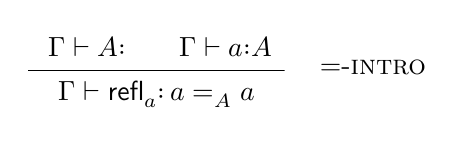
\begin{tikzpicture}[
    edge from parent path={
        (\tikzparentnode\tikzparentanchor)
        +(0pt,.5\tikzleveldistance)
        -- (0pt,-.5\tikzleveldistance -| \tikzchildnode\tikzchildanchor)
        -- +(0.75cm,0pt)
        -- +(-0.75cm,0pt)
    },
    grow'=up,
    level distance=4ex,
    level/.style={sibling distance=5em/#1}]
  \draw (2.75cm,.35cm) node {=-\textsc{intro}};
  \node (Concl) {\(\Gamma\vdash \textsf{refl}_a{:}\,a=_Aa\)}
    child { node (Major) {\(\Gamma\vdash A{:}\Univ\)} }
    child { node (Minor) {\(\Gamma\vdash a{:}A\)} } ;
\end{tikzpicture}

(Note that this is called the =-\textsc{intro} rule rather than
the \(\reflA\)-\textsc{intro} rule.)

\medskip

This means that we can always infer \(\reflAa{:}\,\reflAaa\) from just
\(a{:}A\); but it says nothing about any other proof of \(\reflAaa\),
nor about proof of \(\reflAxy\) for any other \(x,y{:}A\).  So even if
we have \(\reflAa\prec p\) for all \(\preflAxy\), we cannot invoke WFI,
since there is no constructive path from the former to the latter.

There is another problem with the informal explanation offered by the
HoTT book: it relies on a notion of induction as explanatory.  This
violates the general principle that types are explained by their
inference rules.  ``Path induction'' is explained by the ind-intro
(aka =-elim) rule, which has nothing to do with any antecedent notion
of induction.  It just lays down what it means to be an equality
proof.  We can call this induction, but then we're just labelling an
elimination rule -- misleadingly, since the elimination rule does not
involve and is not justified by any concept of induction.

On the other hand, one could argue that the formal rule captures some
intuitive notion of induction, just as the \&-intro rule captures our
informal notion of conjunction.  But the problem with that is, as
explained above, we do not seem to have an intuitive notion of
induction that corresponds to the =-elim rule.  On the other hand, we
do have intuitions about equality, but they do not depend on
intuitions about induction; they seem to depend mostly on practices of
exchange.

What we do with equalities seems to be fundamentally different from
what we do with inductive stuff.  Induction takes us from the
particular to the general; equality seems to be already general.  We
don't need to prove that one pebble is as good as any other for
tallying; it's built-in to the notion of tallying.  No induction is
needed; it doesn't make sense to try to ``test'' new pebbles to see if
they really work, or to prove that they do.  Using induction to
justify our ways with equality makes no sense.

\bigskip

\noindent
A possible way out is to reinterpret reflexivity as something that
follows from equality generally.  Then we can define a different
introduction rule for \(\reflA\).

\medskip

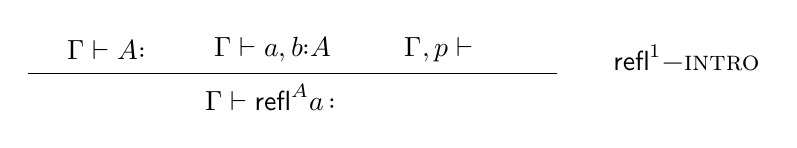
\begin{tikzpicture}[
    edge from parent path={
        (\tikzparentnode\tikzparentanchor)
        +(0pt,.5\tikzleveldistance)
        -- (0pt,-.5\tikzleveldistance -| \tikzchildnode\tikzchildanchor)
        -- +(1.5cm,0pt)
        -- +(-1cm,0pt)
    },
    grow'=up,
    level distance=4ex,
    level/.style={sibling distance=6em/#1}]
  \draw (5.25cm,.5cm) node {\(\textsf{refl}^1-\)\textsc{intro}};
  \node (Concl) {\(\Gamma\vdash \textsf{refl}^Aa\,{:}\,\reflAaa\)}
    child { node (Major) {\(\Gamma\vdash A{:}\Univ\)} }
    child { node (Minor) {\(\Gamma\vdash a,b{:}A\)} }
    child { node (Minor) {\(\Gamma,p\vdash \reflAab\)} } ;
\end{tikzpicture}

\medskip

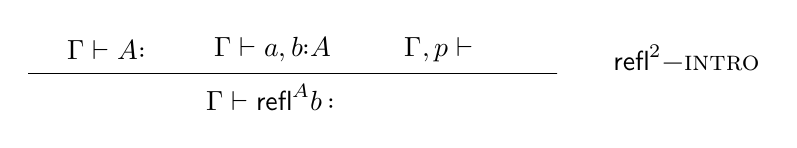
\begin{tikzpicture}[
    edge from parent path={
        (\tikzparentnode\tikzparentanchor)
        +(0pt,.5\tikzleveldistance)
        -- (0pt,-.5\tikzleveldistance -| \tikzchildnode\tikzchildanchor)
        -- +(1.5cm,0pt)
        -- +(-1cm,0pt)
    },
    grow'=up,
    level distance=4ex,
    level/.style={sibling distance=6em/#1}]
  \draw (5.25cm,.5cm) node {\(\textsf{refl}^2-\)\textsc{intro}};
  \node (Concl) {\(\Gamma\vdash \textsf{refl}^Ab\,{:}\,\reflAbb\)}
    child { node (Major) {\(\Gamma\vdash A{:}\Univ\)} }
    child { node (Minor) {\(\Gamma\vdash a,b{:}A\)} }
    child { node (Minor) {\(\Gamma,p\vdash \reflAab\)} } ;
\end{tikzpicture}

\medskip

The idea is that, instead of inferring \textsf{refl} directly from
\(a{:}A\), we can infer it from \emph{any} proof of \(\reflAab\).
This corresponds more closely to treating reflexivity as a binary
relation, rather than a unary predicate.  Reflexivity itself does not
\emph{introduce} equality, as the HoTT definition suggests; after all,
we can specify equality types without also introducing their proofs.

Rather, reflexivity is just the canonical form of proof of reflexivity
types, not of equality types generally.

This suggests another revision to the HoTT definition, this one a refinement:

\medskip

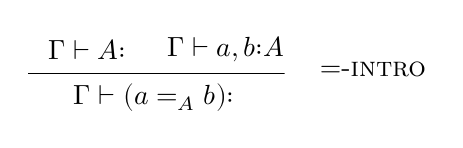
\begin{tikzpicture}[
    edge from parent path={
        (\tikzparentnode\tikzparentanchor)
        +(0pt,.5\tikzleveldistance)
        -- (0pt,-.5\tikzleveldistance -| \tikzchildnode\tikzchildanchor)
        -- +(0.75cm,0pt)
        -- +(-0.75cm,0pt)
    },
    grow'=up,
    level distance=4ex,
    level/.style={sibling distance=5em/#1}]
  \draw (2.75cm,.35cm) node {=-\textsc{intro}};
  \node (Concl) {\(\Gamma\vdash (a=_Ab){:}\,\Univ\)}
    child { node (Major) {\(\Gamma\vdash A{:}\Univ\)} }
    child { node (Minor) {\(\Gamma\vdash a,b{:}A\)} } ;
\end{tikzpicture}

\noindent which just says that given \(a,b{:}A\) we can form the
\emph{type} \(\reflAab\), independently of whether we can find a proof
of that type.  The introduction rules \(\refl{1}\) and \(\refl{2}\)
then just say that, given any proof \(p\) of \(\reln{A}{a}{b}\), we
can introduce the canonical proofs \(\refl{A}a{:}\reln{A}{a}{a}\) and
\(\refl{A}b{:}\reln{A}{b}{b}\).

\medskip

What would this mean for constructive WFI?  The core idea of WFI for
proofs on equalities is that to prove something for any equality proof
for any pair (of type \(A\)), it suffices to prove it for the
\(\refl{A}\) proof for reflexivity pairs; the justification is based
on well-founded structure.

With our revisions, any equality proof can be reduced to \(\refl{A}\),
which is more in line with the notion of canonical form as normal
form.  The intro rules do not mean that other proofs are constructed
inductively from the canonical proofs; but as they are indeed
introduction rules they set the meaning of \(\refl{A}\).  Instead of
proof by induction, we prove by normalization -- which in turn is a
kind of induction.  Normalization has well-founded structure; it
always bottoms out at canonical forms.

So it still suffices to prove the base case \(\refl{A}\).  Not
directly because of inductive construction, nor because of (classical)
well-founded structure, but because of an (axiomatic) principle of
normalization.  (?)

\begin{remark}
  In other words, if our intro rules allow us to infer canonical form
  from non-canonical form -- by fiat or axiom, as it were -- this is
  just as good as having an inductive constructor that builds other
  canonical forms from the base case.  For example, for \(\Nat\) we
  use \(S\) to build from \(Z\); but for =, we reverse this, saying in
  effect that non-canonical forms can be ``deconstructed'' and the
  canonical form pulled out.  We might be able to think of our
  \(\refl{A}\) intro rules as implicit elimination rules or
  co-constructors: they say that for any proof of equality we can
  extract the base case that must have been used to construct the
  proof, even if we do not have an explicit \(S\)-like constructor
  showing exactly how the proof was built up from the base case.
\end{remark}

\begin{remark}
  Or, there are two ways for WFI to work constructively, one based on
  inductive construction, and one based on inductive co-construction,
  so to speak.  The former method establishes a well-founded relation
  by construction; the latter by co-construction.  In the former case,
  you can always construct the ``next'' element; in the latter, you
  can always co-construct the base element.  Is this co-induction?  So
  equality proofs are codata?
\end{remark}

\medskip

Consider what the idea would look like for \(\Nat\):

\medskip

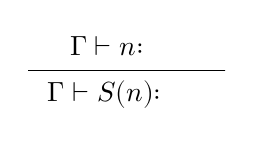
\begin{tikzpicture}[
    edge from parent path={
      (\tikzparentnode\tikzparentanchor)
      +(0pt,.5\tikzleveldistance)
      -- (0pt,-.5\tikzleveldistance -| \tikzchildnode\tikzchildanchor)
      -- +(1.5cm,0pt)
      -- +(-1cm,0pt)
    },
    grow'=up,
    level distance=4ex,
    level/.style={sibling distance=6em/#1}]
  %% \draw (5.25cm,.5cm) node {\(0{:}\,\Nat} ;
  \node (Concl) {\(\Gamma\vdash S(n){:}\,\Nat\)}
  child { node (Major) {\(\Gamma\vdash n{:}\Nat\)} } ;
\end{tikzpicture}
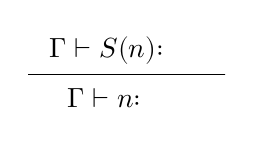
\begin{tikzpicture}[
    edge from parent path={
      (\tikzparentnode\tikzparentanchor)
      +(0pt,.5\tikzleveldistance)
      -- (0pt,-.5\tikzleveldistance -| \tikzchildnode\tikzchildanchor)
      -- +(1.5cm,0pt)
      -- +(-1cm,0pt)
    },
    grow'=up,
    level distance=4ex,
    level/.style={sibling distance=6em/#1}]
  %% \draw (5.25cm,.5cm) node {\(0{:}\,\Nat} ;
  \node (Concl) {\(\Gamma\vdash n{:}\,\Nat\)}
  child { node (Major) {\(\Gamma\vdash S(n){:}\Nat\)} } ;
\end{tikzpicture}
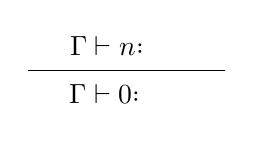
\begin{tikzpicture}[
    edge from parent path={
      (\tikzparentnode\tikzparentanchor)
      +(0pt,.5\tikzleveldistance)
      -- (0pt,-.5\tikzleveldistance -| \tikzchildnode\tikzchildanchor)
      -- +(1.5cm,0pt)
      -- +(-1cm,0pt)
    },
    grow'=up,
    level distance=4ex,
    level/.style={sibling distance=6em/#1}]
  %% \draw (5.25cm,.5cm) node {\(0{:}\,\Nat} ;
  \node (Concl) {\(\Gamma\vdash 0{:}\,\Nat\)}
  child { node (Major) {\(\Gamma\vdash n{:}\Nat\)} } ;
\end{tikzpicture}

\medskip

\noindent Here the rule on the left just expresses the definition of
\(S\) for \(\Nat\).  The rule on the right expresses a kind of
elimination rule - we know any \(n{:}\Nat\) must have the form
\(S(S(...S(0)))\), so it expresses the idea that all of the \(S\)s
could be eliminated.  We could prove this, since any \(n{:}\,\Nat\) is
inductively constructed.  But were that not the case, we could simply
stipulate it as part of the definition of what it is to be of type
\(\Nat\).  And that's what we do for equality types and \(\refl{A}\).

\subsection{Coinduction}



\subsection{Reflexivity Induction}

For any reflexivity type \(\reflAa\) we may have infinitely many proofs
\(\preflAa\).  The HoTT book singles out just one such proof per type
and designates it as the canonical constructor for the type:

\begin{align}
  &\textsf{refl}{:}\,\reflfam &  \textsf{HoTT p. 48} \\
  \intertext{(which should be:)}
  &\textsf{refl}{:}\,\reflfamU \\
  \intertext{giving}
  &\reflA(x):\,(x\circ_A x)
\end{align}

Which makes \(\reflA\) a family of ``provers'' of reflexivity types:
give it an \(x\) and you get a (canonical) proof of \(\reflTAx\).

Since we may have non-canonical proofs \(x{:}\reflAa\), we are
confronted with the task of showing that if a predicate on proofs of
\(\reflAa\) can be satisfied by one such proof it can be satisfied by
any such proof.  This is what path induction is for (although it
extends beyond reflexivity types to all \(x\circ_Ay\) types).

A predicate on proofs of \(\reflAa\) looks like this in the HoTT book:

\begin{align}
  & \Cxyp & \textsf{HoTT p. 49} \\
  \intertext{giving}
  & C(x,x,\reflx){:}\,\Univ
\end{align}

\noindent We rewrite this as:

\begin{align}
  & \SXYPT \\
  \intertext{giving:}
  & \SXX \\
  & \SXXP
  \intertext{and we set}
  & S^{x\circ_Ax}(p) :\equiv \reflTAx
\end{align}

We use \(\circ\) instead of \(=\) for generality, and we use
\(S^{\circ_A}\) intead of \(C\) in order to highlight that fact that
we treat it as a (not ``the''!) successor type family drawn from
\(\circ_A\) types, so \(\SXXP\) is \emph{a} successor type at \(p\)
from type \(\reflTAx\) -- which in turn we treat as \emph{a} successor
type at \(x\) for \(x\) from \(A\).

Note that for any \(\preflTx\) we have \(p{:}\,S^{x\circ_Ax}(p)\):
every proof of \(\reflTAx\) is proof of its own successor type.  Or: if
p proves a successor type at x for x, the it also proves its own
successor drawn from that successor type at x for x.  Reflexivity all the way
up!


\medskip

Now the HoTT book bases path induction on \(\reflAx\), which is an
element of \(\reflTAx\); informally, the path induction principle for
reflexive types can be expressed by saying that a proof of a predicate
on \(\reflAx{:}\,\reflTAx\) suffices as proof on all \(\preflTx\).

\bigskip

The approach adopted here is a little different.  First, we don't
single out a canonical constructor.  Intuitively, the idea is that
since all proofs of \(\reflTAx\) are ``equivalent'', it should be
enough to prove the predication for any such proof; there is no call
to single out a canonical one.

\begin{remark}
I suspect that introducing a canonical element for reflexivity
types was motivated by the example of the inductive definition of
\(\Nat\), which has two canonical constructors.  And it is the
inductive structure of those constructors that makes proof by
mathematical induction work.  But the elements/proofs of equality
types are not constructed in this way; there is no sequential
structure to them.  But this suggests that we do not really need a
canonical constructor.
\end{remark}

\begin{remark}
  Note that mathematical induction is a little ambiguous.  Once you've
  proven for base case and inductive hypothesis, you drawn the
  conclusion to ``all n''.  But the justification for this inference
  is the intuition that ``all n'' are in fact constructed using the
  canonical constructors, so ``all n'' really means ``all canonical
  n''.  There is no good intuition (for me, at least) leading from
  ``all canonical n'' to ``all n including non-canonical/exotic n''.
  But that reading is essential to HoTT induction, and I suspect it is
  the real innovation.
\end{remark}

\bigskip

The basic idea is that we replace the notion of a canonical element
\(\reflAx\) with the notion of a canonical successor function.  This
gives us a genuine kind of induction: starting with any \(\preflTx\)
we get a ``next'' object, namely the successor type at \(p\).  There
are infinitely many successor families, and thus successor types at
\(p\); the intuition behind ``reflexivity induction'' is that proving
the canonical successor type for some \(\preflTx\) suffices as proof
for all such \(p\), for all successor types.  In other words, if you
can prove the canonical successor proposition \emph{at p} for some
\(\preflTx\), you can prove any successor proposition \emph{at p} for
any such \(p\).

So what our approach boils down to is moving from elements/proofs of
reflexivities to their successor types/propositions, which are what we
want to prove.  This gives us an inductive structure, analogous to the
structure of \(\Nat\), that the HoTT approach, based on canonical
elements, lacks.  Well, it's not so much that it goes missing as that
it goes unremarked.  What I sketch here is implicit in the HoTT book.

In other words, it is not the case that all elements of \(\reflTAx\)
are inductively constructed from canonical constructors, but it is the
case that the successor type of every such element is inductively
constructed by a successor function.  In contrast to e.g. \(\Nat\),
whose structure can be thought of as ``vertical'', the inductive
structure of reflexivity proofs combines ``horizontal'' and
``vertical'' aspects.  The successor types are all at the same level,
one level ``up''from the elements to which they are successors;
neither can be ordered.  But nonetheless each pair of element and
successor type has inductive structure, from n to n+1.

A critical point is that we do not need a canonical element to do
this; we need not define \emph{any} constructors for reflexivity
types.

Once this structure is clear it also becomes clear that the inductive
principle required to make this work is clearly not like the inductive
principles involved in the three basic kinds of induction.  The
proposal here is that it is this induction principle that is
distinctive, rather than the Id/= type family specified in the HoTT
book.

The implicit reasoning: we prove that if something is true for
arbitrary \(n\) (i.e. for any \(\preflTx\)) then it is true for
\(n+1\) (i.e. \(p{:}S^{x\circ_Ax}(p)\)).  We then infer that it is
true, not for all \(n\) (there are only two levels, \(n\) and \(n+1\),
and we've already shown the equivalent of \(P(n)\to P(n+1)\) for
arbitrary n) but for all successor types (propositions) in the family
\(\prod\limits_{(x,y:A)}\prod\limits_{p{:}(x\circ_Ay)}{:}\,\Univ\).

In other words, mathematical induction goes from \(P(n)\to P(n+1)\)
for arbitary n to \(P(n)\) for all n; we go from \(P(n)\to P(n+1)\)
for arbitary n to \(Q(n)\) for all \(Q, n\).

Hmm, that can't be right.  Some successor props may not be
satisfiable.  We have to do the inductive proof for each successor
type.

Since we don't use a canonical element, there is no move from ``true
for canonical'' to ``true for everything''.  We don't even need to
move to ``true for everything'', since we prove the inductive step for
arbitrary n?  No, proof for arbitrary n is not same as proof for all;
you have to make the inductive inference to get from the former to the
latter.  So we need it too.

What's our base case?  Refl?  Hmm, that would suggest that path
induction is wrong, its missing the inductive step that we have
articulated.

Writers on HoTT (Ladyman?) say that the inductive step goes missing in
path induction; we go straight from base case to generalization.  That
makes no sense to me.

The formal definition of HoTT weasels out of this be defining ind= as
a primitive elimination rule.  But that sticks in my craw too; it just
seems wrong to encode induction as an inference rule the way HoTT does
it.  It should be structured just like the traditional inductions:
base case, then inductive hypothesis, then generalization:

\begin{itemize}
\item Base case:  \(\reflAx{:}\,\reflTAx\to \reflAx{:}\,S^{x\circ_Ax}(\reflAx)\)
\item Inductive hypothesis:  \(\preflTx\to p{:}\,R^{x\circ_Ax}(p)\) for arbitrary \(p\)
\item Generalization:  \(\preflTx\to p{:}\,S^{x\circ_Ax}(p)\) for arbitrary \(p\)
  %% \(S^{x\circ_Ax}(p)\) for all \(\preflTx\) and for all \(S\)
\end{itemize}

Critical move: defining \(S^{x\circ_Ax}(p) :\equiv (x\circ_Ax)\).  Is
that kosher for all successors?  No, the successor type at p can be
anything.  We need canonical reflexive successor:  \(\RXXP\).

The problem is we have two variables: proofs of x=x, and successor
types at those proofs.  To generalize over the latter we must use
conditionals.

Goal is to show that for arbitrary successor S, if S(p) for some
p:x=x, then S(p) for all p:x=x.

\begin{itemize}
\item Base case:  \(\preflTx\to p{:}\,R^{x\circ_Ax}(p)\) for arbitrary \(p\)
\item Inductive hypothesis: function from S(p) to ?? for some p?
\item Generalization: function from S(p) to ?? for all p?
  %% \(S^{x\circ_Ax}(p)\) for all \(\preflTx\) and for all \(S\)
\end{itemize}


\subsection{Recursion}

%% https://en.wikipedia.org/wiki/Course-of-values_recursion

\section{Construction and Co-construction}

The standard presentation of intuisionistic/constructive mathematics
says, in so many words, that you must be able to construct stuff.
This means that if we think we have something but no means of
constructing it, we're in trouble.  Case in point: equality proofs in
HoTT.

But the concepts of coinduction and bisimilarity suggest a more
refined notion.  Construction builds up; co-construction builds down.
If you can start at the base case and build your object using
canonical constructors, you have a construction.  If you start at your
object and ``build'' - that is, co-construct - a base case, then you
have a co-construction.

In other words, it is sufficient for constructivity to be able to get
(co-) constructively from your object to a base case.  If you can do
that, then you are working (co-)constructively, even if you have no
method of constructing your object from the base case.

This corresponds to the idea of ``hidden'' stuff addressed by
bisimilarity.  In this case, the constructive form of the object is
hidden; but since we can co-construct downwards we can infer that the
object is indeed a construction even though we cannot ``see'' the
construction.

\begin{remark}
  What I'm calling co-construction seems to be called ``observation''
  by some authors.  Suggesting that we might think of elimination
  rules as observational rules.  This makes sense; if we have
  arbitrary \(x{:}\,A\), the elim rules tell us how it behaves, not
  how it is constructed.
\end{remark}

\subsection{State Space v. Construction Space}

Can we think of vars like \(x{:}\,A\) in terms of a (hidden) state
space, by analogy with bisimulation?  We don't know how \(x\) was
constructed, but we can ``observe'' it by using eliminators, etc.
Instead of hidden state, hidden construction (structure).

\section{Grounding Equality: Pragmatics of Fair Exchange}

The task is to capture our ordinary intuitions about equality, just
like Turing captured our intuitions about effective procedures.
Similar: logical consequence.  So far nobody has managed to do for
logical consequence what Turing did for effective procedure:provide
something formal that captures our ordinary intuitions.  Ditto for
equality.  (TODO: quotes about problems with equality)

Paradigm: fiat currency.  Each dollar bill is "equal" to each other.
But each is also different, as a physical particular.  What makes them
equal is exchange value, which is socially instituted.  So equality is
a social institution.

Equality as exchange value depends on token recognition, so the
ability to recognize that a particular is a token of a type - this
thing is a \$1 bill - is more primitive than equality, but also enables
equality.  This dependency can be made explicit by writing a =\$ b
instead of a = b, meaning that a and b are equal under the
\$-denominated currency regime - that is, under a particular
perspective.  So equality is always perspectival, which translates
into equality-as-type in HoTT.

Proof of equality: type theories like HoTT need a "proof" for each
equality type; usually this is defined as refl.  But the formal
structure of such definitions in a type theory does not capture our
ordinary intuitions about equality.  We can replace the (arbitrary)
symbols "=" and "refl" with any others without changing the meaning;
in particular we could use "Unit" and "*", respectively, giving "*a :
Unit a a instead of "refl(a): a = a" (leaving type A implicit).  So
the formal definitions have no conceptual content except what is
instituted by the introduction and elimination rules.  We cannot rely
on antecedent notions of equality and reflexivity; the latter in any
case is a specifically mathematical concept, relatively remote from
our ordinary intuitions, and so cannot be counted as primitive.

What counts as "proof" for our ordinary notion of equality, the one
involving exchange value?  We cannot count on merely "knowing that a
and b are the same" (HoTT p. 47 "The basic way to construct an element
of a = b is to know that a and b are the same.")  That approach runs
straight into Hume's problem.  Recall that Hume pointed out that we
cannot observe causality.  We can observe event a, and event b, and we
can observe that b invariably follows a; but we cannot observe a
causal connection between the two, and so we have no iron-clad
guaranteed that b will always follow a in the future; we cannot "know"
that a causes b.  Similarly, we can observe that a is a \$1 bill, and
that b is a \$1 bill, but we cannot observe a relation of equality
between them; we cannot "know" by observation that they are equal.  Of
course we can know that they are both \$1 bills - tokens of the same
type - but that does not count as knowing that they are equal.  (Or
does it?  We might also say that we can know that they are equally
tokens of the same type but that gives us no means of demonstrating
that knowledge - there is no "type of knowing that two things are
equal".  Then again, knowing that a and b are tokens of a type is
knowledge of a "vertical" relation between token and type; the
"horizontal" relation of equality between such tokens is a different
thing.) As mentioned above, equality is a social institution, not an
observable, "objective" property.  The only way to demonstrate
("prove") that a and b are equal is to actually exchange them and have
both parties to the exchange come away thinking the exchange was fair.
So we could simply define "refl" to mean "act of exchange"; but that
doesn't seem very mathematical, since actions are dynamic and
mathematical objects are not.  What we need is an actual physical
token that counts as proof of the equality in the same way that a \$1
bill (or coin) counts as "proof" of \$1.

Demonstration as proof: note that the notion of proof in HoTT and
similar extends our ordinary notion of proof.  We don't ordinarily go
around saying that, e.g. 2 proves Nat, but in type theory that is
exactly what "2:Nat" means (or at least it is one accepted gloss of
the notation.)  But if we change "proves" to "demonstrates" we have
something a little less odd: SS0 (=2) demonstrates Nat just because on
inspection we can see that it is composed solely of the constructors
that define Nat, assembled according to the rules of the type theory;
it "shows" Nat in action, so to speak.  Note the close connection
between compositionality and demonstration (proof); it's not
accidental.  Similarly it makes sense to say that a \$1 bill or coins
demonstrates the concept of \$1, and that fair exchange of dollar bills
demonstrates their equality.

So what physical token would count as demonstrating the equality of
two \$1 bills?  Here again we rely on a social institution: a contract.
Instead of actually exchanging dollar bills, the parties can agree to
such an exchange, and certify their agreement by writing and signing a
contract that obliges them to make the actual exchange some time in
the future.  The contract then serves as a physical demonstration of
the equality of the goods to be exchanged.

Notice that this does not really count as "proving" anything in the
traditional sense of exhibiting justification.  Indeed, in light of
the fact that equality is a social institution, it doesn't even make
sense to try to prove that one \$1 bill is equal to another.  That
would make it sound like there is some kind of equality property or
relation that we can discover and exhibit, or that there is some fact
of the matter that we can expose.  But there is no fact of the matter,
nor is there any "objective" equality relation to be "proved":
equality is social and perpectival.  Things are equal only because we
agree to treat them as equal, and this applies as much to mathematics
as to medium sized dry goods.  To social instutions of mathematics may
be complex, but they remain social institutions.

To put it another way: proof of equality /institutes/ equality; fair
exchange of a pair of 1\$ bills is just what makes them equal.

(But: isn't that always the case?  Proof of P institutes P?  Not
classically; there, propositions and proofs are ontologically
distinct.  Classical proofs justify (assertion of) propositions;
intuitionistic/inferential proofs institute propositions.  A
proposition demonstrated cannot be ontologically severed from its
demonstration.)

So we can view "refl" as a kind of contractual certification of
equality.  On this view, it has nothing to do conceptually with the
notion of reflexivity - it does not mean that a thing stands in a
binary relation of reflexivity to itself; it means that two distinct
things have equal exchange value.

The critical observation here is that the "reflexive" formula "a = a"
contains not one but two distinct 'a' tokens.  They are not "the
same", any more than two distinct \$1 bills are the same.  But they do
have the same exchange value, which is the same exchange value that
all such 'a' tokens have.  So we can take "a = a" as an inference
rule, one that licenses exchange of 'a' tokens.  Then "refl(a) : a = a"
reifies that license, so to speak, in the form of token "refl" whose
role is to certify that such exchanges are fair.

Key point being that this avoids the notion of reflexivity as a binary
relation of a thing to itself.  We could make this more perspicuous by
replacing "refl" with something like "exch", or even some variation on
the "=" symbol, e.g.  "a=a! : a = a", meaning "a=a!" certifies that
all 'a' tokens have equal exchange value.

Another critical point: we derived "exchange value" from ordinary
practices, but we can also derive it solely from type theory
primitives by means of a notion of token repeatables, or maybe even
token reflexivity.  Token repeatables are always interchangeable.
Each token, qua symbol, "gives rise" to the type of its token
repeatables.  E.g. we have 3:Nat; but we also have the type of such
3-tokens (token repeatables), so every "occurence" of the symbol '3'
is a token of that type.  To make this explicit we probably need a new
type former that turns tokens into token-repeatable types.  Then we
can say e.g. 3:T(3), where T(3) names the type of all 3-tokens.  By
definition, every token of a T-type is interchangeable with every
other token of that type.

Normally we do not actually exchange such tokens, instead we just
write down fresh copies and count that as using the same token.  But
we could physically exchange them; we could cut the tokens out of our
piece of paper and shuffle them around.  So for a = a, we could
actually cut out those 'a' tokens and paste either of them in place
wherever we need an a-token in our proof.

No constants and no vars - the distinction presupposes denotational
semantics.  But in type theory we only have tokens and types.  When we
write \(x:A\) what we mean is that the inference from the particular
token \(x\) (which is token-repeatable) to type \(A\) is
\emph{assumed}, not that \(x\) is a variable of type \(A\) waiting for
assignment.

E.g. x:Nat, x = 1+1.  The latter does not mean ``assign the value of
1+1 to symbol x''; nor does it mean something like ``(it is true that)
the values of x and 1+1 are equal''.  It just means that we are
licensed to exchange x tokens and 2 tokens.



**************** old:


Goal is to explain type theory

    * in terms of the ordinary intuitions of lived experience

    * without relying on representational vocabulary like "refers", "denotes", etc.

    * without metaphysics or psychologism

The approach draws on Brandom:

    * normative pragmatics

    * inferential semantics

    * logical expressivism

Surprising results:

    *  the Unit type is incoherent

    * identity types (aka token-repeatable types) are primitive, all
       others derivative (in the order of explanation); this is
       because tokens are always repeatable, which gives rise to a
       type (token-repeatable type)

    * constructors are not functions; the former are primitive, the
       latter derivative

The starting point is the type-token distinction.  We show how this
relation can be explained in terms of practical norms instituting the
treatment of particulars as tokens of a type.

What is a type?  A type is an institution.  What is a token?  A token
is a particular in a functional role.


Token-particulars and perspectivism.  The only way a particular can
function as (play the role of) a token of a type is for us to treat it
as such.  We move from particular to token-particular - that is, from
particular to particular-as-token.  This is an inferential move, from
to particular to category.  It's inferential because categories
(concepts) are inferentialy articulated.  What Sellars called a
language-entry move.  But this move does not require language.  Or
rather categorization does not, though conceptualization does.  Even
primitive life forms categorize; in fact inanimate things categorize
(Brandom's example of a chunk of iron, rusting.)  But since we're
talking about human practices, it is proper to view the move from
particular to token-particular as an inferential move; let's call it a
token inferencing.

Token inferencing is a two-fold move: from particular to token of
type, i.e. inference to both type and functional role. (?)


A good "intuition pump" for illustrating the pragmatic basis of type
theory is the practice of tallying.  Before we can even begin to tally
- e.g. by dropping pebbles into a pouch, notching a stick, etc. - we
must have mastered the inferential practices involved in recognizing
particulars as tokens of a type.  We must have the practical ability
to treat distinct pebbles as indistinguishable tokens of a type - call
it Counter.  And this is a matter of practical norms - we treat
countings using pebbles as correct or incorrect, and that's about as
far as explanation can go.  It would be fruitless to try to explain
why or how we manage to recognize that a particular object is a
pebble; the best we can say is that treating it as a pebble just like
all the others is the correct thing to do.

So token inferencing is a primitive practice that precedes more
sophisticated token/type practices like tallying; the latter depends
on the former.  Neither depends on language; both are essentially
normative, practical skills.

The critical point here is that (the practice of) this sort of
inferential skill (token inferencing) is what institutes concepts.
Creatures can treat particular pebbles as tokens of a (nameless) type
even if they have no language; in fact, they do not even need an
antecendently available concept of type (or of "concept").  But once
they have instituted such normative practices they can say what they
otherwise can only do by expanding their vocabulary.  They can invent
words like ``that'' and ``pebble'', and go around point at things and
declaring "that pebble"!  Doing so makes explicit the normative
practice of treating things as pebbles; it makes the language-entrance
move explicit as a correct move.  The village idiot can go around
pointing at cows and exlaiming ``that pebble!'', but the other
villagers will treat him as linguistically incompetent.  ``That
pebble!'' as a kind of rule, which can be applied correctly or
incorrectly.

This is just what the standard type-theoretic notation "a : A" does.
Most expositions of type theory gloss this as "a has type A", or "a is
proof/witness/inhabitant of A", etc.  The proposal here is that we
should read this expression as exactly analogous to a propositional
implication like A -> B.  But only analogous; A -> B is a schema
licensing inference from proposition to proposition, whereas we treat
"a : A" as a schema licensing inference from particular to
token-particular.  We gloss it "from a infer A" or "from particular a
infer type A", or "infer that particular a is a token-particular of
type A".  It's also stipulative, not empirical; remember 'a' is a
token, not a symbol.

Note that token inferencing is perspectival; particulars only come to
play the role of tokens (i.e. are correctly treated as tokens) within
the context of particular purposes or "language games".  So it might
be better to gloss "a : A" as "treat particular a as a token of type
A, for the purpose at hand."  (Remembering that inferencing is
something we do that involves /treating/ things in correct ways, so to
treat a as a token of type A is to make a practical inference from
particular to token-particular.)

[Constants: 3:Nat is a rule licensing use of 3-tokens according to the
  rules of Nat.]


[FIXME: Now there is a (very) subtle but critical point here that is
  obscured by our very use of language.  We naturally tend to
  abstraction; most of us will treat the "a" in "a : A" not as a
  particular but as either a constant symbol that denotes a particular
  or a variable symbol that ranges over a collection of particulars,
  or maybe even an "unknown".  In any case, before it is any of that
  it is indeed a particular - a particular bit of ink on paper, or
  illumination on a screen.  And remember we have ruled out any appeal
  to denotation, so we cannot take the tokens in our expressions as
  refering to anything.]

But if "a : A" is an inference license (or: an inference that
institutes a license, i.e. a rule), don't we need to already know what
"a" is to proceed with the inference?  Only under denotational
semantics.  [Cmp. Platonic anamnesis] It can't mean "treat any old
thing as an A-token".  But if it just means "an A-token is an A-token"
then it does not involve inference.  The point is that a:A does not
express some relation or between or ``true'' fact about a and A that
we have discovered.  It makes no sense to say ``a:A'' is true, because
it is not a proposition, it is an inference (rule) that does not
depend no denotation .

The issue comes out more clearly if we go back to tallying practices
using pebbles.  It should be obvious that the pebbles involved in the
practice of tallying do not denote anything; in fact they are not even
symbols.  They are particulars; distinct entities located in space and
time.  Particulars are distinct by definition; to say that one two
particulars are "identical" is nonsensical, and to say that one
particular is identical to itself is vacous (Wittgenstein said
something like this, I believe.)  To move from particular to
token-particular means to ignore the particularities (the identity) of
the particular.  And it is by doing this that the notion of type
emerges (is instituted).  The Platonist might say that a particular is
a token of type A because it somehow (mysteriously) "participates" in
ideal A; the Aristotelean, that we somehow (mysteriously) derive the
abstract A from particulars.  The pragmatic perpective eliminates the
mystery: it is only by virtue of our treating particulars as A-tokens
that the type A and the role of A-token are instituted.

This has two subtle consequences that are not generally noticed in
type theories.  One is that the notion of a Unit type, with only a
single "element", is conceptually incoherent.  A type with only one
element would not be a generalization; the notion of type essentially
involves a plurality of tokens.  But can we not just stipulate that
type Unit has only one token?  We can try, but it won't work, since
that token is itself "repeatable".  In HoTT terms, if we have * :
Unit, we can create as many * tokens as we please.  The critical point
is just that these iterated tokenings are precisely *not* the same, or
identical, or equal: they are particulars.  We /treat/ them as the
same; but just think about it: that means we treat them as "identical
instances" of the one Tau type T(*).  And this illustrates the second
subtlety: it means that we are treating our one token itself as a
(proxy for a) type.  In fact every token of every type gives rise to
this sort of type, which we can call something like a token-repeatable
type.  People familiar with HoTT may recognize this as none other than
the Identity or Equality type of HoTT.

In other words, token-particulars have an inherently dual character.
On the one hand they are particulars; on the other hand, they are
/treated/ as indistinguishable tokens.

For example, we have 3 : Nat, glossed as "3 has type Nat".  But 3 also
is a type, namely the type of all 3-tokens.

Here's a more vivid example.  Using the standard inductive definition
of Nat, with Z and S as base case and successor, respectively:

    S S Z = S S Z

which says that 2 = 2.  The traditional way to explain this is in
denotational terms: the right and left hand sides of this equation
denote the same thing, which obviously must be the case since they
have the same form.

But the right and left sides of the equation are \emph{not} equal;
they are distinct particulars; they are not the same thing.  And since
we cannot appeal to denotation, we cannot say that they are the same
by virtue of denoting the same ``value''.  One way to explain the
meaning of this equation is to treat the two subexpressions as
distinct tokens of type T(2), which yields the following reading:

  "S S Z = S S Z" means that each "S S Z" token has type T(S S Z).

[BUT: what justifies this?  Only our exchange practices.  Go back to
pebbles, where each token is clearly a distinct physical particular,
and emphasize that every S and Z we write down is just as particular.
It is only our practice of treating such particulars (and their
accumulations) as interchangeable that institutes the idea of
equality.]

This is why it makes sense to say that a and b can be equal in more
than one way.  It just means that they are token repeatables.  And it
is always possible to ``create'' a new token, e.g. strike a new tally
mark or pick up a new pebble.

[FIXME: so we have two ideas we need to disentangle.  Once is
token-inferencing, the other exchangeability.  Plus the idea of a constructor.]


[We can treat token repeatables as ``the same'' effortlessly, without
  explicit rules; but this is precisely what machines cannot do, and
  that is why we need equality types in formal languages.]

In other words, the pragmatic perspective, emphasizing normative
inferential practices and particulars, leads directly the HoTT notion
of equality types.  But it explains that concept, not in terms of
equality of identification of tokens, but in terms of inference from
particular to token-particular - that is, to token-repeatable type.

And ultimately this is grounded in norms governing exchange or trade.

Concrete illustration: counting to two using two particular pebbles
can be done in two ways.

Also, treat e.g. S S Z as exactly like dropping pebbles - the S tokens
are particulars; they are every bit as particular as particular real
pebbles.

So every Nat "element" is a token-repeatable type.  E.g. any
particular 3 token has both type 3 and type Nat.

Constructors: in tallying our pebbles are constructors.  They are not
functions.  Ditto for S and Z: SSZ does not denote a number as result
of a function, it just /is/ a token from which we can infer Nat:

    SSZ : Nat

That is, SSZ is a particular (containing three particulars) that we
treat as a 3-token, which we treat as a Nat-token.  For this to be
intelligible we have no need of a function concept.  This is obvious
in the case of Z, which is analogous to our empty pouch.

More precisely: SSZ functions as (has the role of) a Nat in our game,
and S and Z function as tokens in that game; we can use tokens to
construct other tokens (e.g. adding an S token to SZ); but tokens are
not functions.  They don't do anything, although they /have/ a
function: they can be used (by rule) to construct new tokens.

Calling a ctor a function that constructs values of a type is like
calling a brick a function that builds walls.

Actions as types and tokens: concrete act of dropping a pebble as
token of type Tally (or TallyAction).  Then equality becomes
equivalence of action.

Reflexivity: a=a as a type is just the token-repeatability type of a,
and every a has this type; refl just means that each token of this type
is a token of this type.  Its a relation of token to type rather than
token to itself.

Tau types: every token is (naturally?) associated with a type, the
type of its token-repeatables.  The tau operator is analogous to
Church's lambda operator: just as lambda turns an open formula into a
name of its associated function, the tau operator turns a
token-particular into the name of its associated token-repeatable
type.  For example, T(2) names the type of all 2 tokens.

Now every token of a tau type is substitutable for any other token of
the same type; that's just what token-repeatable means.  (Particulars
are not repeatable, but token-particulars, that is tokens, are.)

Recall that "a : A" means that the inference from a to A is good.  So
e.g. a : Tau(2) means that the inference from a to Tau(2) is good.
What a : Tau(2) does not mean is that a is itself a 2-token.  So an
expression like 1+1 : Tau(2) is intelligible; it just means that from
the token 1+1 we can infer Tau(2).  And it makes sense in practice,
because we can (by the rules of the system) convert "1+1" to "2", and
we have 2 : Tau(2) by definition.  And notice that it works just as
well the other way around: 2 : Tau(1+1).  To make the inference, we
just rewrite 2 to obtain a "1+1" token.

Equality is closely related to tau types.  "a = b" means that a and b
are substitutable.  But we interpret substitution as an inference: "a
= b" means that the inference from any expression involving a to the
same expression with b replacing a is a good one.  So the equality
operator "=" is best thought of as an inference op.  To make this more
conspicuous we'll write "==>" instead of "=".

Caveat: a ==> b does not mean "from a infer b"; it means rather
something like "from any expression containing a, e.g. SEXP[a], infer
SEXP[b/a]".

How to relate tau types and this inferential interpretation of
equality?  How should we interpret e.g. "1+1 = 2"?  And what would
count as a "proof" of it?

First, a substitution inference rule is a schema; that means that the
rule a ==> b is not about the particulars embedded in the rule.
Rather, it relies on the implicit tau types T(a) and T(b); the
explicit formulation should be a:T(a) ==> b:T(a).

[NB: problem with the HoTT definition that given a:A and b:A, form
type \(a =_A b\).  This allows us to form e.g. 2 = 3.]

But (in HoTT at least) "a = b" just another way of expressing the Id
type: Id(a,b) (We're omitting the type sym A.), whose canonical
element is refl(a).  And this looks suspiciously like Tau(a).

The problem with the HoTT book is that it does not explain this, it
just glosses it with the very improbably "[t]he basic way to construct
an element of a = b is to know that a and be are the same".  There are
two problems with this gloss.  One is that "the way to construct... is
to know" makes no sense; constructing and knowing are not the same
thing.  The second and more basic problem is that the text offers no
explanation of what it is to know that a and b are "the same".  The
whole discussion is circular.  Equality, identity, sameness, and
related terms come out as unexplained explainers.

By focussing on normative practices of treating particulars as tokens,
treating token exchanges as correct, etc., we can offer a genuine and
non-mysterious explanation of the vocabulary of equality.  Terms like
equals, identification, etc. come out as explicitation devices that
allow us to say explicitly what we can otherwise only do in practice:
treat particulars as tokens, and treat one token as substitutable for
another for a particular purpose.  By foregrounding inference,
equality naturally emerges as a rule of (substitution) inference, and
since rules institute types, exchange practices institute equality
types, which the terminology of equality makes explicit.

Under this perspective the equality or identity types come out as
primitives - that is, primitive inference rules.

What about tau types?  There doesn't seem to be anything like a tau
type in the HoTT book.  But a tau type really just is the HoTT Id type
under a different perspective.  But there are differences.  In HoTT,
equality types are expressed in terms of two tokens of a single type:
given a:A and b:A, form the type \(Id_A(a,b)\) (equivalently, (\(a =_A b\)))
with canonical witness refl(a).  As noted above this does not rule out
things like "2 = 3" with witness refl(2).  Also, HoTT does not really
address the distinctions we've made between particulars,
token-particulars, token-repeatables, etc.  (I suspect that is because
the authors have a tendency to continue to think in
representationalist terms, which is not surprising since its a very
natural tendency).

So a question is: can we recover HoTT's Id types with their refl
witness just from our tau types and substitution-inference rules?


Token indiscernability: to treat a particular as a token-particular
(that is, as a particular that "has" some type) is just to treat it as
indiscernable from other token-particulars of the same type (for the
purpose at hand).  But "indiscernability" is an arcane philosophical
concept.  The practical basis for it is the normative practice of
substitutability or exchangeability.  It is only because we treat
particulars as tokens, and further because we treat tokens of the same
type as interchangeable, that we can speak of indiscernability.  We
don't need the philosophical apparatus of properties, satisfaction,
etc. to make sense of this.

(Compare chess pieces: distinct as particulars, but treated as
indiscernable - it doesn't matter which rook you put on the right or
left, though which rook you move does matter.  But even then you move
right or left rook, not this or that particular.  It's the position on
the board that makes them discernable not their properties as
individuals.)

So substitutability and token inferencing (or "tokenization"?) seem to
be equally primitive.  You cannot go treat a particular as a
token-particular unless you can also treat particulars as
substitutable "under the type".  Alternatively: it is not possible to
play the game of tokens and types if you cannot also play the
substitution game.  And vice-versa.

In more formal terms: tau types are primitive.  They are an
explicitation of the norms of both tokenization and substition
practices.

Natural types v. fiat types: the counter or pebble types in our
examples count as natural types.  They are instituted by our practices
but do not involve explicit rules.  The types of type theories like
HoTT are fiat types: they are instituted by explicitly articulated
rules.  Nevertheless the meaning of those rules is to be
explained in terms of normative practices.

Types as institutions, literally.

refl as token of type Tau(a).  What would count as a physical token of
equality in our tallying game?  In HoTT terms: to prove something for
all T(a) tokens, it suffices to prove it for ... T(a) itself?  Or any
T(a) token?  With the concept of T(a) we loose the notion of canonical
constructor.  Unless we want to treat Tau itself as the canonical
ctor.

But: tokens are not physical, particulars are.  Tokens (and types) are
(functional) roles, rules in the game.  So even our pebbles are not,
strictly speaking, physical tokens.  So a better question to ask is:
what plays the role of an equality token (i.e. a "proof" of equality)?
Answer: tau types?  A tau type T(a) is just the role that particulars
may play, as a-tokens.

Primary v. secondary identity.  Particulars have identities; this is
primary identity.  Token-particulars play roles: this is secondary
identity.  Each red checker piece has an identity as a particular; no
two pieces are identical in this sense.  But qua game pieces, they
play "the same" role; they are all "identical" in this derived sense.
And what is identical is not the pieces themselves, but the role they
play, since there is only one such role: red game piece.  Not the
pieces but their roles are "the same".  Every token-particular has two
identities in this sense, one primary (or primitive) and the other
secondary (or derived).  Derived from both primary identity and the
rules of the game.  The rules of the game institute the derived
identity, but the play that role, a game piece must (antecedently)
have primary identity, i.e. be a particular.

Inferential Type Semantics.  Or, Type-Inferential Semantics.

\section{Refl and Path Induction}

We don't need refl; it's an artifact of denotational semantics.  We
write ``a=a'' so we want to interpret this as a binary relation
between a thing and itself.  Which is (according to some,
e.g. Wittgenstein) nonsense.

Using Unit instead of Id, and ** (or ``exch'' or whatever) instead of
refl eliminates this conceptual wart from our system.  Then instead of
treating refl as the canonical constructor, and interpreting it to
mean that all a=b are ``freely generated'' by refl (nonsense), we
interpret our constructor \(**a: Unit_A a a\) as certification that
every token of type T[a] is exchangeable with every other such token.
We do not need a concept of reflexivity.

But: \(Unit_A a a\) and \(Unit_A a b\) are different types.  How can
one constructor work for both?  But are they really different types,
if a = b?  No; they only look like different types, since tokens 'a'
and 'b' look different.  But they are both tokens of the same Tau
type.  There is only one type \(Unit_A a \_\) for any give a.  Or,
there is only one type \(Unit_A \_ \_\) for every a:A - it doesn't
matter what the arguments to \(Unit_A\) are - fix either one and the
other must be equal to it for the type to be inhabited.

Why can't we say e.g. \(refl_2 : (2 = 3)\)?  In HoTT, refl is only
defined for (a=a), so we cannot write \(refl_a : (a = b)\).  But then
how can we prove a=b?  HoTT says that refl suffices for this, and the
reasoning is that paths a-b are ``freely generated'' by the constant
path at a.  Which implies that \(refl_a\) denotes the constant path at
a, although the HoTT book does not explicitly invoke denotation; it
just says ``We regard \(refl_a\) as being the constant path at the
point \(a\).'' (p. 48) The problem is that this principal of path
induction depends on a denotational interpretation; it can't be a mere
informal gloss.  Freely generated paths at \(a\) cannot count as
proofs of (a=b) unless we transfer this notion of free generation from
the semantic domain back to the type language; that is, we just
stipulate that any \(x:(a-b\) denotes one of the paths freely
generated by the constant path at a.  I.e. the proof tokens
\(x:(a=b)\) are ``freely generated'' by the canonical token
\(refl_a\), in the same way that paths a-b are freely generated by the
constant path at a.  Same concept, different domain.  The problem is
that ``free generation of tokens'' is not a concept of type theory,
since it is non-constructive.  Without (non-constructive) denotational
assignment we have no justification for treating \(refl_a\) as
sufficient for proving \((a=b)\), or for thinking that free generation
of paths justifies free generation of tokens (proofs).

(On the other hand: since we can freely create new tokens, it might
make sense to introduce an idea of ``free construction of tokens'' to
correspond to free generation of structures.)

So the HoTT book's account of path induction is understandable and
useful, but it is not genuinely constructive; it does not explain
equality types.

One possible reponse to this objection is that path induction
is actually defined by the Pi expressions in the book at page 49, not
by the ``informal'' explanation of equality in terms of freely
generated paths.  But what do those expressions really mean?  As far
as I can see, all they do is give two different ways of expressing
reflexivity, two ways of constructing a witness to a type built from
\(x, x, refl_x\).  Specifically, they build a new type from equality
types and refl, and provide two constructors (c and f) for that type;
that's all.  They specifically do not explain how refl can be counted
as sufficient for a=b.

In other words, the formal definition of path induction begs the
question; it does not explain how refl suffices, it just takes it for
granted that it does.

What's the heart of the problem?  Just that we can have multiple
``proofs'' of equality, i.e. a and b can be equal in a plurality of
ways.  The HoTT strategy for dealing with this is to privileged one
way of being equal (i.e. the constant path, the refl constructor), and
treat all the other ways as derivative (freely generated by the
privileged one).  We propose an alternative that does not privilege
any particular ``way of being equal'', in which reflexivity plays no
role.  Note that ``constant path at a'' presupposes that a path is a
function, which is not consistent with the notion that HoTT leaves out
the topology.  It would be more consistent to call it a null path, one
that goes nowhere, is not really a path.  On our approach, which
eschews the path interpretation, this corresponds to trivial notion
that every token has identity, which is a predicate rather than a
(reflexive) relation.

Better: free tokenization.  tau-types are ``freely tokenized''.

\section{Notes}

The HoTT book seems to treat its Id/= type as special.  But there's
nothing special about it; its one of infinitely many equality types
whose properties derive entirely from the structure of the type
theory, in particular the inductive structure of elements and
successor types.

``The key new idea of the homotopy interpretation is that the logical notion of identity a = b of two objects a, b : A of the same type A can be understood as the existence of a path... `` p. 3

`` In type theory, for every type A there is a (formerly somewhat
mysterious) type \(Id_A\) of identifications of two objects of A; ...''
p. 4 I think this is not right; there is no special type Id.  There
are families of relational types etc. and criteria for deciding when
to call something reflexive, symmetric, etc.  So there are lots of
equality types.

Just as every relation has reflexivity types \(a\circ_A a\) which may
or may not be inhabited, so they all have symmetry types \(p
\circ_{\circ_A} q\) which may or may not be inhabited.  No, because we
may not p and q.  We always have the types for which they are proofs,
however; maybe we should try relating those.

%% (p\ &\circ_{(x\circ_Ay)} p^{-1}){:}\,\Univ & \textit{---given \(p{:}(a\circ_A b),\  p^{-1}{:}(b\circ_A 

\subsection{Inductions}

Three kinds: mathematical, structural, transfinite.  What all have in
common is forward progress.  Which is missing from path induction.
Can we use successor induction to recover a notion of forward/upward
progress for path induction?  We need a way to construe \(p{:}x\circ_A
y\) as successor to \(\textsf{refl}_A(x){:}\,x\circ_A x\).

Both refl and p have successor types.  Need to prove conditional: if
tsucc(refl) then tsucc(p).  No way to do that, hence appeal to induction
principle.

Put it another way: if reflexivity types are inhabited, then so are
symmetry pairs.  So symmetry pairs together ``look like'' reflexivity
types.  Maybe their proofs are reflexive?

But how to avoid circularity?  If reflexivity types are inhabited,
then so are symmetry pairs -- but only for those symmetry pairs that
are inhabited, not all of them.  Not 2=3 and 3=2, for example, but 2=x
for all x equal to 2.

Note refl works for both canonical and non-canonical x:A.

\section{ST/FOL=}

``ST/FOL='' = Set Theory/First Order Logic with Equality

\subsection{Relations}

In ST/FOL=, a binary relation is a subset of \(A\times B\), where
\(A\) and \(B\) are sets.

Given set \(X\) and binary relation \(\circ\) on \(X\times X\):

\begin{itemize}
\item \textit{Reflexivity:}\quad \(\forall x\in X\ x\circ x\)
\item \textit{Symmetry:}\quad \(\forall x,y\in X\  (x\circ y)\leftrightarrow (y\circ x)\)

  E.g. both \(\neq\) and \(=\) are symmetric, but only the latter is also reflexive and transitive.
\item \textit{Transitivity:}\quad \(\forall x,y,z\in X\  (x\circ y)\land(y\circ z)\to (x\circ z)\)
\item \textit{Equality:}\quad a binary relation is an equality ``='' iff it satisfies reflexivity, symmetry, and transitivity
\item \textit{Anti-symmetry:}\quad \(\forall x,y\in X\  (x\circ y)\land(y\circ x)\to x=y\)

  E.g. \(\leq\) is anti-symmetric.
\end{itemize}

\subsection{Axioms of Set Theory}

\end{document}


\section{Case studies in induction and coinduction}\label{sec:case_studies}

\subsection{Numbers and Conumbers}

Conatural numbers? See
\href{https://www.cl.cam.ac.uk/archive/mjcg/plans/Coinduction.pdf}{Corecursion
  and coinduction: what they are and how they relate to recursion and
  induction}

\subsection{Dark Numbers}

To demonstrate the minimality of types defined by induction, we can
expand \(\Nat\) to \(\NDark\) by adding two ``dark'' constructors,
\(\ZDark\) and \(\SDark\). Define \(\NDark\) by:

\begin{align}
  & \linfer \tj{\ZNat}{\NDark} \\
  & \linfer \tj{\ZDark}{\NDark} \\
  \tj{n}{\ZDark} & \linfer \tj{n\SNat}{\NDark} \\
  \tj{n}{\ZDark} & \linfer \tj{n\SDark}{\NDark} \\
\end{align}

Our reasoning with these ``dark numbers'' will be the same as our
reasoning with natural numbers, except that we have two more cases to
consider when we reason by case analysis.

Ordinary \(\Nat\) and its expansion \(\NDark\) have the same
cardinality; they're both infinite (by construction), and their
elements can be put in one-to-one correspondance. But \(\NDark\) has
``more structure'' than \(\Nat\). We can express this vague notion
mathematically by observing that there is a homomorphism from \(\Nat\)
to \(\NDark\). We can draw a one-to-one map that respects construction
from the former to the latter, but not from the latter to the former.
There are ``too many'' elements in \(\NDark\), even though the sets
have the same cardinality. We can map \(\ZNat\) from \(\Nat\) to its
counterpart in \(\NDark\), but going the other way around we would
need to map both \(\ZNat\) and \(\ZDark\) to \(\ZNat\).

[TODO: make the homomorphsim explicit with a diagram or two]

Homomorphisms induce an ordering. If we have a homomorphism \(A~\hmorph~B\), then we can make this ordering explicit by replacing the
homomorphism arrow \(\hmorph\) by a more suggestive symbol, for
example \(A\preceq B\). Then we can state the minimality principle
more concisely: \(\Nat\) is the least element of the set \(\{A\ |\
  \Nat\preceq A\}\).

The point of this exercise is to provide a vivid demonstration of what
it means for an inductively defined type to be the least of its kind.
But we can have some fun with dark numbers too.

Here are some examples. We use the standard numerals \(0, 1,\cdots\)
to express the number of manifest \(\Nat\) subconstructions are in a
construction that starts from \(\ZNat\), and a parallel set of ``dark
numerals'' \(\dark{0}, \dark{1}, \cdots\) to count dark
subconstructions in constructions starting from \(\ZDark\).

We use \(\bot\) resp. \(\dark{\bot}\) to indicate ``improper''
constructions. An improper construction is a hybrid that contains
subexpressions that do not match the base case. For example
\(\ZNat\SDark\) is \(0\) and \(\dark{\bot}\).

Equation (\ref{dark:card}) demonstrates a function \textsf{abs} that
counts the total number \(\SNat + \SDark\) of successor constructions.

\begin{align}
  & \ZS & = 1 \\
  & \ZDark\SDark & = \dark{1}\\
  & \ZNat\SDark & = 0 = \dark{\bot}\\
  & \ZDark\SNat & = \dark{0} = \bot \\
  & \ZDark(\SDark\SNat)(\SDark\SNat) & = \bot = \dark{2} \\
  & \ZNat\SDark\SDark\SDark\SNat & = 1 = \dark{\bot} \label{dark:hybrid} \\
  & \textsf{\slshape abs}(\ZNat\SDark\SDark\SDark\SNat) & = 4 \label{dark:card} \\
  & \ZDark\SDark\SDark\SDark\SNat & = \bot = \dark{3} \\
  & \textsf{\slshape abs}(\ZDark\SDark\SDark\SDark\SNat) & = 4
\end{align}

We could also design the constructor rules to force parallel successor
operations, so that every \(\SNat\) is accompanied by a \(SDark\) and
vice-versa.  Maybe \(\tj{n}{\ZDark} \linfer \tj{n\SDark\SNat}{\NDark}\)


The real fun begins when we try to define operations like addition. We
can easily define standard addition by ignoring dark numbers, but we
could also define other kinds of addition, such as a total sum that
sums the total number of manifest and dark constructions. Etc.

[TODO:  A
  filter to remove dark constructors, leaving a manifest number
  (within \(\NDark\)). Dark numbers look wierd, but they behave like
  manifest numbers if you squint.]


We can play metaphysical games with dark numbers. You say the
``ordinary'' natural numbers, \(0,1,2\cdots\) exist. The Dark Number
theorist agrees, with a caveat: they're not the \textit{only} natural
numbers that exist. The dark numbers also exist; you've just never
noticed them.

The intuitionist might remain unperturbed by dark numbers. The
Fundamental Principle of Intuitionism says that the only numbers that
exist are the ones we construct. \(\Nat\) exists by construction that
does not involve dark numbers, so whether or not we can also construct
dark numbers is irrelevant. But the Fundamental Principle makes a
presupposition, namely that manifest construction is the only kind
there is. This the Dark Theorist denies, arguing that dark
construction is implicit in all manifest construction. A manifest
construction like \(\ZSS\) conceals some dark construction, like
\((\ZDark\ZNat)(\SDark\SNat)(\SDark\SNat)\) -- one dark construction
for each manifest construction. We might even go so far as to claim
that dark construction is primitive: without it we would not have
manifest construction.

Of course these are just games, intended to demonstrate something
about coinductive reasoning. Mathematics gets along fine without dark
numbers; we do not need them. But then again, if physicists think that
the universe is full of dark matter, why shouldn't mathematicians
think that the mathematical universe is full of dark numbers?
Metaphysically, they make at least as much sense as manifest numbers.

\subsection{Coinduction: stream contraction}

Cotypes are the greatest elements of their class.  etc.

To show what this means we show how to derive a ``smaller'' type from
the type of streams.

It's intuitively obvious that the type ``stream of \(X\)''
(\(\colist{X}\)) is maximal, in the sense that it ``already'' contains
all possible particular \(X\)-streams. But it's also minimal, in that
its co-constructors are underdetermined. They are typed, but not
defined.

``Maximal'' means that it is the greatest element of the class of all
types that are homomorphic to it. We give an example to illustrate
just what that means.

First let's consider a type that is homomorphic to \(\colist{X}\),
without yet worrying about how to define it. The type
\(\eqstream{X}\) is the type of all streams whose heads return a
constant. In other words, streams whose elements are equal, such as
\(\langle 1,1,\ldots\rangle\).

The members of such a type will clearly form a subset\footnote{Types
are not sets, but since we have not yet defined ``subtype'' we'll
treat them as such for now.} of the members of \(\colist{X}\), so if
we can show that there is a homomorphism from \(\eqstream{X}\) to
\(\colist{X}\), we'll have a better idea of what it is for the latter
to be the greatest element of this class. To do so we need to
(co-)define \(\eqstream{X}\) and show how this entails the
homomorphism.

The short version: a cotype like \(\eqstream{X}\) is codefined by
refining the definitions of the co-constructors of \(\colist{X}\).
Their meanings are underdetermined by the definition of
\(\colist{X}\); in fact, their definitions give them no meaning at
all. Their ``definitions'' merely declare their types, so there are no
semantic constraints on them. They can be thought of as specifications
that jointly determine a \textit{protocol} for their cotype. The
definitions of cotypes like \(\eqstream{X}\) work by partially
defining these co-constructors. They provide an implementation of the
protocol, as it were. By giving the co-constructors specific meanings,
they narrow their range. So the cotype they determine comes out as a
kind of contraction of \(\colist{X}\).

This is easily expressible in set theoretic terms. We start with a
domain, an unconstrained set that contains ``everything'' we're
interested in. We produce a subset by adding constraints on
membership; this can be expressed as a characteristic function, or a
list of ``such that'' clauses. In this particular case, we would have
something like the following in informal terms: ``The set of all
members of \(\colist{X}\) \textit{such that} their
\(\ulcorner\head{}\urcorner\) operation always returns the same
value''.

Our task is thus to show how these and similar \textit{such that}
constraints can be expressed in a type calculus. This requires more
than merely working out the syntax. The informal example we gave above
is expressed in the idiom of classical logic; it states conditions
that must be \textit{true of} a stream in order for it to be a member
of the set. We cannot do that, because the tools we have at our
disposal are essentially \textit{inferential}. What we're after is a
way to positively infer membership rather than simply observe it,
which is what \textit{such that} conditions do. They just state a
fact, that members have such-and-such a property \textit{in virtue of
  being members}, not that they earn membership in virtue of having
the property. So our more fundamental task is to show how such
\textit{such that} constraints can be expressed inferentially. Then we
will be able to infer membership from the (inferential) properties of
the candidate stream. This is quite different than merely expressing
\textit{such that} conditions. In fact we'll see below that the
difference is vast.

Co-constructors are \textit{apomorphisms}; the go from the cotype they
define.

\begin{align}
 \cohead(\cotail(\coseq{x})) & = \cohead(\coseq{x}) & \text{equational} \\
  \cohead(\cotail(\coseq{x})) & \linfer \cohead(\coseq{x}) & \text{inferential}
\end{align}

This expresses a genuinely coinductive inference. It cannot be
expressed (or made) in any simply way. It is different than direct
inference.

Such ``definitional'' coinductive inference rules -- those that play a
defining role, similar to an axiom -- express the internal structure
of the streams whose cotype they define. The structure of those
streams is expressed at the most abstract level by the co-ctors of
\(\colist{X}\). The only structure they have is concatenation.
Co-definitions like the one above express further structure - that the
head of the whole is related in a particular way to the head of the
tail\footnote{Note the difference with the \textit{such that} method,
which says nothing about the structure of the things that satisfy the
condition.}. And note that the co-ctors defined in the subtype are not
the ctors of \(\colist{X}\). But they have the same names and type
signatures, and that's what matters: it's what makes for the
homomorphism, and it is what allows us to treat them as
implementations of a protocol.

[But that's not quite right. We're defining a cofunction over
  \(\colist{X}\), so we \textit{must} use its co-ctors. We do, but we
  also (re)define them. So cofunction definitions literally modify
  (augment, extend) the semantics of the ``root'' co-ctors.]

[Do we ever extend/redefine type ctors?]

\subsection{Finite Lists}

\subsection{Streams}

Examples of various types of functions/cofunctions.

To define:

\begin{itemize}
\item projection ops, e.g. second, butlast, nth, etc.
\item pathological (co)functions: constant hd, tl, cons, etc.
\item Take(n)
\item Sum, Sum(n)
\end{itemize}


\subsubsection{Promorphisms (generators)}

Generators are promorphisms.

\paragraph{\(\texttt{upFrom}_{\scriptscriptstyle\top}\)}
generates a stream that is a subsequence of \(\Nat\) starting from a
given number. Usually we omit the coinduction subscript. E.g.
\(\texttt{upFrom}(3) = \stream{3}{4}\).


\begin{prooftree}
  \AxiomC{$\Gamma\linfer\tj{\codefn{upFrom}}{\Nat\func\colist{X}}$}
  \AxiomC{$\Delta\linfer\tj{n}{\Nat}$}
  \BinaryInfC{$\Gamma,\Delta\linfer\tj{\codefn{upFrom}(n)}{\colist{X}}$}
\end{prooftree}

\begin{alignat}{2}
  \codefn{upFrom}(n) &= \cocons(n, \codefn{upFrom}(n+1)) \\
  \cohead(\codefn{upFrom}(n)) &= n \\
  \cotail(\codefn{upFrom}(n)) &= \codefn{upFrom}(n+1)
\end{alignat}


General pattern:

\begin{alignat}{2}
  \cohead\circ\Lift{f}{\omega} &= \phantom{\Lift{f}{\omega}(}n \\
  \cotail\circ\Lift{f}{\omega} &= \Lift{f}{\omega}(n+1)
\end{alignat}


For example, generate \(\langle 1,1,1\rangle\), \(\langle 1,1,\cdots\rangle\).

\subsubsection{Apomorphisms (projectors)}

%%%%%%%%%%%%%%%%
\paragraph{\(\texttt{nth}_{\scriptscriptstyle\top}\)}
projects the \textit{nth} element of a stream.

\begin{prooftree}
  \AxiomC{$\Gamma\linfer\tj{\texttt{nth}}{\Nat\times\colist{X}\func{}X}$}
  \AxiomC{$\Delta\linfer\tj{n}{\Nat}$}
  \AxiomC{$\Lambda\linfer\tj{\coseq{x}}{\colist{X}}$}
  \RightLabel{\raisebox{4pt}{$\scriptstyle[nth\texttt{-intro}]$}}
  \TrinaryInfC{$\Gamma,\Delta,\Lambda\linfer\tj{\texttt{nth}(n,\coseq{x})}{X}$}
\end{prooftree}

\begin{align} %%at}{2}
  \cohead(\texttt{nth}(0,\coseq{x})) &= \cohead(\coseq{x}) \\
  %% & \textit{\small base case, induction on n} \\
  \cohead(\texttt{nth}(\SNat{}n,\coseq{x})) &= \cohead(\texttt{nth}(n,\coseq{x}))
  %% \hspace{-18pt} & \textit{\small both \*ductions}\\
\end{align} %%at}

%%%%%%%%%%%%%%%%
\paragraph{\(\texttt{drop}_{\scriptscriptstyle\top}\)}
removes first \(n\) elements from a stream. Defined by coinduction.

\begin{prooftree}
  \AxiomC{$\Gamma\linfer\tj{\texttt{drop}}{\Nat\times\colist{X}\func{}\colist{X}}$}
  \AxiomC{$\Delta\linfer\tj{n}{\Nat}$}
  \AxiomC{$\Gamma\linfer\tj{\coseq{x}}{\colist{X}}$}
  \RightLabel{\raisebox{4pt}{$\scriptstyle[drop\texttt{-intro}]$}}
  \TrinaryInfC{$\Gamma,\Delta,\Lambda\linfer\tj{\texttt{drop}(n,\coseq{x})}{\colist{X}}$}
\end{prooftree}


%%%%%%%%%%%%%%%%
\paragraph{\(\texttt{take}_{\scriptscriptstyle\top}\)}
returns finite list of the first \(n\) elements of a stream. Defined
by induction on the \(\Nat\) arg (it tests for the base case).

E.g.
\[\texttt{take}(3, \langle 5,6,\ldots\rangle) = [5,6,7]\]

\begin{prooftree}
  \AxiomC{$\Gamma\linfer\tj{\texttt{take}}{\Nat\times\colist{X}\func{}\Lift{X}{\Nat}}$}
  \AxiomC{$\Delta\linfer\tj{n}{\Nat}$}
  \AxiomC{$\Gamma\linfer\tj{\coseq{x}}{\colist{X}}$}
  \RightLabel{\raisebox{4pt}{$\scriptstyle[take\texttt{-intro}]$}}
  \TrinaryInfC{$\Gamma,\Delta,\Lambda\linfer\tj{\texttt{take}(n,\coseq{x})}{\Lift{X}{\Nat}}$}
\end{prooftree}

\texttt{take} must be inductively defined, since both head and tail
are finite, by induction on the indexing arg.

\begin{align} %%at}{2}
  \texttt{take}(0,\coseq{x}) &= \nillist \\
 \texttt{take}(\SNat{}n,\coseq{x})) &=
 \defnup{\Cons}(\cohead(\coseq{x}),\texttt{take}(n,\cotail(\coseq{x}))) \label{take:ind}
  %% \\
  %% \cohead(\texttt{take}(\SNat{}n,\coseq{x})) &= \cohead(\coseq{x}) \\
  %% \cotail(\texttt{take}(\SNat{}n,\coseq{x})) &=
  %% \Cons(\cohead(\coseq{x}),\texttt{take}(n,\cotail(\coseq{x}))) \label{take:tail}
\end{align} %%at}


\subsubsection{Endomorphisms (transformers)}

 evens, odds, merge

\subsubsection{Pathological cases}

\subsection{Transfinite Lists}

The idea is that we start with ordinary infinite lists, and append
transfinite ordinals. E.g. \(\langle 0, 1, \ldots, \omega, \omega+1,
\ldots\rangle\). So our new lists will look like a pair of an infinite
list of \(X\) and an infinite list of transfinite ordinals, but in
theory they are concatenated infinities. This is expressed by the
cotype discipline, which is different that that of pair types. The
tails of the sublists have the same type as the whole list. That is,
the sublists do not get their own types.

Not much use except for demonstrating some things about coinductive
reasoning.

We can express this by expanding the stream type, just as we expanded
\(\Nat\) to get \(\NDark\). We just add new co-constructors so that we
can extract the transfinite ordinals. The \(\cohead\) co-constructor
will not change; the new \(\xcohead\) co-constructor will project the
head of the transfinite sublist. Similarly, the new \(\xcotail\) will
return the tail of the transfinite sublist.

But first we need a type for transfinite ordinals. We won't define it
here (yet), we just need to declare it so we can express tokens of the
type. We use \(\Omega\), and we'll use \(\omega_{i}\) for tokens so we
can write \(\tj{\omega_0}{\Omega}\).\footnote{A subscripted \(\omega\)
symbol as a variable must not be confused with its use as a constant
to name the first transfinite ordinal.}

\vspace{2ex}

We need two list types, \(X^{\Nat}\) and \(X^{\Omega}\) and their
concatenation \(X^{\Nat\Omega}\).

Here are the defining inference rules for cotype \(\xcolist{X}\)
(transfinite list of \(X\)).

\begin{align}
  & \linfer \tj{\Omega}{\Univ} & \Omega\ \text{is a type} \\
  \tj{\seq{x}}{\xcolist{X}} & \linfer \tj{\head(\seq{x})}{X} & \\
  \tj{\seq{x}}{\xcolist{X}} & \linfer \tj{\xcohead(\seq{x})}{\Omega} & \\
  \tj{\seq{x}}{\xcolist{X}} & \linfer \tj{\tail(\seq{x})}{\xcolist{X}} & \\
  \tj{\seq{x}}{\xcolist{X}} & \linfer \tj{\xcotail(\seq{x})}{\xcolist{X}} &
\end{align}

[But then we expect \(\tj{\xcohead(\xcotail(\seq{x}))}{\Omega}\). How can we ensure this?]

\subsubsection{Notes}

The infinite list type is less than the new transfinite list type. So
the latter is not included in the ``terminal coalgebra'' set of the
former. So this example does not demonstrate the maximality of the
infinite list cotype.



%%%%%%%%%%%%%%%%%%%%%%%%%%%%%%%%%%%%%%%%%%%%%%%%%%%%%%%%%%%%%%%%
\bookmarksetup{startatroot}
\appendix
\addcontentsline{toc}{section}{Appendices}
\makeatletter
\addtocontents{toc}{\let\protect\l@section\protect\l@subsection}
\label{appendices}
\makeatother

%% setting bookmark level does not seem to work here
%% \bookmarksetupnext{rellevel=2}

\documentclass{article}
\usepackage[fleqn]{amsmath}
\usepackage{amssymb}
\usepackage{hyperref}
\usepackage{fontspec,xltxtra,xunicode}
\usepackage{fontspec}
\defaultfontfeatures{Scale=MatchLowercase}

%% \setmainfont[Mapping=tex-text]{Times New Roman}
%% \setromanfont[Mapping=tex-text]{Times New Roman}
%% \setsansfont[Mapping=tex-text]{Arial}

\setmainfont[Mapping=tex-text]{TeX Gyre Pagella}
%% \setromanfont[Mapping=tex-text]{TeX Gyre Pagella}
%% \setsansfont[Mapping=tex-text]{TeX Gyre Heros}

\usepackage{tikz}
%% \usepackage{pgfplots}
%% \usepackage{pgfplotstable}
%% %% Preamble:
%% \pgfplotsset{width=7cm,compat=1.9}
%% %% \pgfplotsset{xticklabel={\tick},scaled x ticks=false}
%% %% \pgfplotsset{plot coordinates/math parser=false}

\usetikzlibrary{arrows,shapes,patterns,backgrounds,spy}
\usepackage{pgffor}

%% \usepackage{animate}

%% \usepackage{arrayjobx}
%% \usepackage{multido}

%% \usepackage{layouts}

%% \usepackage{etoolbox}

%% \newcounter{mylistcounter}

\hypersetup{%
  colorlinks=true,% hyperlinks will be coloured
  urlcolor=blue,% hyperlink text will be green
}

%%%%%%%%%%%%%%%%%%%%%%%%%%%%%%%%%%%%%%%%%%%%%%%%%%%%%%%%%%%%%%%%
\begin{document}
\title{HoTT Without Vars}
\author{G. Reynolds}
\maketitle
\large

\begin{abstract}
  There are a few notational conveniences of the lambda calculus that
  seem to be missing in the HoTT calculus. Here are some ideas about
  how to add them.  First, a kind of "reverse lambda" operator that
  allows us to refer to arbitrary elements of a type without using a
  name, just like lambda does with functions.  Lambda abstracts;
  reverse lambda specializes.  Second, an explicit type former for
  enumerated types, that allows us to express such types without using
  a name.  Then, a pipeline application operator that allows us to
  string expressions together.  Finally, a ``universe operator'' that
  allows us to refer to a type drawn from a universe in type family
  expressions.

  The online version of this is at
  \href{http://blog.mobileink.com/2015/06/hott-without-vars.html}{HoTT
    Without Vars}.

  Revision 2.
\end{abstract}

\section{Type Specialization}

The type formers of HoTT (\(\times, \to, \prod, \sum\) and the rest)
are very similar to the lambda operator \(\lambda\).  Just as
\(\lambda\) turns an open formula into the name of the associated
function (\(\lambda x.x+1\) names the function associated with
\(x+1\)), the type formers turn expressions into the names of types.
For example, \(\times\) turns \(A, B\) into the type name \(A\times
B\); \(\to\) turns \(A, B\) into the type name \(A\to B\), and so
forth.

Lambda expressions like \(\lambda x.x+1\) are called \emph{lambda
  abstractions}; by extension, we can call type formation expressions
\emph{type abstractions}.  To ``undo'' a lambda abstraction, we use
\emph{application}: \(\lambda x.x+1(2) = 3\).  Since the opposite of
abstraction is \emph{specialization}, it is tempting to think of
application as a specialization; but application involves more than
mere specialization.  If we think of a function (that is, a lambda
abstraction) as a set of ordered pairs, then its specialization should
be a particular ordered pair; but application does not deliver a pair,
it projects the second element of a pair.  So application can be
thought of as a combination of specialization and projection.

Lambda abstractions are treated not only as the names of functions,
but as function definitions.  That's what allows us to write, e.g. \[f
= \lambda x.x+1\]

There is no application operator for type abstractions.  We cannot
undo \(A\to B\) by writing \((A\to B)(x)\), for example.  But we can
\emph{specialize} type abstractions; that is just what expressions
like \(a:A\) do.  One (classical) way to interpret such an expression
is to say that \(a\) denotes an ``element'' of \(A\).  Such an
interpretation presupposes a denotational semantics and thus
implicates a notion of choice; a more detailed gloss would be to say
that ``:'' chooses an element of \(A\) and assigns it to \(a\).  Under
a pragmatic interpretation that eschews denotational semantics, we
might simply stipulate that \(a:A\) means that \(a\) is a token of
type \(A\) and leave it at that.  Either way, we have introduced a
variable, \(a\), in the service of specializing a type abstraction.

Now one of the great advantages of the lambda notation is that it
allows us to dispense with function names.  In fact this notational
convenience was Church's original motivation in introducing
\(\lambda\); he did not realize until later that it formed the basis
of a powerful computation/logical calculus.  Without the lambda
operator we would have to define and name every function we need to
use, so that we can later refer to it by name.  With the lambda
calculus we can just write out the function definition wherever we
need it.

In principle we should be able to do the same thing -- that is,
dispense with intermediate names -- with type abstractions and
specializations.  But the HoTT notation does not currently support
this; if you want to work with an arbitrary element of a type, you
must name it using the ``:'' operator.  And enumerated types (e.g. the
boolean type) cannot be specified without naming.

To address this notational deficiency we propose a specialization
operator for type abstractions, \(\reflectbox{\lambda}\) (reversed
lambda).  Its meaning is exactly analogous to the lambda operator, but
instead of abstracting it specializes.  \(\lambda\) turns a particular
formula into an abstraction; \(\reflectbox{\lambda}\) turns a type
abstraction into a particular.  Under a classical interpretation, the
operator ``selects'' an element of the type to which it is applied;
under a pragmatic interpretation, the combination of the operator
symbol and a type symbol is a symbol of that type.

Examples:

\begin{align}
&f:A\to B & \textit{f names an arbitrary function of type}\ A\to B \\
&\reflectbox{\lambda}A\to B & \textit{\reflectbox{\lambda}A\to B : A\to B} \\
&\reflectbox{\lambda}\mathbb{N} & \textit{an arbitrary natural number}
\end{align}

The usefulness of this becomes more evident with \(\prod\) and
\(\sum\) types.  From the definition of path induction, p. 49:

\begin{align}
&C:\prod\limits_{x,y:A}(x=_Ay)\to \mathcal{U} & \textit{same as:}\ C:\equiv\reflectbox{\lambda}\prod\limits_{x,y:A}\reflectbox{\lambda}\big((x=_Ay)\to \mathcal{U}\big) \label{exp:pi1}\\
&c:\prod\limits_{x:A}C(x,x,refl_x) & \textit{same as:}\ c:\equiv\reflectbox{\lambda}\prod\limits_{x:A}\reflectbox{\lambda}C(x,x,refl_x) \label{exp:pi2}
\end{align}

These may be rewritten as follows using the pipeline application operator
``|'' described below; briefly, \(x|f = f(x)\) :

%% &C :\equiv\reflectbox{\lambda}\prod\limits_{x,y:A}(x=_Ay)\to \mathcal{U} & \textit{} \\
\begin{align}
&c :\equiv\reflectbox{\lambda}\prod\limits_{x:A}x\to\reflectbox{\lambda}\bigg(\reflectbox{\lambda}\sum\limits_{x,x:A}(x=_Ax)\rvert\reflectbox{\lambda}\prod\limits_{x,y:A}(x=_Ay)\to \mathcal{U}\bigg) & \textit{} \label{exp:c1} \\
&c :\equiv\reflectbox{\lambda}\prod\limits_{x:A}x\to\reflectbox{\lambda}\bigg(\reflectbox{\lambda}\sum\limits_{x:A}\big(\sum\limits_{x:A}(x=_Ax)\Big)\rvert\reflectbox{\lambda}\prod\limits_{x,y:A}(x=_Ay)\to \mathcal{U}\bigg) & \textit{} \label{exp:c2}
\end{align}

These are equivalent (I think); (\ref{exp:c2}) is just more explicit than
(\ref{exp:c1}).  They are slightly different than (\ref{exp:pi1}) and
(\ref{exp:pi2}) in that they do not use \(refl_x\).  In both cases,
the entire meaning can be read off the one expression, just as in the
case of a lambda definition; it can be glossed in order: \(c\) is an
element of a function type that takes any \(x:A\), produces a
dependent triple of the form \((x,x,p)\), where \(p\) is \emph{any}
proof that \(x=x\), and feeds that into a function that maps such
triples to a new type.

This notation seems to make it possible to render structure more
explicitly; whether or not this is a better way to write this is beside
the point; the \(\reflectbox{\lambda}\) operator at least makes it
\emph{possible}.

\bigskip
(Of course, the symbol is arbitrary but motivated - it's a reverse
lambda.  We may find a better symbol than this; e.g. upside down
lambda: \(\raisebox{8pt}{\rotatebox{180}{\lambda}}\)  or the like).

\textbf{Caveat:} You cannot just replace named elements with
\(\reflectbox{\lambda}\) expressions willy-nilly, since the latter pick out
\emph{arbitrary} elements.  Where a name occurs multiple times in a
context it must mean the same thing each time; e.g. in the formula for
\(\textsf{ind}=_A\) on p. 49. (reproduced below).

\section{Definition: implicit v. explicit}

A specialization like \(a:A\) says that \(a\) is an \emph{arbitrary}
token of type \(A\).  But arbitrary does not mean indefinite; if we
adopt the classical perspective and treat \(a:A\) as meaning that
\(a\) denotes an arbitrary element of \(A\) we have not said that
\(a\) is \emph{undefined}.  On the contrary, if it is to denote at
all, it must denote something definite.  So we might say that \(a\)
denotes a definite but \emph{unknown} element of \(A\).  Since it is
definite, we can say that \(a\) is \emph{implicitly defined}.  If we
then offer a ``defining equation'' for \(a\), it becomes
\emph{explicitly defined}.

In other words, typing judgments of the form \(a:A\) implicitly define
their token component.

The difference is clear in the case of function types:

\begin{align}
  &f : \mathbb{N}\to \mathbb{N} \label{exp:fimplicit} \\
  &f :\equiv\lambda x:\mathbb{N}.x+1 \label{exp:fexplicit}
\end{align}

Expression (\ref{exp:fimplicit}) implicitly defines \(f\) by giving its
type explicitly and ``judging'' that f has that type; that is, by
assigning \(f\) to a specialization of its type.

Expression (\ref{exp:fexplicit}) then makes that definition explicit.

Since the term ``definition'' thus has two meanings, we will generally
use the term ``specification'' and leave it to the reader to determine
from context which kind of definition is involved.  For example, we
might say ``Given the specification \(a:A\)'', meaning that \(a:A\)
specifies that \(a\) names an implicitly defined element of \(A\).

\section{An Explicit Operator for Enumerated Types}

Enumerated types like \(\mathbf{2}\) do not have an explicit
abstraction operator.

We propose \(\Lambda\).  This allows us to specify ``anonymous''
enumerated types, e.g.

\[\Lambda\{\textit{Mon, Tues, Wed, Thu, Fri, Sat, Sun\}}\]

names a ``Day'' type without naming it.  To name it we can write:

\[\textit{Day} :\equiv\Lambda\{\textit{Mon, Tues, Wed, Thu, Fri, Sat, Sun\}}\]

\section{Pipeline Application}

\begin{align}
\reflectbox{\lambda}\sum\limits_{x,y:A}(x=_Ay)  \raisebox{-4pt}{\(\biggr\rvert\)} \reflectbox{\lambda}\prod\limits_{x,y:A} (x =_A y) \to \mathcal{U}
\end{align}

meaning, apply an element of the \(\Pi\) type to an element of the
\(\Sigma\) type, or feed the latter into the former.  In this case we
can safely omit the specialization operators since they can be inferred
from the context:

\begin{align}
  \sum\limits_{x,y:A}(x=_Ay) \raisebox{-4pt}{\(\biggr\rvert\)} \prod\limits_{x,y:A} (x =_A y) \to \mathcal{U} \label{exp:feed}
\end{align}

Using names, these two expressions are equivalent to the pair of expressions:

\begin{align}
  &C:\prod\limits_{x,y:A} (x =_A y) \to \mathcal{U} &\\
  &C(a,b,p) & \textit{where}\ a,b:A\ \textit{and}\ p:(a=_Ab)
\end{align}

\section{Universe Operator}

The standard way to express a family is \(B:A\to U\).  This is fine if
B and A are relatively simple; \(B(a)\) is a type.  But if B and/or A
are complex this can be awkward.  Sometimes we may want a name to
refer to members of a type family, if only for expository purposes;
e.g. \(B(a) :\equiv \mathcal{P}\).  The prosposal here is that we
introduce a new operator that allows us to name an element of
\(\mathcal{U}\): \(\mathcal{P}^{\mathcal{U}}\).  Read this as
``\(\mathcal{P}\) is an element drawn from \(\mathcal{U}\)''.

This allows us to say e.g. \[B:A\to \mathcal{P}^{\mathcal{U}}\]

This is to be interpreted as ``\(B\) takes each element of \(A\) to an
element of \(\mathcal{U}\), which we name \(\mathcal{P}\)''; it does
\emph{not} mean ``\(B\) takes each element of \(A\) to and element of
\(\mathcal{P}\)''.

\section{Examples}

Path induction (p. 49):

\begin{align}
  &C:\prod\limits_{x,y:A} (x =_A y) \to \mathcal{U} &\\
  &ind=_A: \prod_{C:\prod_{x,y:A}(x=_Ay)\to\mathcal{U}}\Big(\Pi_{(x:A)}C(x,x,refl_x)\Big)\to \prod_{(x,y:A)}\prod_{(p:x=_Ay)} C(x,y,p)
\end{align}

Task: rewrite this without C.  Without any names.

\section{Misc}

Subformula property: can we use var-free notation to mimic sequent calculus, and show all
the premises in the conclusion?

\end{document}


\section{Logic Systems}

%%%%%%%%%%%%%%%%
\subsection{Natural Deduction}

%% Logical And
\begin{center}
\AxiomC{$A\kern-1.2em$}
\AxiomC{$B$}
\RightLabel{$\scriptstyle{[\lkand \textrm{-intro}]}$}
\BinaryInfC{$A\lkand B$}
\DisplayProof
\hskip 1.4em
\AxiomC{$A\lkand B$}
\RightLabel{$\scriptstyle{[\lkand\ \text{-exit}_{\text{L}}]}$}
\UnaryInfC{$A$}
\DisplayProof
\hskip 1.4em
\AxiomC{$A\lkand B$}
\RightLabel{$\scriptstyle{[\lkand\ \text{-exit}_{\text{R}}]}$}
\UnaryInfC{$B$}
\DisplayProof
\end{center}

%%%%%%%%%%%%%%%%
\subsection{LK}

First some helpful vocabulary:

\begin{description}
\item[Sequent]
  \item[Antecedent] The part of a sequent preceding \(\linfer\).
  \item[Consequent] The part of a sequent following \(\linfer\).
  \item[Principle formula] The (sub-)formula containing the logical
    constant being defined. For example, in rule \(\lkand\linfer\), the
    principle formula is \mbox{\(A\lkand B,\Gamma\linfer \Delta\)}.
  \item[Structure] A sequence of formulae. Uppercase Greek letters
    \(\Gamma, \Delta, \Theta, \Sigma\), etc. are used as
    meta-variables to represent sequences of formulae, which may be
    combined with formula meta-variables (\(A, B, C, etc.\)); for
    example, \(\ulcorner A,\Gamma\urcorner\) and \(\ulcorner \Gamma,
    A\urcorner\) are structures.
    \item[Structure connectives] There is only one structure
      connective: comma. Represents conjunction (\(\lkand\)) in
      antecedents and disjunction (\(\lor\)) in consequents.
    \item[Sequent connective] There are two sequent connectivess,
      \(\seqand\), meaning ``and also'' and \(\seqor\), meaning
      ``either\ldots or''. A rule that uses \(\seqor\) represents the
      merger of two separate rules; most presentations of the calculus
      list them separately and do not use an explicit sequent
      connective. In most presentations of sequent calculi, sequent
      connectives are not made explicit, but making them explicit
      brings out features, especially symmetries, that otherwise may
      not be so clear.
    \item[Logical connectives] The usual logical constants: \(\lkand,
      \lor\), etc.
\end{description}

By convention, rules are categorized as left or right, depending on 1)
the location of the principle formula on the bottom; and 2) the
location of the propositional variables in the sequents. For example,
rule \(\lkand\linfer\) is the left rule for \(\lkand\).

Left rules correspond to elimination rules, right rules, to
introduction rules. We want the introduction rules on the left, since
by convention they are usually presented before elimination rules.
This means that right rules are in the left column here.

Left rules show that when the principle formula is an antecedent of a
bottom sequent (i.e. the conclusion of an inference), inference to the
consequent may be acheived by decomposing it and using one of the
sequents in the premise to make the inference. I.e. it represents a
kind of backward reasoning.

\subsubsection{Axioms}

%% Id, Cut
\begin{center}
\AxiomC{}
\RightLabel{$\text{Id}$}
\UnaryInfC{$A\lkand A$}
\DisplayProof
\hskip 1.4em
\AxiomC{$\Gamma\linfer \Delta_1,C,\Delta_2\kern-1.2em$}
\AxiomC{$\seqand\kern-1.2em$}
\AxiomC{$\Theta_1,C,\Theta_2\linfer\Lambda$}
\RightLabel{$\text{cut}$}
\TrinaryInfC{$\Theta_1,\Gamma,\Theta_2\linfer \Delta_1,\Lambda,\Delta_2$}
\DisplayProof
\end{center}

\subsubsection{Logical Rules}

%% Logical And
\begin{center}  %% and-intro
\AxiomC{$\Gamma\linfer \Delta, A\kern-1.2em$}
\AxiomC{$\seqand\kern-1.2em$}
\AxiomC{$\Gamma\linfer \Delta, B$}
\RightLabel{$\linfer\lkand$}
\TrinaryInfC{$\Gamma\linfer \Delta, A\lkand B$}
\DisplayProof
\hskip 1.4em  %% and-elim
\AxiomC{$A,\Gamma\linfer \Delta\kern-1.2em$}
\AxiomC{$\seqor\kern-1.2em$}
\AxiomC{$B,\Gamma\linfer \Delta$}
\RightLabel{$\lkand\linfer$}
\TrinaryInfC{$A\lkand B,\Gamma\linfer \Delta$}
\DisplayProof
\end{center}

%% Logical Or
\begin{center}
\AxiomC{$\Gamma\linfer \Delta, A\kern-1.2em$}
\AxiomC{$\seqor\kern-1.2em$}
\AxiomC{$\Gamma\linfer \Delta, B$}
\RightLabel{$\linfer\lor$}
\TrinaryInfC{$\Gamma\linfer\Delta, A\lor B$}
\DisplayProof
\hskip 1.4em
\AxiomC{$A,\Gamma\linfer \Delta\kern-1.2em$}
\AxiomC{$\seqand\kern-1.2em$}
\AxiomC{$B,\Gamma\linfer \Delta$}
\RightLabel{$\lor\linfer$}
\TrinaryInfC{$A\lor B,\Gamma\linfer \Delta$}
\DisplayProof
\end{center}

%% Implication
\begin{center}
\AxiomC{$A,\Gamma\linfer \Delta,B\kern-1.2em$}
\RightLabel{$\linfer\supset$}
\UnaryInfC{$\Gamma\linfer \Delta,A\supset B$}
\DisplayProof
\hskip 1.4em
\AxiomC{$\Gamma\linfer \Delta, A\kern-1.2em$}
\AxiomC{$\seqand\kern-1.2em$}
\AxiomC{$B,\Theta\linfer \Lambda$}
\RightLabel{$\supset\linfer$}
\TrinaryInfC{$A\supset B,\Gamma,\Theta\linfer\Delta,\Lambda$}
\DisplayProof
\end{center}

%% Not
\begin{center}
\AxiomC{$A,\Gamma\linfer \Delta\kern-1.2em$}
\RightLabel{$\linfer\neg$}
\UnaryInfC{$\Gamma\linfer \Delta,\neg A$}
\DisplayProof
\hskip 1.4em
\AxiomC{$\Gamma\linfer \Delta, A\kern-1.2em$}
\RightLabel{$\neg\linfer$}
\UnaryInfC{$\neg A,\Gamma\linfer\Delta$}
\DisplayProof
\end{center}

%% Universal quantification
\begin{center}
\AxiomC{$A,\Gamma\linfer \Delta\kern-1.2em$}
\RightLabel{$\linfer\forall$}
\UnaryInfC{$\Gamma\linfer \Delta,\neg A$}
\DisplayProof
\hskip 1.4em
\AxiomC{$\Gamma\linfer \Delta, A\kern-1.2em$}
\RightLabel{$\forall\linfer$}
\UnaryInfC{$\neg A,\Gamma\linfer\Delta$}
\DisplayProof
\end{center}

%% Existential quantification
\begin{center}
\AxiomC{$A,\Gamma\linfer \Delta\kern-1.2em$}
\RightLabel{$\linfer\exists$}
\UnaryInfC{$\Gamma\linfer \Delta,\neg A$}
\DisplayProof
\hskip 1.4em
\AxiomC{$\Gamma\linfer \Delta, A\kern-1.2em$}
\RightLabel{$\exists\linfer$}
\UnaryInfC{$\neg A,\Gamma\linfer\Delta$}
\DisplayProof
\end{center}


\subsubsection{Structural Rules}

%% thinning
\begin{center}
\AxiomC{$\Gamma\linfer \Delta\kern-1.2em$}
\RightLabel{$\linfer\text{K}$}
\UnaryInfC{$\Gamma\linfer \Delta, A$}
\DisplayProof
\hskip 1.4em
\AxiomC{$\Gamma\linfer \Delta\kern-1.2em$}
\RightLabel{$\text{K}\linfer$}
\UnaryInfC{$A,\Gamma\linfer\Delta$}
\DisplayProof
\end{center}

%% contraction
\begin{center}
\AxiomC{$\Gamma\linfer \Delta, A, A$}
\RightLabel{$\linfer\text{W}$}
\UnaryInfC{$\Gamma\linfer\Delta, A$}
\DisplayProof
\hskip 1.4em
\AxiomC{$A,A,\Gamma\linfer \Delta$}
\RightLabel{$\text{W}\linfer$}
\UnaryInfC{$A,\Gamma\linfer \Delta$}
\DisplayProof
\end{center}

%% Exchange
\begin{center}
\AxiomC{$\Theta\linfer\Gamma,A,B,\Delta$}
\RightLabel{$\linfer\text{C}$}
\UnaryInfC{$\Theta\linfer\Gamma,B,A,\Delta$}
\DisplayProof
\hskip 1.4em
\AxiomC{$\Gamma,A,B,\Delta\linfer\Theta$}
\RightLabel{$\text{C}\linfer$}
\UnaryInfC{$\Gamma,B,A,\Delta\linfer\Theta$}
\DisplayProof
\end{center}

\subsection{LL}

Source: \parencite{Girard95linearlogic}, p. 10

\subsubsection{Notation}

We use custom symbols in order to bring the meanings more clearly to
the surface.

\begin{itemize}
\item Additive conjunction: \(A \addand B\). You have both A
  \textit{and} B, but you can only use one: A \textit{or} B.
\item Additive disjunction: \(A \addor B\)
\item Multiplicative conjunction: \(A\fusion B\). You have both, and
  you can only use both together to produce a single output. Alternatively, you can only use it as input to rules that need both.
\item Multiplicative disjunction: \(A\fission B\). You have both, and
  you can use A or B or both to produce either of two possible outputs.
\end{itemize}



\subsubsection{Axioms}

%% Id, Cut
\begin{center}
\AxiomC{}
\RightLabel{$\text{Id}$}
\UnaryInfC{$A\lkand A$}
\DisplayProof
\hskip 1.4em
\AxiomC{$\Gamma\linfer \Delta_1,C,\Delta_2\kern-1.2em$}
\AxiomC{$\seqand\kern-1.2em$}
\AxiomC{$\Theta_1,C,\Theta_2\linfer\Lambda$}
\RightLabel{$\text{cut}$}
\TrinaryInfC{$\Theta_1,\Gamma,\Theta_2\linfer \Delta_1,\Lambda,\Delta_2$}
\DisplayProof
\end{center}

\subsubsection{Logical Rules}

\paragraph{Both but not each (Fusion)}
\begin{center}
\AxiomC{$\Gamma\linfer A\structor\Delta\kern-1.2em$}
\AxiomC{$\seqand\kern-1.2em$}
\AxiomC{$\Theta\linfer B\structor\Lambda$}
\RightLabel{$\fusion\linfer$}
\TrinaryInfC{$\Gamma;\Theta\linfer A\fusion B\structor\Delta\structor\Lambda$}
\DisplayProof
\hskip 1.4em
\AxiomC{$\Gamma;A;B\linfer\Delta$}
\RightLabel{$\linfer\fusion$}
\UnaryInfC{$\Gamma;A\fusion B\linfer\Delta$}
\DisplayProof
\end{center}

%%%%%%%%%%%%%%%%
\paragraph{Both or either (Fission)}
\begin{center}
\AxiomC{$\Gamma\linfer A\structor B\structor\Delta$}
\RightLabel{$\linfer\fission$}
\UnaryInfC{$\Gamma\linfer A\fission B\structor\Delta$}
\DisplayProof
\hskip 1.4em
\AxiomC{$\Gamma,A\linfer \Delta\kern-1.2em$}
\AxiomC{$\seqand\kern-1.2em$}
\AxiomC{$\Theta, B\linfer \Lambda$}
\RightLabel{$\fission\linfer$}
\TrinaryInfC{$\Gamma;\Theta;A\fission B\linfer \Delta\structor\Lambda$}
\DisplayProof
\end{center}

%%%%%%%%%%%%%%%%
\paragraph{Each but not both (additive conjunction)}
\begin{center}
\AxiomC{$\Gamma\linfer \Delta, A\kern-1.2em$}
\AxiomC{$\seqand\kern-1.2em$}
\AxiomC{$\Gamma\linfer \Delta, B$}
\RightLabel{$\linfer\lkand$}
\TrinaryInfC{$\Gamma\linfer \Delta, A\lkand B$}
\DisplayProof
\hskip 1.4em
\AxiomC{$A,\Gamma\linfer \Delta\kern-1.2em$}
\AxiomC{$\seqor\kern-1.2em$}
\AxiomC{$B,\Gamma\linfer \Delta$}
\RightLabel{$\lkand\linfer$}
\TrinaryInfC{$A\lkand B,\Gamma\linfer \Delta$}
\DisplayProof
\end{center}

%%%%%%%%%%%%%%%%
\paragraph{Either but not both (additive disjunction)}
\begin{center}
\AxiomC{$\Gamma\linfer \Delta, A\kern-1.2em$}
\AxiomC{$\seqor\kern-1.2em$}
\AxiomC{$\Gamma\linfer \Delta, B$}
\RightLabel{$\linfer\lor$}
\TrinaryInfC{$\Gamma\linfer\Delta, A\lor B$}
\DisplayProof
\hskip 1.4em
\AxiomC{$A,\Gamma\linfer \Delta\kern-1.2em$}
\AxiomC{$\seqand\kern-1.2em$}
\AxiomC{$B,\Gamma\linfer \Delta$}
\RightLabel{$\lor\linfer$}
\TrinaryInfC{$A\lor B,\Gamma\linfer \Delta$}
\DisplayProof
\end{center}

%%%%%%%%%%%%%%%%
\paragraph{Linear implication}
\begin{center}
\AxiomC{$A,\Gamma\linfer \Delta,B\kern-1.2em$}
\RightLabel{$\linfer\llso$}
\UnaryInfC{$\Gamma\linfer \Delta,A\llso B$}
\DisplayProof
\hskip 1.4em
\AxiomC{$\Gamma\linfer \Delta, A\kern-1.2em$}
\AxiomC{$\seqand\kern-1.2em$}
\AxiomC{$B,\Theta\linfer \Lambda$}
\RightLabel{$\llso\linfer$}
\TrinaryInfC{$A\llso B,\Gamma,\Theta\linfer\Delta,\Lambda$}
\DisplayProof
\end{center}

%%%%%%%%%%%%%%%%
\paragraph{Negation}
\begin{center}
\AxiomC{$A,\Gamma\linfer \Delta\kern-1.2em$}
\RightLabel{$\linfer\neg$}
\UnaryInfC{$\Gamma\linfer \Delta,\neg A$}
\DisplayProof
\hskip 1.4em
\AxiomC{$\Gamma\linfer \Delta, A\kern-1.2em$}
\RightLabel{$\neg\linfer$}
\UnaryInfC{$\neg A,\Gamma\linfer\Delta$}
\DisplayProof
\end{center}

%%%%%%%%%%%%%%%%
\paragraph{Universal quantification}
\begin{center}
\AxiomC{$A,\Gamma\linfer \Delta\kern-1.2em$}
\RightLabel{$\linfer\forall$}
\UnaryInfC{$\Gamma\linfer \Delta,\neg A$}
\DisplayProof
\hskip 1.4em
\AxiomC{$\Gamma\linfer \Delta, A\kern-1.2em$}
\RightLabel{$\forall\linfer$}
\UnaryInfC{$\neg A,\Gamma\linfer\Delta$}
\DisplayProof
\end{center}

%%%%%%%%%%%%%%%%
\paragraph{Existential quantification}
\begin{center}
\AxiomC{$A,\Gamma\linfer \Delta\kern-1.2em$}
\RightLabel{$\linfer\exists$}
\UnaryInfC{$\Gamma\linfer \Delta,\neg A$}
\DisplayProof
\hskip 1.4em
\AxiomC{$\Gamma\linfer \Delta, A\kern-1.2em$}
\RightLabel{$\exists\linfer$}
\UnaryInfC{$\neg A,\Gamma\linfer\Delta$}
\DisplayProof
\end{center}

\subsubsection{Structural Rules}

%% thinning
\begin{center}
\AxiomC{$\Gamma\linfer \Delta\kern-1.2em$}
\RightLabel{$\linfer\text{K}$}
\UnaryInfC{$\Gamma\linfer \Delta, A$}
\DisplayProof
\hskip 1.4em
\AxiomC{$\Gamma\linfer \Delta\kern-1.2em$}
\RightLabel{$\text{K}\linfer$}
\UnaryInfC{$A,\Gamma\linfer\Delta$}
\DisplayProof
\end{center}

%% contraction
\begin{center}
\AxiomC{$\Gamma\linfer \Delta, A, A$}
\RightLabel{$\linfer\text{W}$}
\UnaryInfC{$\Gamma\linfer\Delta, A$}
\DisplayProof
\hskip 1.4em
\AxiomC{$A,A,\Gamma\linfer \Delta$}
\RightLabel{$\text{W}\linfer$}
\UnaryInfC{$A,\Gamma\linfer \Delta$}
\DisplayProof
\end{center}

%% Exchange
\begin{center}
\AxiomC{$\Theta\linfer\Gamma,A,B,\Delta$}
\RightLabel{$\linfer\text{C}$}
\UnaryInfC{$\Theta\linfer\Gamma,B,A,\Delta$}
\DisplayProof
\hskip 1.4em
\AxiomC{$\Gamma,A,B,\Delta\linfer\Theta$}
\RightLabel{$\text{C}\linfer$}
\UnaryInfC{$\Gamma,B,A,\Delta\linfer\Theta$}
\DisplayProof
\end{center}



\section{Interpreting Equality: The HoTT Helix}\label{appendix:helix}

Interpreting equality in a calculus is like interpreting truth. The
method is to provide not a meaning but a mapping from the language of
the logic to some other language that serves as a semantic determiner.
So for example, we might map \textsf{True} to \(1\) and \textsf{False}
to 0. For equality, the symbol \(=\) will normally be mapped to a
similar symbol in the semantic language.

One of the distinctive features of HoTT is its interpretation of
equality. It does not even use the symbol \(=\) (except, optionally,
as an abbreviation). Instead it defines equalities as types, and maps
\textit{proofs} of equality to paths in a space.

Purpose of this section: give an intuitive account of HoTT's
path-based equality. Problems with the HoTT Book's
\textit{explanation} of equality are addressed in a different section.

To start: equality as a path. We do not need to understand homotopy to
get the general idea. The challenge is to make sense of \(a=b\) where
\(a\) and \(b\) are not merely different names for the same thing.

We need to make a distinction between equality and identity. It seems
counter-intuitive to talk of two different things being identical.
Wittgenstein certainly thought so: \enquote{Roughly speaking: to say
  of two things that they are identical is nonsense, and to say of one
  thing that it is identical with itself is to say nothing.}

Equality is a different matter. It's easy to see why we might decide
it makes sense to say that two distinct things are equal. For example,
think of the ways a number can be partitioned:
\(5=1+4\ \text{and}\ 5=2+3\) etc. In each case the RHS
is extensionaly equal to LHS, because it can be reduced to the same
thing. But \textit{intensionally} each RHS is clearly distinct. At a
minimum, if we \textit{compute} these terms, the exact computation
process will be different for each, and each will consume a different
amount of energy. In traditional non-constructive mathematics equality
has meant extensional equality, but in constructive mathematics, where
proof of equality must be constructed, extensional equality is not
always enough. This is the case with HoTT.

In traditional mathematics, extensional meaning was king. The
difference between \(1+4\) and \(2+3\) could be safely ignored, since
they both reduce to the same thing. Once an equation was proven, it
became eligible to be used in further proofs without regard to its its
provenance. The particular proof that proved it could be disregarded,
since it had no bearing on further uses of the (proven) proposition.
In other words, other proofs that depend on a proven proposition \(A\)
do not depend on the proof of \(A\) itself. That may not always be the
case in constructive mathematics. [TODO: simple example demonstrating
  use of an equality-proof after it had proven its proposition.]

Diagrammatic intuition pump: proof of equality as a loop whose start
point is the same as its end point. There's an obvious circularity
here, since we've said the start and end points must be equal. So we
just pick a distinguished point in the loop, and say by definition
that it is both the start point and the end point.

We can even use the loop metaphor to set out a criterion of adequacy
for theories of equality. Start = end iff path from former to latter
is a closed loop.

Or: a = b if there is a path between them. But that's not enough, it
would make Paris equal to Rome. So the paths must all be ``the same''
as a canonical loop, which we call ``refl''. Equality paths must have
the same start points and end points, and the start point must
``equal'' the end point. How can we get rid of the circularity?

By codefinition? We add a clause that says if p is a path between a
and b, then \textit{by definition} refl(p) is the canonical path at a.
That still presupposes that the end point equals the start point. We
have to say p is an equality-path, not just any path. And equality
paths are loops.

To prove that a = a, draw a loop from a to itself.

To prove that a = b, draw a path from a to b and prove that it is closed.

But we have no means to prove that such a path is closed (no
constructors for a=b).

However if it is in fact closed, even if we cannot prove it, then we
can deform it until it becomes ``equal'' to the refl loop.

In other words, if we assume that p is an equality path between a and
b, then we have thereby assumed that it is a closed loop. We can work
with that. But we have no way to construct such a loop.

This amounts to a co-inductive definition.

Or: make a distinction between proof and verification. To prove a=b,
draw a closed loop from a to b. To verify the proof, prove that the
loop is closed. One way to do that is to deform it until it is equal
to the refl loop.

Note the shift from definition of equality to proof of equality.
Classically, this is completely absent. Euclid said nothing about what
constitues a \textit{proof} of equality.

Shift to proof motivates the need for two kinds of equality, one
for provables and one definitional.

We still have not said what equality \textit{is}, metaphysically, or
even epistemically.



Real-world analogue: roadways, literal paths. Starting from Paris
there are many paths leading to Rome. There are also many paths from
Paris back to Paris. So when we say ``Paris = Paris'', we back it up
by pointing to one of those loops.

\subsection{Diagrams}

\begin{figure}[h]
  %% \begin{adjustwidth}{-4cm}{}
\centering
%% \begin{subcaptiongroup}%%{.4\textwidth}
%%   \subcaptionlistentry{Proof of a=b}
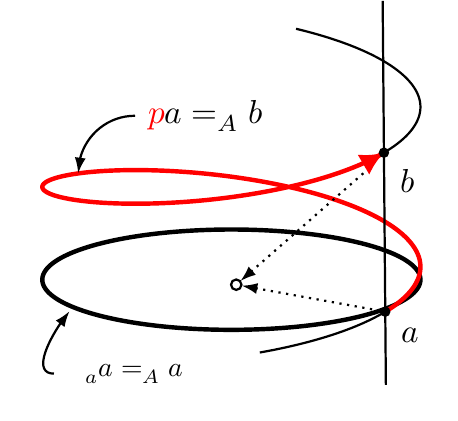
\begin{tikzpicture}[scale=2.0,
    %% background rectangle/.style={fill=olive!45},
    %% show background rectangle
  ]
  \begin{axis}[
      view={-20}{-20},
      %% axis line style = ultra thick,
      %% axis lines=middle,
      axis lines=none,
      zmax=80,
      xmax=4,
      ymax=4,
      height=8cm,
      xtick=\empty,
      ytick=\empty,
      ztick=\empty,
      clip=false,
      %% x label style={at={(axis cs:2,0.051)},anchor=north},
      %%   xlabel={$y$},
      %% y label style={at={(axis cs:0.05,2)},anchor=north},
      %%   ylabel={$x$},
      %% z label style={at={(axis cs:0.075,0,80)},anchor=north},
      %%   zlabel={$z$},
    ]
    %% \draw[<-] (-1.2,-5.7) -- node [label={west:foobar}]
    %%      {equality pencil} (0.45,-5.0);

    %% refl a
    \addplot3[domain=0:360,samples=300,samples y=1,variable=t,
      black,no marks,thick]
      %% smooth,variable=t,ultra thick]
    ({cos(t)},{sin(t)},4.5);
    \node at (-0.8,0.05) [name=refl]{};
    \node at (0,1.5)
          [name=refllabel,black,label={[scale=0.5]center:$\tj{\refl_a}{a=_A a}$}]
          {};
    %% \draw [<-] (-1.0,-5.2) -- (-0.5,-5) node
    %%       [label={[scale=0.5]east:equipoint pencil}]
    %%       {};
    %% \node at (1.1,-2.7)
    %%       [black,label={[scale=0.6,distance=-4pt]
    %%           center:{$\textcolor{red}{p}:a=_Ab$}}]
    %%       {};
    %% \node at (2.0,0)
    %%       [black,label={[scale=0.6,distance=-4pt]
    %%           center:{$\mathsf{refl_a}:a=_A a$}}]
    %%       {};
    \node at (-0.1,-0.35) [name=omphalos,black,circle,scale=0.2,draw]{};

    %%helix
    \addplot3+[domain=0.5:3*pi,samples=500,samples y=1,
      black,no marks]
    ({sin(deg(x))}, {cos(deg(x))}, {10*x/(pi)});
    %% p:a=b
    \addplot3+[domain=1.3:2.41*pi,samples=500,samples y=1,
      %% shorten >= 2pt,
      red,
      -{Latex[red,length=1.5mm,width=1.5mm]},no marks,thick]
    ({sin(deg(x))},{cos(deg(x))},{10*x/(pi)})%% NB: no semi-colon
    node [name=A,black,circle,scale=0.2,fill,pos=0,
      label={[black,scale=0.6,distance=-4pt]south east:$a$}]{}
    %% node [red,pos=0.7,label={north:$p$}]{}
    coordinate [name=pab,pos=0.5]{}
    node [name=pablabel,pos=0.4,
      xshift=6pt, yshift=10pt,
      label={[black,scale=0.6] %% ,distance=-18pt]
        center:$\tj{\textcolor{red}{p}}{a=_A b}$}]{}
    node [name=B,black,circle,scale=0.2,fill,pos=1,
      label={[black,scale=0.6,distance=-4pt]south east:$b$}]{};
      %% label={[black,label distance=0pt]east:$b$}]{};
    %% equality chord
    %%
    \draw[black,shorten >= -1cm, shorten <=-0.5cm] (A)--(B);
    \draw[-{Latex[length=1mm,width=.7mm]},black,densely dotted]
    (A)--(omphalos);
    \draw[-{Latex[length=1mm,width=.7mm]},black,densely dotted]
    ([xshift=-3pt,yshift=-3pt]B.south west)--(omphalos);
    \draw[-{Latex[length=1mm,width=.7mm]},black]
    ([xshift=-9pt]pablabel.west) to[out=180,in=90] (pab);
    \draw[-{Latex[length=1mm,width=.7mm]},black]
    ([xshift=-11pt]refllabel.west) to[out=180,in=-130] (refl);

\end{axis}
\end{tikzpicture}
\caption{Equality of two distinct values}
\label{fig:aeqb}
%% \end{subcaptiongroup}
%% \begin{subcaptiongroup}{.4\textwidth}
\end{figure}

Figure \ref{fig:aeqb} illustrates proof of equality of two distinct
values. The geometric forms are to be read as semantic symbols: not
symbols of geometric objects, but of whatever concepts we please. The
vertical line (equipoints pencil) represents identity; all points on
the line are identical. Meaning, we treat the points as coreferring
symbols. The segment joining \(a\) and \(b\) represents the type
\(a=_A b\). The red curve joining \(a\) and \(b\) (``helical loop'')
represents proof that \(a=b\). The black circle represents
\(\textsf{refl}_a:a=a\).

[To represent the coreference, draw arrows from each point in the pencil to the center of the base refl circle.

Per Frege: if a=b, then they must be coreferential, but may have
different sense. So if our helix is to represent that, we have to
treat the points a and b as coreferential, and separated in space only
to emphasize the two different ``modes of presentation'' of a and b.

Warning: the vertical equipoints pencil has no counterpart in HoTT; we
just add it for illustrative purposes, to give a graphic
representation of equality types. It makes it look like an equality
proof (helical curve) is just a deformation of an equality type
(straight line), or vice-versa, but that is not the intended meaning.
The equipoints pencil should be thought of as a kind of meta-line.

%% \subcaptionlistentry{Symmetry}
\begin{figure}[h]
\centering
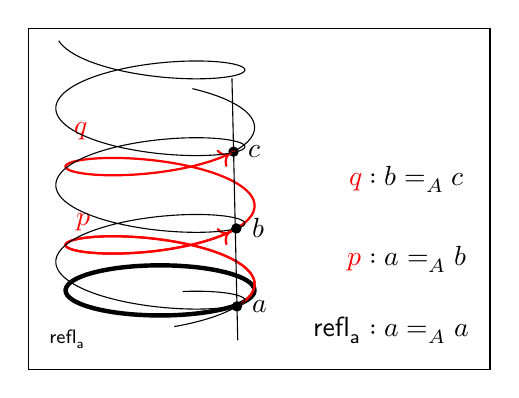
\begin{tikzpicture}[scale=1.0,show background rectangle]
  \begin{axis}[
      view={-20}{-20},
      %% axis line style = ultra thick,
      %% axis lines=middle,
      axis lines=none,
      zmax=80,
      xmax=4,
      ymax=4,
      height=8cm,
      xtick=\empty,
      ytick=\empty,
      ztick=\empty,
      clip=false,
      %% x label style={at={(axis cs:2,0.051)},anchor=north},
      %%   xlabel={$y$},
      %% y label style={at={(axis cs:0.05,2)},anchor=north},
      %%   ylabel={$x$},
      %% z label style={at={(axis cs:0.075,0,80)},anchor=north},
      %%   zlabel={$z$},
    ]
    %% \draw[<-] (-1.2,-5.7) -- node [label={west:foobar}]
    %%      {equality pencil} (0.45,-5.0);

    %% refl a
    \addplot3[samples=30,smooth,variable=t,domain=0:360,ultra thick]
    ({cos(t)},{sin(t)},4.5);
    %% \node [pos=.5,circle,fill]{};
    \node at (-0.5,1.5) [black]{$\mathsf{\scriptstyle refl_a}$};
    \node at (2.6,0) [black]{$\mathsf{refl_a}:a=_A a$};
    %% \draw [<-] (-0.98,-5.2) -- (0,-5) node [right]
    %%       {\small equipoint pencil};
    %%helix
    \addplot3+[domain=0.5:5*pi,samples=500,samples y=1,
      black,no marks]
    ({sin(deg(x))}, {cos(deg(x))}, {10*x/(pi)})
    node [name=C,black,circle,scale=0.4,fill,pos=0.875,
      label={[black,label distance=0pt]east:$c$}]{};

    %% q:b=c
    \addplot3+[domain=1.5:4.41*pi,samples=500,samples y=1,
      shorten >= 3pt,
      red,->,no marks,thick]
    ({sin(deg(x))},{cos(deg(x))},{10*x/(pi)})
    node at (0.7,-5.7) [black] {$\textcolor{red}{q}:b=_Ac$}
    node [red,pos=0.75,label={north:$q$}]{};
    %% p:a=b
    \addplot3+[domain=1.3:2.41*pi,samples=500,samples y=1,
      shorten >= 3pt,
      red,->,no marks,thick]
    ({sin(deg(x))},{cos(deg(x))},{10*x/(pi)})%% NB: no semi-colon
    node [name=A,black,circle,scale=0.4,fill,pos=0,
      label={[black,label distance=0pt]east:$a$}]{}
    node [red,pos=0.7,label={north:$p$}]{}
    node [name=B,black,circle,scale=0.4,fill,pos=1,
      label={[black,label distance=0pt]east:$b$}]{};
    %% equality pencil
    %%
    \draw[black,shorten >= -1cm, shorten <=-0.5cm] (A)--(C);
    \draw[red,fill,circle,scale=0.6] (0,1);
    \addplot3[domain=0.0:7.31*pi,samples=500,samples y=1,
      %% shorten >= 3pt,
      black,no marks,thin]
    ({1*sin(deg(x))},{0.3-1*cos(deg(x))},{9.8*x/(pi)});

\node at (1.8,-2.7) {$\textcolor{red}{p}:a=_Ab$};

\end{axis}
\end{tikzpicture}
\caption{Transitivity}
\label{fig:transitivity}
%% \end{subcaptiongroup}
%% \captionsetup{subrefformat=parens}
%% \caption{Equality proofs: \subref{fig:peqq} a huge cat,
%% and \subref{fig:aeqb} an elephant}
%% \end{adjustwidth}
\end{figure}

Figure \ref{fig:transitivity} illustrates transitivity.

%% \subcaptionlistentry{Symmetry}
\begin{figure}[h]
\centering
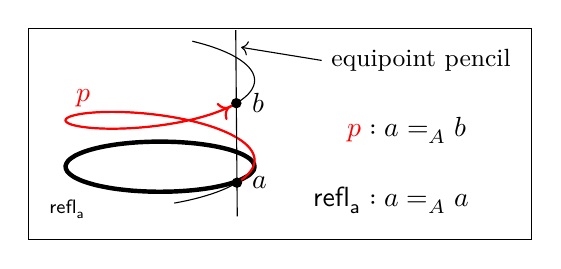
\begin{tikzpicture}[scale=1.0,show background rectangle]
  \begin{axis}[
      view={-20}{-20},
      %% axis line style = ultra thick,
      %% axis lines=middle,
      axis lines=none,
      zmax=80,
      xmax=4,
      ymax=4,
      height=8cm,
      xtick=\empty,
      ytick=\empty,
      ztick=\empty,
      clip=false,
      %% x label style={at={(axis cs:2,0.051)},anchor=north},
      %%   xlabel={$y$},
      %% y label style={at={(axis cs:0.05,2)},anchor=north},
      %%   ylabel={$x$},
      %% z label style={at={(axis cs:0.075,0,80)},anchor=north},
      %%   zlabel={$z$},
    ]
    %% \draw[<-] (-1.2,-5.7) -- node [label={west:foobar}]
    %%      {equality pencil} (0.45,-5.0);

    %% refl a
    \addplot3[samples=30,smooth,variable=t,domain=0:360,ultra thick]
    ({cos(t)},{sin(t)},4.5);
    %% \node [pos=.5,circle,fill]{};
    \node at (-0.5,1.5) [black]{$\mathsf{\scriptstyle refl_a}$};
    \node at (2.6,0) [black]{$\mathsf{refl_a}:a=_A a$};
    \draw [<-] (-0.98,-5.2) -- (0,-5) node [right]
          {\small equipoint pencil};
    %%helix
    \addplot3+[domain=0.5:3*pi,samples=500,samples y=1,
      black,no marks]
    ({sin(deg(x))}, {cos(deg(x))}, {10*x/(pi)});
    %% p:a=b
    \addplot3+[domain=1.3:2.41*pi,samples=500,samples y=1,
      shorten >= 3pt,
      red,->,no marks,thick]
    ({sin(deg(x))},{cos(deg(x))},{10*x/(pi)})%% NB: no semi-colon
    node [name=A,black,circle,scale=0.4,fill,pos=0,
      label={[black,label distance=0pt]east:$a$}]{}
    node [red,pos=0.7,label={north:$p$}]{}
    node [name=B,black,circle,scale=0.4,fill,pos=1,
      label={[black,label distance=0pt]east:$b$}]{};
    %% equality chord
    %%
    \draw[black,shorten >= -1cm, shorten <=-0.5cm] (A)--(B);

\node at (1.8,-2.7) {$\textcolor{red}{p}:a=_Ab$};

\end{axis}
\end{tikzpicture}
\caption{Second-order Equality}
\label{fig:peqq}
%% \end{subcaptiongroup}
%% \captionsetup{subrefformat=parens}
%% \caption{Equality proofs: \subref{fig:peqq} a huge cat,
%% and \subref{fig:aeqb} an elephant}
%% \end{adjustwidth}
\end{figure}

To illustrate second-level equality (figure \ref{fig:peqq}), we would
add a third point \(c\) and a helical loop \(q\) representing proof of
\(b=c\). Then we would shade the region on the surface of the cylinder
between the adjacent helical loops \(p\) and \(q\). This would look
like a ribbon wrapped helically around the cylinder. The surface would
proof of equality of \(p\) and \(q\). This figure would however lack a
graphical representation of the second-level equality type \(p =_{a=_A
  b} q\)

[To really make that work, the ribbon would meta-represent the
  equality type, and the proof would be shown by ``inflating'' the
  ribbon to make a kind of tube.

We can show the three standard properties of the equality relation. We
already show reflexivity. To show symmetry, draw another helical loop
between \(a\) and \(b\), with opposite chirality (polarity). To show
transitivity, draw loops from a to b, and from b to c, and then from a
to c.



\section{Notes}

\subsection{Infinities}

\href{https://en.wikipedia.org/wiki/Axiom_of_infinity}{Axiom of Infinity}

\href{https://en.wikipedia.org/wiki/Finitism}{Finitism}

\subsection{Non-well-founded sets}

\citetitle{nonwf_deduction} \cite{nonwf_deduction}

\subsection{Recursion and Corecursion}

If you check for a base case, it's recursion; otherwise it's
corecursion.

Equivalently, if the domain type is defined by induction, it's recursion. Otherwise, it's corecursion.

\href{http://blog.ezyang.com/2013/04/the-difference-between-recursion-induction/}{The Difference between Recursion \& Induction}

Or: define types by induction, functions by recursion?

Some writers say the opposite: recursion defines, induction proves.

Better: induction defines types, recursion defines functions on types.

Or: induction is semantic, recursion is syntactic. In which case we would express induction by writing recursion.

Does recursive merely mean self-referential? Note there is no
self-reference in the standard definition of \(\Nat\) by induction.
Except maybe insofar as the ctor definitions refer to the type name.

Etymology: recursion = running \textit{back}, i.e. back to the
beginning, returning to the base case. ``Recursion'' cannot mean
``self-referential'', so maybe it was coined specifically to the
``iterating back to base'' process. Then induction would only refer to
building up new from old, without self-reference.

Makes sense. Function definitions analyze their arguments and then
possibly recur on part of the arg.

\subsection{Programming}

\citetitle{goguen1996algebraic} \cite{goguen1996algebraic}

\subsection{Assumptions}

Compare: reasoning with counterfactuals v. reasoning from assumptions

Counterfactuals make no assumptions.

\subsection{Dark Logic}

Compare coinductive and probabilistic thinking. Both involve reasoning
with imperfect information.

Coinduction assumes the definiendum is already determined. Like dark
matter.

We can express coinduction as inference rules in a logic. And
reasoning by coinduction seems qualitatively different than inductive
reasoning.

Does a co-logic make sense?

We have cofunction, a function defined co-inductively. By
Curry-Howard, that gives us co-implication. What about co-conjuction,
co-disjunction etc.?

Conjunction. Elimination rule assumes that we can be given a token
\(p\) where \(\tj{p}{A\lkand B}\), such that the meaning of \(p\) is
determinate, but it does not assume that \(p\) has the form of a pair.

We can \textit{define} as many distinct function implementations as we
like for a given function type, say \(\Nat\func\Nat\). What about
conjuction and disjunction?

Linear logic shows that we need at least two distinct
``implementations'' for both. Or does it. It has different inference
rules, so its not a matter of different implementations of the same
type.

But then under what circumstances would it make sense to have more
than one implementation of \(\lkand\)? Or: when would it make sense to
say \(A \lkand B\) is not unique? More precisely that it has only one
ctor?

We can have many function implementations because of the way we
interpret \(\func\). It must be a procedure capable of producing a B,
given an A, an A-to-B machine. That makes it a meta-machine. But all
inference rules are meta in this way. But \(\func\) starts with a
token-producing machine, not a meta-matchine. Can we think of
conjunction like this? Start with a pair of machines capable of
producing A and B tokens out of ylem; the \(\lkand\) machine turns
those machines into \(A\lkand B\) tokens. Then we can have different
implementations of those machines. One that produces tokens out of
unicorn blood, for example.

So the type of all A-to-B machines is \(A\func B\). To produce one we
must build it ourselves, using the lambda calculus as a tool.

Leprechaun lambdas.

But we do not have a lambda calculus, or any calculus, that will allow
us to build an implemention of a cofunction cotype. Such machines can
only be built by leprechauns, according to leprechaun engineering
standards, and they are permanently sealed, so it is impossible for us
to open one up and inspect the construction.

So if we need to do something useful with a machine of such a type, we
just assume that we can pick out an arbitrary unit from the limitless
stock of prebuilt machines.

No, better is, we go down to the leprechauns and tell them what we
want: we give them the equations specifying how the head and tail
should work, and they build us one from spec. That's how we can think
of the codefining equations for a cotype as specifications rather than
axioms. Giving us three ways to think of them: as axiomatic truths, as
rules of interence, and as engineering specifications.

Leading to the idea that induction is semantic, and coinduction is
syntactic.

We only need the lambda leprechaums if we insist on metaphysics.
Classically, for computable functions, we have the idea that they
exist, and Turing Machines or some other model allows us to express
them formally. So there remains an ontological gap between a function
and its representation as, say, a lambda definition. Since our models
of computation work so well, and since they are constructive, we have
little compunction thinking that the functions expressed by lambda
definitions exist, either eternally, or in virtue of our construction.

Things are different for cofunctions, however. We don't have a good
reason for thinking they exist. We cannot construct them after all; we
cannot even imagine what it would take to construct them, since the
very concept of construction seems to mean finitude.

Actually the logic is similar to the way we think about the infinities
associated with our constructions. We're inclined to think the natural
numbers exist \textit{in toto}, because we know that we can construct
any particular natural number. So we make a kind of metaphysical leap
from the existence of each natural number to the existence of their
infinitude. Of course, intuitionism rejects the possibility of a
``completed infinity''. Usually we just abuse the language, and say
``\(\Nat\) exists'' when what we really mean is that each number
exists or can be constructed. In any case, the critical point is that
we need not presuppose the existence of the totality \(\Nat\) in order
to think that \textit{each} natural number exists.

We can \textit{almost} think about colists in the same way. Each
colist is isomorphic to \(\Nat\), and we can extract each prefix as a
finite list, just as we can construct each natural number. But
extraction of a prefix depends on use of the co-constructors and the
assumption that the colist antecedently exists - if it did not, then
the co-constructors would have nothing to work with, and we would not
be able to extract a finite list. So it looks like the logic of
coinduction inescapably presupposes some metaphysical commitments.

How can we get around this, and ``explain'' such codata without
metaphysics? I think the intuitionist approach is to think in terms of
approximations. We do not need ontological commitments to understand
codefinitions etc. as specifications. In other words, if we think
syntactically instead of semantically. Then we can approximate a
colist by constructing successive prefixes, without any metaphysical
presuppositions about the existence or otherwise of the whole colist.

But note: we're not quite thinking entirely syntactically. We're just
treating syntax as primary. We then endow the syntax with meaning.
I.e. its not empty syntax, its more like syntax with contingent or
implied semantics. We work with the syntax on the understanding that
it has a kind of approximative semantics.

Counter-factual semantics: if colists were to exist, then we would be
able to extract finite prefixes. But the converse does not hold: if we
can extract prefixes, then colists exist. So our ability to extract
prefixes is rendered intelligible by the counter-factual, but we
cannot then conclude that colists exist. We can say that the syntax
has counter-factual semantics. Meaning that the counter-factual makes
the things we say about colists meaningful, but does not entail
metaphysical commitments.

This would require that we reject the usual reading of ``semantic'' as a
synonym of ``denotational'' or ``representational''.

Sadly, the logic and semantics of counterfactuals is very complex. But
they're easy enough to understand informally and that's enough for
present purposes.

\citetitle{sep-counterfactuals} \cite{sep-counterfactuals}



\subsection{Coinduction Rules}

Double entendre: rules of coinduction v. dominance of coinduction

The logic of coinduction is the logic of empirical science.

Difference between scientific induction and mathematical induction:
the latter involves an element of necessity that is completely lacking
in the former. Modality of necessity v. possibility. The inferences
delivered by scientific induction are always contingent. They may be
undermined in two ways. Additional experimental evidence may render
them invalid, and changes to theory may render them inappropriate, for
lack of a better term. Einstein gave us a vivid example of the latter
when he redefined the concept of gravity, and thereby forced a
reconceptualization of the entire body of inferences underwriting
theoretical physics.

But if scientific and mathematical induction differ in this
fundamental way, why do we call them both ``induction''. One reason is
historical: the concept of induction is much older and more familiar
than the concept of coinduction, which only began to emerge as a
distinctive concept relatively recently.

Once we have a clear understanding of coinduction, it becomes clear
that what we all scientific induction is actually coinduction.

Latent variables and measurement. What's the difference between a
``latent variable'' in the social sciences, like the Big 5 personality
traits (extraversion, agreeableness, openness, consientiousness, and
neuroticism), and a concept like ``mass'' in physics? After all, mass
is just as ``latent'' as neuroticism. We cannot directly observe mass;
the best we can do is observe measurements whose results, we theorize,
are ``caused'' by mass. Those measurements are so precise and reliable
(replicable), and the predictions we make based on those experimental
results are so good, that we have seen fit to elevate the concept of
mass to a kind of axiomatic status. That's an example of co-inductive
reasoning: we use observations to draw inferences about the machinery
behind the appearances.

From this perspective, the only difference between such (mostly)
undisputed concepts like mass and very debatable concepts like the
latent variables of psychology is measurement. The problem with
``neuroticism'' is that we have no good way to measure it. That could
be because we do not have a good theory that would enable us to
explain how neuroticism affects observable properties or behaviors, or
it could be because we lack the instruments of measurement we need to
make good observations. But if we did have a good way of measuring
neuroticism, and such measurements allowed us to make reliable
predictions about future measurements, then we would be justified in
bestowing on the concept of neuroticism the same status we grant to
the concept of mass. And the kind of reasoning involved would be
coinduction.

Pavlov's dog.

\subsection{Imaginary Numbers}

The imaginary number is \(i\), the square root of negative one. The
acceptance of \(i\) as a genuine number marked a radical shift in our
concept of number, a movement away from number as magnitude and
quantity to a more abstract notion in which measurement plays no
essential role. It threw a spanner in the metaphysical works of
traditional mathematics. Trying to imagine \(\sqrt{-1}\) is like
trying to imaging a round square.

But it was not the first imaginary number, if by ``imaginary'' we mean
something metaphysically puzzling, something whose existence we have a
hard time imagining.

But \(i\) is only the most famous imaginary number. Zero and negative
numbers are just as metaphysically puzzling.

[What's the point? Aside from historical interest, demonstrate how a
  pragmatic order of explanation can account for such things. Does
  this have any implications for how we do type theory? Other than
  clarify and refine meanings?  Also: make the relation between logic and mathematics more clear.]

\subsubsection{Zero}

The Greeks lacked zero for a reason. Their mathematics was
demonstrative and constructive: the way to prove something was to
demonstrate its construction. But you cannot demonstrate nothing.
Hence, no zero concept.

If zero \textit{exists}, then it cannot be nothing.

Consider the usual inductive methods of constructing the natural
numbers. The most primitive way to do it is to concatenate a tally
mark. The successor operation is something we do -- add another tally
mark -- which we need not make explicit. So we have \(1\eqdef\Stroke{1},
2\eqdef\Stroke{2}, 3\eqdef\Stroke{3}\) etc.

This is fine if we do not need zero. We can define addition, for
example. Notice in particular that there is no distinguished base
case; every \(\Stroke{1}\) is alike, and to construct a number, you
start from nothing, not zero.

Most presentations, though, follow Peano's example and define a base
case and use a distinguished symbol for it (\ZNat, \(\mathbb{0}\),
etc.). This requires two axioms, one affirmative and one negative:
\ZNat{} is a natural number, and \ZNat{} is not the successor of any
natural number.

We start with \ZNat{} and \SNat{}, and we can build \ZS, \ZSS, etc.
\textit{ad libitum}.

But what do \ZNat{} and \SNat{} denote? We have two options for \ZNat:
either it denotes something, or it does not.

If \ZNat{} exists, then we're forced to concede that the number \(1\)
is actually a two, since it is the combination of two things:
\(1\eqdef \ZS\). Under this operation, \SNat{} is also a thing:
the successor \textit{operation} is not \SNat; rather it is what we do
when we add \SNat{} to a natural number. But then \SNat{} would be a
special kind of thing, something that cannot stand alone, since
otherwise \SNat{} itself would be a number (maybe we need another
axiom stating ``\SNat{} is not a natural number''.)

Or, we could treat \SNat{} as a kind of primitive, undefined,
function-like thing that takes any natural number to its successor.
Then we would have two ways to interpret it. The non-constructive way
would presuppose that the successor of each \(n\) already exists, and
the job of \SNat{} is to point to it, so to speak. The constructive
interpretation would treat \SNat{} as some kind of mechanism that, given
an existing natural number (as a kind of raw material), produces a new
one.

Under a constructive interpretation, \ZNat{} could not merely denote
something that already exists; but for \ZS{} to be intelligible
under this interpretation, \ZNat{} would have to denote
\textit{something}, so that \SNat{} would have the raw materials it
needs to produce a new number. So we would be compelled to think of
\ZNat{} as a kind of productive machine just like \SNat, except that
\ZNat{} would need no raw materials to get started. It would create
something from nothing.

So the construction of \(\Nat\) is already metaphysically puzzling.

So far we have a distinguished first natural number \ZNat, but it does
not yet behave like zero. In fact, under the rules we have so far, it
behaves like \(1\). To make it behave like we expect zero to behave ,
we need to add some constraints on addition: \(n + \ZNat = n,\ \ZNat +
n = n\). And again there are two ways to interpret this. One is to
think that the introduction of these axioms changes the meaning of
\ZNat. They confer a special property not on the \ZNat machine itself,
but on its output: when that ``\ZNat-thing'' used in an addition it
adds nothing. The other strategy is to think that the introduction of
the axioms changes the meaning of addition: it now examines its
operands, and discards any equal to \ZNat.

No matter how you cut it hermeneutically, zero is metaphysically
puzzing.

[What's the point? To motivate a pragmatic order of explanation.]

\subsubsection{Negative Numbers}

It's equally easy to see why the Greeks had no truck numbers. Negative
quantities and magnitudes are unimaginable. ``Line of length \(-2\)''
is absurd.\footnote{I distinctly remember first encountering negative
numbers in my first Algebra class in junior high school, and being
puzzled as to how a number could possibly be negative. Subtraction is
one thing; a negative number is a whole `nother thing.}

Historically, the negative numbers emerged in tandem with zero. The
Arabic-speaking mathematicians who invented algebra did so for
practical reasons: algebra is a tool that makes it easier to balance
the books. Negative quantities may be inconceivable, but
\textit{deficits} are easily understandable, nor do they presuppose
any metaphysical commitments. Zero is what you get with balanced
books: no difference between debits and credits. Negative numbers? You
owe somebody. Positive? Sombody owes you.

The algebraic perspective is compatible with number-as-quantity. A
negative number represents a quantitative deficit. It's still ``...of
something''; not just \(-3\), but \(-3\ \textit{dirhams}\) (or goats
or acres or whatever), that is, a deficit of \(3\) \textit{of
  dirhams}, the quantity you need to balance your books. If they had had
formal logic, they would have invented Linear Logic.

\subsection{Games}

The games we're talking about are not the games of game theory. Those
games have winners and losers. Our games are deontic: they involve a
set of rules that players are obligated to follow if they want to
count as playing the game at all. You cannot lose that kind of game;
if you do not follow the rules, then you are not playing the game.

You can push chess pieces around, but if you do not obey the rules of
chess, then you are not playing chess. An invalid inference is not an
inference; a program that fails to compile is not a program. A proof
that does not obey the rules of inference is not a proof.

\subsection{Logical Pluralism}

Is logic one or many? These days there are many logics to choose from.
The question is whether they are all species of a single genus.

To really understand a logic, you must master the use of a calculus. A
calculus for a logic defines the language you use to express reasoning
within the logic. But there are many calculi to choose from, each of
which can be used for different logics. The calculi themselves have
various properties, so they offer different perspectives on reasoning.
So the really \textit{really} understand a logic, you should master
multiple calculi.

We can also ask whether all logical calculi are species of a single
genus. This suggests that the calculi themselves are worthy objects of
study, and the answer is clearly yes. The study of such calculi
usually falls under the rubric ``Proof theory'', but be forewarned
that, as its name suggests, Proof Theory also studies other things,
such the nature of proofs.

We can ask again: are all proofs species of a single genus?

Is there more than one consequence relation? And is consequence the
same as inference?

Finally, we can ask whether all inferences are species of a single
genus. This, like our other questions about logical plurality, is a
philosophical question, whose answer is by no means obvious. For
example, take Classical and Intuitionistic logics. One of the main
differences between them is that the latter includes the Law of
Excluded Middle (LEM)\footnote{Sometimes called the Principle of
Excluded Middle (PEM)}. This law says that every proposition is either
true or false; there is no middle option. So if we do not know whether
a particular proposition \(P\) is true or false, at least we know that
it \textit{must} be one or the other. This means that if we assume it
is false and then prove a contradiction, we not only can but must
\textit{infer} that it is true. Under Intuitionistic logic, things are
different. We can infer that it is not true, but we must not infer
that it is false. Does this difference reflect a \textit{difference in
  kind} of the inferences involved in the two logics?

Variety of form does not entail plurality of content. FOL can be
expressed in many calculi whose forms vary greatly, but they all
express FOL.

See \citetitle{sep-logical-pluralism} \parencite{sep-logical-pluralism}
for more information.


\subsection{Centrality of Inference}

The one thing all logical calculi have in common is a notion
inference. It should be obvious that any calculus we want to use to
express reasoning must have a means of expressing inference, since
inference is the central concept of reasoning. But it's less obvious
that this should be the \textit{only} thing they must have in common.

What about proof? No, that's an add-on; you can have a logical
calculus that does not define what counts as a proof. Most do define
proof formally, but it is not required. Remember that logic is about
consequence, not proof. The concept of proof is parasitic on the
concept of consequence.


\subsection{Residuation}

Deduction theorem: inter-convertability between consequence and
implication.

Implication requires modus ponens to detach the conclusion.
Consequence does not. So this is a kind of asymmetry between the two.


Bimbó says that operators are residuals of operators, for example
p. 120 says \(\lollipop\) is the residual of \(\circ\) in linear
logic.

But Restall makes it look like residuation is about operands, not
operators.

Must be that \(\linfer\) is the residual of \(→\), or vice versa?


\textquote[\citetitle{sep-logic-substructural} \cite{sep-logic-substructural}]{
Logic is about logical consequence. As a result, the conditional is a central notion in logic because of its intimate connection with logical consequence. This connection is neatly expressed in the residuation condition (also known as the deduction theorem):

\[p,q\linfer r\ \text{if and only if}\ p\linfer q\rightarrow r\]

It says that \(r\) follows from \(p\) together with \(q\) just when \(q→r\)
follows from p alone. The validity of the transition from \(q\) to \(r\)
(given \(p\)) is recorded by the conditional \(q→r\).

This connection between the conditional and consequence is called
residuation by analogy with the case in mathematics. Consider the
connection between addition and substraction. \(a+b=c\) if and only if
\(a=c−b\). The resulting \(a\) (which is \(c−b\)) is the residual,
what is left of \(c\) when \(b\) is taken away. Another name for this
connection is the deduction theorem.}

The term makes perfect sense for arithmetic. It is a standard term in
statistics, where the residual is the difference between an predicted
and observed values. But its harder to see how to give it an intuitive
reading in logic. It seems to be motivated by formal analogy:

\begin{align}
  a+b &= c & \text{arithmetic sum equals c} \\
  a &= c - b & \text{arithmetic residual equals difference} \\
  b &= c - a \\
  p,q &\linfer c & \text{sum entails c} \\
  p &\linfer q→r & \text{residual p entails implication} \\
  q &\linfer p→r
\end{align}

The formal analogy is clear, but it's hard to see how arithmetic
difference and implication are related. But I think the formal analogy
does reflect substantial analogy.

The arithmetic residual is what you get when you ``undo'' a sum. Just
focus on the LHS: the residual is what you get when you remove a
summand. But what makes it a ``residual'', instead of just a summand?
The relation of addition and subtraction on the one hand, and equality
on the other. Residuation expresses that link.

Or: residuation preserves equality. If you remove one of the summands,
what do you need to do to restore equality? Make that move and the remaining summand is a residual.

So in logic: residuation preserves entailment. If you remove one of
the conjuncts from the antecedent, what do you need to do to preserve
the entailment?  You convert the conclusion to an implication. So conjunction is the residual of implication.

Better: residuation as an algebraic (-like) operation whose purpose is
to restore inferential equilibrium. If you break the whole, by
removing a part on the left, then to mend (al-jabr) and restore the
balance (al-muqabala) you must treat the RHS. In the case of ``and''
on the LHS, the remedy is to introduce a new operator, \(→\), on the
RHS.

Restall seems to get this wrong, calling residuation a relation
between the conditional and consequence. I think it is a relation
between two operators mediated by consequence. After all the
conditional is not the only operator that can be entailed; in fact
they are all essentially related to entailent. The general form: if
you remove an operand on the LHS, what do you need to do on the RHS in
order to preserve the entailment? The answer will involve another
operation.

For logic, the residual \(p\) is what you get when you remove the
summand (or ``factor''?) \(q\) from the sum \(\ulcorner
p,q\urcorner\). What makes it a residual instead of a mere premise?
The relation between summing (\(\ulcorner ,\urcorner\)) and
implication.

In a real sense is it is a lack. Remove one of the conditions of
production and the output lacks something.

Treat \(p,q\linfer r\) as a binary function. If you want to convert it
to a unary function, you remove one of the parameters, and you output
another unary function that takes the removed parameter as its arg.

In other words, this kind of residuation is just currying. Which makes
the deduction theorem a kind of currying. The residual is the
second-level (``wrapped'') unary function.

How nice, this gives us a piece of terminology we can use to talk
about currying. For each parameter of any binary function, we have a
residual, which is the unary function that takes the other parameter
as an argument. E.g. if we have \(f(a,b)→c\), then the residual of
\(a\) is the unary function that takes \(b\) as an argument (and may
also use a, but not as an arg) and returns \(c\).

For arithmetic, residuals are numbers. For logic, they are operators.
Implication is the residual of conjunction, because it is what you
need to restore entailment after you remove conjunction. Its ``what's
left over'' after removal of conjunction.

This is incredibly obvious once you see it. Why did it take me so long
to see it?

Are residuals always implication operators? Seems they must be; to
restore entailment, you must add implication.

\begin{itemize}
\item \(a + b = c\) the arithmetic sum of a and b equals c.
\item \(a = c - b\) the residual a is what's left when you subtract b from c
\item \(p,q\linfer r\) the logical sum of p and q entails r
\item \(p\linfer q→r\): p is what is left when you ...?
\end{itemize}

Here ``logical sum'' does not mean ``logical conjunction''
(\(\land\)). It is meant to convey the ``structural'' concept of ``p and
q together'' \textit{outside} of the logic.

The algebraic operation that yields the residual is the same on both
sides of the equation symbol. But the logical operation is not; it's
not even symmetrical.  To get the residual, we need to:

\begin{itemize}
\item remove \(q\) from the sum on the LHS
\item combine it (``add'' it?) on the RHS in a particular way
\end{itemize}

\subsection{Arbitary Choice Operator}

These calculi depend heavily on assumptions. The premises of inference rules are assumptions. For type systems, they look like \(a:A\), i.e. assume a is of type A.  More explicitly, assume A is non-empty and a is an \textit{arbitrary} token of type A.

Currently square brackets are used to make assumptions explicit, but
they are also used for other purposes.

We can make this more explicity by defining a choice operator. For
example, we can borrow Hilbert's epsilon. Then \(\epsilon \phi\) would
mean ``choose arbitrary proposition \(\phi\)'', and \(\epsilon a:A\)
would mean ``choose arbitrary a of type A''. Same as the assumption
above, but explicit.

Examples:

\begin{center}
\AxiomC{$\Gamma$}
\AxiomC{$[\phi]$}
\noLine
\UnaryInfC{$\vdots$}
\noLine
\UnaryInfC{$\psi$}
\BinaryInfC{$\phi\rightarrow\psi$}
\DisplayProof
\hskip1em
\rightarrow
\AxiomC{$\Gamma$}
\AxiomC{$\epsilon\phi$}
\noLine
\UnaryInfC{$\vdots$}
\noLine
\UnaryInfC{$\psi$}
\BinaryInfC{$\phi\rightarrow\psi$}
\DisplayProof
\end{center}

With types:

\begin{center}
\AxiomC{$\Gamma$}
\AxiomC{$[\phi:A]$}
\noLine
\UnaryInfC{$\vdots$}
\noLine
\UnaryInfC{$\psi:B$}
\BinaryInfC{$\phi\rightarrow\psi:$}
\DisplayProof
\hskip1em
\rightarrow
\AxiomC{$\Gamma$}
\AxiomC{$\epsilon\phi$}
\noLine
\UnaryInfC{$\vdots$}
\noLine
\UnaryInfC{$\psi$}
\BinaryInfC{$\phi\rightarrow\psi$}
\DisplayProof
\end{center}

\subsection{Strategies}

A common technique is to define use of a connector indirectly.  Instead of showing what follows directly, use an intermediary.

\subsection{Disjunction}

We actually need a choice operator to make sense of disjunction, or
more precisely, to make our calculus work for disjunction.

To see why, start with conjunction: \(A, B\linfer A\lkand B\). The
usual way to gloss this is something like ``If A is true and B is
true, then A\(\lkand\) B is true''. But we need to be more explicit.
Implicit in the standard gloss is that A and B are
propositions.\footnote{TODO: note on Martin-Löf}. Also implicit is
universal quantification; what we really mean is ``For all
propositions A and B, if A is true and B is true, then A\(\lkand\) B
is true''.

Note that in \(A, B\linfer A\lkand B\) the only symbol in the
conclusion that is not in the premises is \(\lkand\).

To make the interpretation of such formulae fully explicit, we have
two options. We can use the universal quantifier, and write something
like \(\forall A, B: A, B\seqso A\lkand B\). Or we can use our choice
operator, and write \(\choice A, \choice B\seqso A\lkand
B\).\footnote{Read ``if arbitrary A is true and arbitrary B is true
then A\lkand B is true''.} But this leaves the domain of
quantification implicit; the be really explicit, we would have to find
a way to indicate that A and B range over propositions (for
\(\forall\)), and that \(\choice A\) means ``for arbitrary proposition
A''.

Now look at the standard introduction rules for disjunction. We have
two, one for the left disjunct and one for the right: \(A\seqso A\lkor
B\) and \(B\seqso A\lkor B\). The problem is immediately evident:
\(B\) appears in the conclusion but not in the premises. The rules
introduce more than just \(\lkor\); they also introduce \(B\). But
\(B\) is a non-logical symbol, so this makes no sense.

The implicit logic is simple enough. We take \(A\seqso A\lkor B\) to
mean ``If A is true, then A\lkor B is true whether B is true or not'';
more precisely, ``For all propopsitions A, if A is true, then for all
propositions B, \(A\lkor B\) is true''. In other words, to make sense
of the introduction rules for disjunction, we're forced to commit to
\textit{two} implicit universal quantifications. Symbolically, using
\(\ulcorner :\mathbb{P}\urcorner\) to mean ``ranging over
propositions'':

\[\forall A:\mathbb{P}, A\seqso\forall B:\mathbb{P}, A\lkor B\]

But this is cumbersome.  Using \(\choice\) we get a more concise expression

\[\choice A\seqso A\lkor \choice B\]

But now we're back where we started: the conclusion contains symbols
that are not in the premises. What we need is a way to mention \(B\)
in the premises. If we try \(\choice B\), then we get the same
premises as the introduction rule for \(\lkand\). That's because we
read the meta-symbol \(\ulcorner ,\urcorner\) as ``and'', so when use
as premise(s) \(\ulcorner\choice A,\choice B\urcorner\) must be
glossed ``if arbitrary A is true and arbitrary B is true'', and this
gives us the wrong scope of quantification for disjunction. We need to
quantify B \textit{after} A, or choose arbitrary \(B\) \textit{after}
we've chosen arbitrary \(A\). But that means that \(B\)
\textit{cannot} be involved in the premise, which in turn suggests
that it must be the introduction rule itself that injects, not just
symbol \(B\), but also its quantification.

In other words, ``natural'' \(\lkor\), the kind defined by
introduction and elimination rules, presupposes a subordinate
quantification. It follows that the introduction rules do more than
just introduce the logical constant. But that's ok. Nothing says that
such rules must introduce the constant \textit{and nothing else}. The
only constraint is that the additional ``stuff'' introduced must not
have any ``side effects'', that is must not turn any other good
inferences into bad ones or vice-versa. Which is to say, each
introduction rule must be a \textit{conservative extension} of the
language.

Who cares? Why bother, except to make the logic fully explicit? Well,
a finer degree of explicitation is not nothing. In this case, it will
help us better understand typed calculi.

\subsection{Vernacular}

The vernacular is the language of prelogic.

The vernacular is not meta-logic. It uses logic, but is not
\textit{about} logic.

\subsection{Proof Theory}

\textquote[\citetitle{DBLP:journals/sLogica/Prawitz19} \cite{DBLP:journals/sLogica/Prawitz19}]{I see the question
  what it is that makes an inference valid and thereby gives a proof
  its epistemic power as the most fundamental problem of general proof
  theory.
  \vskip-2em
  \[\vdots\]
  \vskip-1em
  ``In my plea for general proof theory, I suggested a number of obvious topics: the question of defining the concept of proof, investigations of the structure of proofs, the representation of proofs by formal derivations, and the finding of identity criteria of proofs that answered the question when two derivations represent the same proof.
  \vskip-2em
  \[\vdots\]
  \vskip-1em
  ``But I still think that the problem of defining the concept of proof or the validity of inference is the most fundamental problem of general proof theory...
}

Remember that the concept of proof presupposes a concept of
consequence (or inference), so a theory of proof lives or dies by its
notion of consequence.

Proof is usually defined as (roughly) a tree or chain or anyway
structure of ``connected'' inferences, expressed as derivation
structure in the calculus.

\subsection{Proof Identity}

We can have different proofs for the same proposition. How can we tell
if they are equal? This is an unsolved problem. But it accounts for
the complexity of equality in HoTT.

Compare: deciding when two functions are equal, that is, when two
implementations of the same function are equal. We know the criteria
for deciding: same outputs for same inputs. But its possible that two
different algorithms could accomplish that. Would they count as the
identical? Extensionally, yes; intensionally, no. Do they need to be
the same program?

\subsection{Proof-irrelevance}
Propositions are forgetful. They do not remember how they came to be.
E.g. \(A\land B\) does not know that it was formed using the intro
rule. In fact there is no reason to assume that it was. This is easier
to see in a type system, where we would have \(p:A\times B\), meaning
that \(p\) is a token (term, instance, etc.) of type \(A\times B\), or
equivalently \(p\) is a proof of the type. This tells us nothing about
how \(p\) came to be.

\subsection{Closed-World Assumption}



\subsection{Codefinition}

Introduction (right) rules define; elimination (left) rules co-define.
Elimination rules make an assumption, that the proposition they are
using is ``defined''. But that is just an assumption. The elimination
rule itself says what can be done with the propositon, but this cannot
count as a definition \textit{of} the proposition. Definitions, under
this perspective, tell us how things are put together. They do not
tell us how to \textit{use} what we have put together; in particular
they to not tell us how to disassemble composites.

Codefinitions do that. They tell us what we can do with the composite,
\textit{on the assumption} that it is already ``defined'' in some
indeterminate way. But they do \textit{not} assume that is was
constructed by an introduction rule.

Take \(\land\) for example. Here is the way the rules are often
presented, with the context and \(\linfer\) omitted for simplicity's
sake:

%% Logical And
%% \begin{center}
%% \AxiomC{$A$}
%% \AxiomC{$B$}
%% \BinaryInfC{$A\land B$}
%% \DisplayProof
%% \hskip 1.4em
%% \AxiomC{$A\land B$}
%% \UnaryInfC{$A$}
%% \DisplayProof
%% \hskip 1.4em
%% \AxiomC{$A\land B$}
%% \UnaryInfC{$B$}
%% \DisplayProof
%% \end{center}

The rule on the left defines \(A\land B\): you build a conjunct
\(A\land B\) from an A and a a B. The two on the right jointly
co-define it: given (that is, \textit{assuming}) \(A\land B\), you
can extract A or B or both.

This example is a bit misleading, though, since the syntax \(A\land
B\) suggests that the elimination rules operate by extracting A or B
syntactically. That is not the case. We can make this more evident by
rewriting the rules as follows to make the assumptions explicit:

%% \begin{center}
%%   \AxiomC{$P$}
%%   \LeftLabel{$\scriptstyle\text{[P a \(\land\) conjunct]}$}
%%   \UnaryInfC{$first(P)$}
%%   \DisplayProof
%%   \hskip 1.4em
%%   \AxiomC{$P$}
%%   \LeftLabel{$\scriptstyle\text{[P a conjunction]}$}
%%   \UnaryInfC{$second(P)$}
%%   \DisplayProof
%% \end{center}

In type theories, conjunction corresponds to product types:

%% \begin{center}
%%   \AxiomC{$p:A\times B$}
%%   \UnaryInfC{$first(p):A$}
%%   \DisplayProof
%%   \hskip 1.4em
%%   \AxiomC{$p:A\times B$}
%%   \UnaryInfC{$second(p):B$}
%%   \DisplayProof
%% \end{center}

In other words, the elimination rules tell us that we can extract a ``first'' element and a ``second'' element from any conjunct.

To make this work we also need to \textit{harmonize} the definition
and co-definition. In this case that means ensuring that we can
control which element we extract. The definitional introduction rule
says we can combine A and B; the codefinitional rules must allow us to
reliably retrieve either one. In other words, we need to ensure that
if we construct \(A\land B\), then \(first\) will extract A.

In the case of our first example, this is already evident from the
syntax of the rules. But if we want to use the second style, we cannot
depend on the meanings of \(first\) and \(second\) to guarantee this;
after all, we could have used some other terms, such as \textit{left}
and \textit{right}, \textit{red} and \textit{blue}, or even
\textit{foo} and \textit{bar}. Whatever terms we use, we need to
establish a corresponds between the eliminator terms and the
constructor. The only way to do this is by setting down a meta-axiom
that says that the first argument to the constructor corresponds to
one extractor, and the second to the other. Something like this
\(red(A\land B)\eqdef A\), \(blue(A\land B)\eqdef B\)

Note: the extractors (\textit{first}, \textit{second}, or whatever)
use function application syntax, but they are not functions. They are
codefiners \textit{by} definition, but do not themselves \textit{have}
definitions.

Usually this harmonization is taken for granted, because its obvious
and tedious to write out.



\chapter{Bibliography}

%% \addcontentsline{toc}{section}{References}
\printbibliography[heading=none]


%% \printnoidxglossaries % iterate over all indexed entries
\addtocontents{toc}{subsection}
\addcontentsline{toc}{section}{Glossary}
\printglossaries
%% \makeatletter
%% \addtocontents{toc}{\let\protect\l@section\protect\l@subsection}
%% \label{glossary}
%% \makeatother


\end{document}
